\documentclass[twoside]{book}

% Packages required by doxygen
\usepackage{fixltx2e}
\usepackage{calc}
\usepackage{doxygen}
\usepackage[export]{adjustbox} % also loads graphicx
\usepackage{graphicx}
\usepackage[utf8]{inputenc}
\usepackage{makeidx}
\usepackage{multicol}
\usepackage{multirow}
\PassOptionsToPackage{warn}{textcomp}
\usepackage{textcomp}
\usepackage[nointegrals]{wasysym}
\usepackage[table]{xcolor}

% Font selection
\usepackage[T1]{fontenc}
\usepackage[scaled=.90]{helvet}
\usepackage{courier}
\usepackage{amssymb}
\usepackage{sectsty}
\renewcommand{\familydefault}{\sfdefault}
\allsectionsfont{%
  \fontseries{bc}\selectfont%
  \color{darkgray}%
}
\renewcommand{\DoxyLabelFont}{%
  \fontseries{bc}\selectfont%
  \color{darkgray}%
}
\newcommand{\+}{\discretionary{\mbox{\scriptsize$\hookleftarrow$}}{}{}}

% Page & text layout
\usepackage{geometry}
\geometry{%
  a4paper,%
  top=2.5cm,%
  bottom=2.5cm,%
  left=2.5cm,%
  right=2.5cm%
}
\tolerance=750
\hfuzz=15pt
\hbadness=750
\setlength{\emergencystretch}{15pt}
\setlength{\parindent}{0cm}
\setlength{\parskip}{3ex plus 2ex minus 2ex}
\makeatletter
\renewcommand{\paragraph}{%
  \@startsection{paragraph}{4}{0ex}{-1.0ex}{1.0ex}{%
    \normalfont\normalsize\bfseries\SS@parafont%
  }%
}
\renewcommand{\subparagraph}{%
  \@startsection{subparagraph}{5}{0ex}{-1.0ex}{1.0ex}{%
    \normalfont\normalsize\bfseries\SS@subparafont%
  }%
}
\makeatother

% Headers & footers
\usepackage{fancyhdr}
\pagestyle{fancyplain}
\fancyhead[LE]{\fancyplain{}{\bfseries\thepage}}
\fancyhead[CE]{\fancyplain{}{}}
\fancyhead[RE]{\fancyplain{}{\bfseries\leftmark}}
\fancyhead[LO]{\fancyplain{}{\bfseries\rightmark}}
\fancyhead[CO]{\fancyplain{}{}}
\fancyhead[RO]{\fancyplain{}{\bfseries\thepage}}
\fancyfoot[LE]{\fancyplain{}{}}
\fancyfoot[CE]{\fancyplain{}{}}
\fancyfoot[RE]{\fancyplain{}{\bfseries\scriptsize Generated by Doxygen }}
\fancyfoot[LO]{\fancyplain{}{\bfseries\scriptsize Generated by Doxygen }}
\fancyfoot[CO]{\fancyplain{}{}}
\fancyfoot[RO]{\fancyplain{}{}}
\renewcommand{\footrulewidth}{0.4pt}
\renewcommand{\chaptermark}[1]{%
  \markboth{#1}{}%
}
\renewcommand{\sectionmark}[1]{%
  \markright{\thesection\ #1}%
}

% Indices & bibliography
\usepackage{natbib}
\usepackage[titles]{tocloft}
\setcounter{tocdepth}{3}
\setcounter{secnumdepth}{5}
\makeindex

% Hyperlinks (required, but should be loaded last)
\usepackage{ifpdf}
\ifpdf
  \usepackage[pdftex,pagebackref=true]{hyperref}
\else
  \usepackage[ps2pdf,pagebackref=true]{hyperref}
\fi
\hypersetup{%
  colorlinks=true,%
  linkcolor=blue,%
  citecolor=blue,%
  unicode%
}

% Custom commands
\newcommand{\clearemptydoublepage}{%
  \newpage{\pagestyle{empty}\cleardoublepage}%
}

\usepackage{caption}
\captionsetup{labelsep=space,justification=centering,font={bf},singlelinecheck=off,skip=4pt,position=top}

%===== C O N T E N T S =====

\begin{document}

% Titlepage & ToC
\hypersetup{pageanchor=false,
             bookmarksnumbered=true,
             pdfencoding=unicode
            }
\pagenumbering{roman}
\begin{titlepage}
\vspace*{7cm}
\begin{center}%
{\Large C\+A\+L1718\+\_\+2\+M\+I\+E\+I\+C05\+\_\+\+C\+\_\+3 }\\
\vspace*{1cm}
{\large Generated by Doxygen 1.8.11}\\
\end{center}
\end{titlepage}
\clearemptydoublepage
\tableofcontents
\clearemptydoublepage
\pagenumbering{arabic}
\hypersetup{pageanchor=true}

%--- Begin generated contents ---
\chapter{Class Index}
\section{Class List}
Here are the classes, structs, unions and interfaces with brief descriptions\+:\begin{DoxyCompactList}
\item\contentsline{section}{\hyperlink{classCarro}{Carro$<$ T $>$} }{\pageref{classCarro}}{}
\item\contentsline{section}{\hyperlink{classConnection}{Connection} }{\pageref{classConnection}}{}
\item\contentsline{section}{\hyperlink{classEdge}{Edge$<$ T $>$} }{\pageref{classEdge}}{}
\item\contentsline{section}{\hyperlink{classEdgeType}{Edge\+Type} }{\pageref{classEdgeType}}{}
\item\contentsline{section}{\hyperlink{classGraph}{Graph$<$ T $>$} }{\pageref{classGraph}}{}
\item\contentsline{section}{\hyperlink{classGraphViewer}{Graph\+Viewer} }{\pageref{classGraphViewer}}{}
\item\contentsline{section}{\hyperlink{classInterface}{Interface} }{\pageref{classInterface}}{}
\item\contentsline{section}{\hyperlink{classLink}{Link} }{\pageref{classLink}}{}
\item\contentsline{section}{\hyperlink{classMutablePriorityQueue}{Mutable\+Priority\+Queue$<$ T $>$} }{\pageref{classMutablePriorityQueue}}{}
\item\contentsline{section}{\hyperlink{classRoadNetwork}{Road\+Network} }{\pageref{classRoadNetwork}}{}
\item\contentsline{section}{\hyperlink{classVertex}{Vertex$<$ T $>$} }{\pageref{classVertex}}{}
\item\contentsline{section}{\hyperlink{structvertex__greater__than}{vertex\+\_\+greater\+\_\+than$<$ T $>$} }{\pageref{structvertex__greater__than}}{}
\end{DoxyCompactList}

\chapter{File Index}
\section{File List}
Here is a list of all files with brief descriptions\+:\begin{DoxyCompactList}
\item\contentsline{section}{/\+Users/amadeuppereira/\+F\+E\+U\+P/2ano/\+Cal-\/2018/src/\mbox{\hyperlink{connection_8cpp}{connection.\+cpp}} }{\pageref{connection_8cpp}}{}
\item\contentsline{section}{/\+Users/amadeuppereira/\+F\+E\+U\+P/2ano/\+Cal-\/2018/src/\mbox{\hyperlink{connection_8h}{connection.\+h}} }{\pageref{connection_8h}}{}
\item\contentsline{section}{/\+Users/amadeuppereira/\+F\+E\+U\+P/2ano/\+Cal-\/2018/src/\mbox{\hyperlink{edgetype_8h}{edgetype.\+h}} }{\pageref{edgetype_8h}}{}
\item\contentsline{section}{/\+Users/amadeuppereira/\+F\+E\+U\+P/2ano/\+Cal-\/2018/src/\mbox{\hyperlink{_graph_8h}{Graph.\+h}} }{\pageref{_graph_8h}}{}
\item\contentsline{section}{/\+Users/amadeuppereira/\+F\+E\+U\+P/2ano/\+Cal-\/2018/src/\mbox{\hyperlink{graphviewer_8cpp}{graphviewer.\+cpp}} }{\pageref{graphviewer_8cpp}}{}
\item\contentsline{section}{/\+Users/amadeuppereira/\+F\+E\+U\+P/2ano/\+Cal-\/2018/src/\mbox{\hyperlink{graphviewer_8h}{graphviewer.\+h}} }{\pageref{graphviewer_8h}}{}
\item\contentsline{section}{/\+Users/amadeuppereira/\+F\+E\+U\+P/2ano/\+Cal-\/2018/src/\mbox{\hyperlink{_interface_8cpp}{Interface.\+cpp}} }{\pageref{_interface_8cpp}}{}
\item\contentsline{section}{/\+Users/amadeuppereira/\+F\+E\+U\+P/2ano/\+Cal-\/2018/src/\mbox{\hyperlink{_interface_8h}{Interface.\+h}} }{\pageref{_interface_8h}}{}
\item\contentsline{section}{/\+Users/amadeuppereira/\+F\+E\+U\+P/2ano/\+Cal-\/2018/src/\mbox{\hyperlink{main_8cpp}{main.\+cpp}} }{\pageref{main_8cpp}}{}
\item\contentsline{section}{/\+Users/amadeuppereira/\+F\+E\+U\+P/2ano/\+Cal-\/2018/src/\mbox{\hyperlink{menu_8cpp}{menu.\+cpp}} }{\pageref{menu_8cpp}}{}
\item\contentsline{section}{/\+Users/amadeuppereira/\+F\+E\+U\+P/2ano/\+Cal-\/2018/src/\mbox{\hyperlink{menu_8h}{menu.\+h}} }{\pageref{menu_8h}}{}
\item\contentsline{section}{/\+Users/amadeuppereira/\+F\+E\+U\+P/2ano/\+Cal-\/2018/src/\mbox{\hyperlink{_mutable_priority_queue_8h}{Mutable\+Priority\+Queue.\+h}} }{\pageref{_mutable_priority_queue_8h}}{}
\item\contentsline{section}{/\+Users/amadeuppereira/\+F\+E\+U\+P/2ano/\+Cal-\/2018/src/\mbox{\hyperlink{_road_network_8cpp}{Road\+Network.\+cpp}} }{\pageref{_road_network_8cpp}}{}
\item\contentsline{section}{/\+Users/amadeuppereira/\+F\+E\+U\+P/2ano/\+Cal-\/2018/src/\mbox{\hyperlink{_road_network_8h}{Road\+Network.\+h}} }{\pageref{_road_network_8h}}{}
\item\contentsline{section}{/\+Users/amadeuppereira/\+F\+E\+U\+P/2ano/\+Cal-\/2018/src/\mbox{\hyperlink{_utils_8cpp}{Utils.\+cpp}} }{\pageref{_utils_8cpp}}{}
\item\contentsline{section}{/\+Users/amadeuppereira/\+F\+E\+U\+P/2ano/\+Cal-\/2018/src/\mbox{\hyperlink{_utils_8h}{Utils.\+h}} }{\pageref{_utils_8h}}{}
\end{DoxyCompactList}

\chapter{Class Documentation}
\hypertarget{classCarro}{}\section{Carro$<$ T $>$ Class Template Reference}
\label{classCarro}\index{Carro$<$ T $>$@{Carro$<$ T $>$}}


{\ttfamily \#include $<$Graph.\+h$>$}

\subsection*{Public Member Functions}
\begin{DoxyCompactItemize}
\item 
\hyperlink{classCarro_ace81433a19d4303c0b2862f04bff8299}{Carro} (T \hyperlink{classCarro_ac1142f0e001f982a7789fe20514f5db7}{id\+\_\+inicio}, T \hyperlink{classCarro_a6d4a8cf39f76caecafa0bffcedc50efc}{id\+\_\+fim}, T \hyperlink{classCarro_ab7edb4871bda624992f83ef2b9d1babf}{id})
\item 
const vector$<$ \hyperlink{classEdge}{Edge}$<$ T $>$ $\ast$ $>$ \& \hyperlink{classCarro_a1ebd5384db7c7a77823ac1a562c5e03b}{get\+Edge\+Path} () const 
\item 
void \hyperlink{classCarro_a320ca19565a0ac6d206b01f251ce754c}{set\+Edge\+Path} (const vector$<$ \hyperlink{classEdge}{Edge}$<$ T $>$ $\ast$ $>$ \&edge\+Path)
\item 
T \hyperlink{classCarro_a92fb6469ab046a27071d5cd55f324432}{get\+Id\+Fim} () const 
\item 
void \hyperlink{classCarro_aabd6aa0f101beb395c1a35f10ad396e5}{set\+Id\+Fim} (T id\+Fim)
\item 
T \hyperlink{classCarro_ae37e500cca61876beab96f5618c90682}{get\+Id\+Inicio} () const 
\item 
void \hyperlink{classCarro_a842e35fbf2fc1735b43ceef5edbbf16b}{set\+Id\+Inicio} (T id\+Inicio)
\item 
const vector$<$ \hyperlink{classVertex}{Vertex}$<$ T $>$ $\ast$ $>$ \& \hyperlink{classCarro_a12f38f1ed106e39eba6697f08c68ec1d}{get\+Nodes\+Path} () const 
\item 
void \hyperlink{classCarro_a8a20a809b5f56f0c197a011de45c590b}{set\+Nodes\+Path} (const vector$<$ \hyperlink{classVertex}{Vertex}$<$ T $>$ $\ast$ $>$ \&nodes\+Path)
\item 
bool \hyperlink{classCarro_a54d5dc7aa0e97c7cc808ac60596f2c91}{is\+Tem\+Percurso} () const 
\item 
void \hyperlink{classCarro_a00026726b81377887e49ff9efcb7dd5d}{set\+Tem\+Percurso} (bool tem\+Percurso=true)
\item 
T \hyperlink{classCarro_ac6fab0f12b92fdcaa8c6961d98319daa}{get\+Id} () const 
\item 
void \hyperlink{classCarro_a2318f898be3f5950e19326d740a7073e}{set\+Id} (T \hyperlink{classCarro_ab7edb4871bda624992f83ef2b9d1babf}{id})
\end{DoxyCompactItemize}
\subsection*{Private Attributes}
\begin{DoxyCompactItemize}
\item 
T \hyperlink{classCarro_ac1142f0e001f982a7789fe20514f5db7}{id\+\_\+inicio}
\item 
T \hyperlink{classCarro_a6d4a8cf39f76caecafa0bffcedc50efc}{id\+\_\+fim}
\item 
T \hyperlink{classCarro_ab7edb4871bda624992f83ef2b9d1babf}{id}
\item 
vector$<$ \hyperlink{classVertex}{Vertex}$<$ T $>$ $\ast$ $>$ \hyperlink{classCarro_a4cc76ed6acda558805f6039ec35ca53f}{nodes\+\_\+path}
\item 
vector$<$ \hyperlink{classEdge}{Edge}$<$ T $>$ $\ast$ $>$ \hyperlink{classCarro_a2c552e1d0d83a841c3ce9def21b7956b}{edge\+\_\+path}
\item 
bool \hyperlink{classCarro_a6d26498b0d2bbe5729f2ba0464d873cb}{tem\+\_\+percurso} = true
\end{DoxyCompactItemize}
\subsection*{Friends}
\begin{DoxyCompactItemize}
\item 
class \hyperlink{classCarro_aefa9b76cd57411c5354e5620dc2d84dd}{Graph$<$ T $>$}
\end{DoxyCompactItemize}


\subsection{Detailed Description}
\subsubsection*{template$<$class T$>$\\*
class Carro$<$ T $>$}

class que representa um carro do grafo 

\subsection{Constructor \& Destructor Documentation}
\index{Carro@{Carro}!Carro@{Carro}}
\index{Carro@{Carro}!Carro@{Carro}}
\subsubsection[{\texorpdfstring{Carro(\+T id\+\_\+inicio, T id\+\_\+fim, T id)}{Carro(T id_inicio, T id_fim, T id)}}]{\setlength{\rightskip}{0pt plus 5cm}template$<$class T $>$ {\bf Carro}$<$ T $>$\+::{\bf Carro} (
\begin{DoxyParamCaption}
\item[{T}]{id\+\_\+inicio, }
\item[{T}]{id\+\_\+fim, }
\item[{T}]{id}
\end{DoxyParamCaption}
)}\hypertarget{classCarro_ace81433a19d4303c0b2862f04bff8299}{}\label{classCarro_ace81433a19d4303c0b2862f04bff8299}
Construtor da class \hyperlink{classCarro}{Carro}, cria um novo carro com os parametros indicados 
\begin{DoxyParams}{Parameters}
{\em id\+\_\+inicio} & id de inicio do percurso \\
\hline
{\em id\+\_\+fim} & id de fim do percurso \\
\hline
{\em id} & id do veiculo \\
\hline
\end{DoxyParams}


\subsection{Member Function Documentation}
\index{Carro@{Carro}!get\+Edge\+Path@{get\+Edge\+Path}}
\index{get\+Edge\+Path@{get\+Edge\+Path}!Carro@{Carro}}
\subsubsection[{\texorpdfstring{get\+Edge\+Path() const }{getEdgePath() const }}]{\setlength{\rightskip}{0pt plus 5cm}template$<$class T$>$ const vector$<${\bf Edge}$<$T$>$ $\ast$$>$\& {\bf Carro}$<$ T $>$\+::get\+Edge\+Path (
\begin{DoxyParamCaption}
{}
\end{DoxyParamCaption}
) const\hspace{0.3cm}{\ttfamily [inline]}}\hypertarget{classCarro_a1ebd5384db7c7a77823ac1a562c5e03b}{}\label{classCarro_a1ebd5384db7c7a77823ac1a562c5e03b}
\begin{DoxyReturn}{Returns}
returna o caminho pelas arestas 
\end{DoxyReturn}
\index{Carro@{Carro}!get\+Id@{get\+Id}}
\index{get\+Id@{get\+Id}!Carro@{Carro}}
\subsubsection[{\texorpdfstring{get\+Id() const }{getId() const }}]{\setlength{\rightskip}{0pt plus 5cm}template$<$class T$>$ T {\bf Carro}$<$ T $>$\+::get\+Id (
\begin{DoxyParamCaption}
{}
\end{DoxyParamCaption}
) const\hspace{0.3cm}{\ttfamily [inline]}}\hypertarget{classCarro_ac6fab0f12b92fdcaa8c6961d98319daa}{}\label{classCarro_ac6fab0f12b92fdcaa8c6961d98319daa}
\begin{DoxyReturn}{Returns}
returna o id do carro 
\end{DoxyReturn}
\index{Carro@{Carro}!get\+Id\+Fim@{get\+Id\+Fim}}
\index{get\+Id\+Fim@{get\+Id\+Fim}!Carro@{Carro}}
\subsubsection[{\texorpdfstring{get\+Id\+Fim() const }{getIdFim() const }}]{\setlength{\rightskip}{0pt plus 5cm}template$<$class T$>$ T {\bf Carro}$<$ T $>$\+::get\+Id\+Fim (
\begin{DoxyParamCaption}
{}
\end{DoxyParamCaption}
) const\hspace{0.3cm}{\ttfamily [inline]}}\hypertarget{classCarro_a92fb6469ab046a27071d5cd55f324432}{}\label{classCarro_a92fb6469ab046a27071d5cd55f324432}
\begin{DoxyReturn}{Returns}
returna o id de destino do carro 
\end{DoxyReturn}
\index{Carro@{Carro}!get\+Id\+Inicio@{get\+Id\+Inicio}}
\index{get\+Id\+Inicio@{get\+Id\+Inicio}!Carro@{Carro}}
\subsubsection[{\texorpdfstring{get\+Id\+Inicio() const }{getIdInicio() const }}]{\setlength{\rightskip}{0pt plus 5cm}template$<$class T$>$ T {\bf Carro}$<$ T $>$\+::get\+Id\+Inicio (
\begin{DoxyParamCaption}
{}
\end{DoxyParamCaption}
) const\hspace{0.3cm}{\ttfamily [inline]}}\hypertarget{classCarro_ae37e500cca61876beab96f5618c90682}{}\label{classCarro_ae37e500cca61876beab96f5618c90682}
\begin{DoxyReturn}{Returns}
returna o id de incio do carro 
\end{DoxyReturn}
\index{Carro@{Carro}!get\+Nodes\+Path@{get\+Nodes\+Path}}
\index{get\+Nodes\+Path@{get\+Nodes\+Path}!Carro@{Carro}}
\subsubsection[{\texorpdfstring{get\+Nodes\+Path() const }{getNodesPath() const }}]{\setlength{\rightskip}{0pt plus 5cm}template$<$class T$>$ const vector$<${\bf Vertex}$<$T$>$ $\ast$$>$\& {\bf Carro}$<$ T $>$\+::get\+Nodes\+Path (
\begin{DoxyParamCaption}
{}
\end{DoxyParamCaption}
) const\hspace{0.3cm}{\ttfamily [inline]}}\hypertarget{classCarro_a12f38f1ed106e39eba6697f08c68ec1d}{}\label{classCarro_a12f38f1ed106e39eba6697f08c68ec1d}
\begin{DoxyReturn}{Returns}
returna o vector$<$Vertex$<$\+T$>$$\ast$$>$ do carro 
\end{DoxyReturn}
\index{Carro@{Carro}!is\+Tem\+Percurso@{is\+Tem\+Percurso}}
\index{is\+Tem\+Percurso@{is\+Tem\+Percurso}!Carro@{Carro}}
\subsubsection[{\texorpdfstring{is\+Tem\+Percurso() const }{isTemPercurso() const }}]{\setlength{\rightskip}{0pt plus 5cm}template$<$class T$>$ bool {\bf Carro}$<$ T $>$\+::is\+Tem\+Percurso (
\begin{DoxyParamCaption}
{}
\end{DoxyParamCaption}
) const\hspace{0.3cm}{\ttfamily [inline]}}\hypertarget{classCarro_a54d5dc7aa0e97c7cc808ac60596f2c91}{}\label{classCarro_a54d5dc7aa0e97c7cc808ac60596f2c91}
\begin{DoxyReturn}{Returns}
returna o valor da variavel tem\+\_\+percurso, true se o carro tem um valor atribuido ou false caso contrario 
\end{DoxyReturn}
\index{Carro@{Carro}!set\+Edge\+Path@{set\+Edge\+Path}}
\index{set\+Edge\+Path@{set\+Edge\+Path}!Carro@{Carro}}
\subsubsection[{\texorpdfstring{set\+Edge\+Path(const vector$<$ Edge$<$ T $>$ $\ast$ $>$ \&edge\+Path)}{setEdgePath(const vector< Edge< T > * > &edgePath)}}]{\setlength{\rightskip}{0pt plus 5cm}template$<$class T$>$ void {\bf Carro}$<$ T $>$\+::set\+Edge\+Path (
\begin{DoxyParamCaption}
\item[{const vector$<$ {\bf Edge}$<$ T $>$ $\ast$ $>$ \&}]{edge\+Path}
\end{DoxyParamCaption}
)\hspace{0.3cm}{\ttfamily [inline]}}\hypertarget{classCarro_a320ca19565a0ac6d206b01f251ce754c}{}\label{classCarro_a320ca19565a0ac6d206b01f251ce754c}
Faz com que o edge\+\_\+path do carro seja o que eu pretendo 
\begin{DoxyParams}{Parameters}
{\em edge\+Path} & vector$<$Edge$<$\+T$>$$\ast$$>$ que pretendo atribuir para o carro \\
\hline
\end{DoxyParams}
\index{Carro@{Carro}!set\+Id@{set\+Id}}
\index{set\+Id@{set\+Id}!Carro@{Carro}}
\subsubsection[{\texorpdfstring{set\+Id(\+T id)}{setId(T id)}}]{\setlength{\rightskip}{0pt plus 5cm}template$<$class T$>$ void {\bf Carro}$<$ T $>$\+::set\+Id (
\begin{DoxyParamCaption}
\item[{T}]{id}
\end{DoxyParamCaption}
)\hspace{0.3cm}{\ttfamily [inline]}}\hypertarget{classCarro_a2318f898be3f5950e19326d740a7073e}{}\label{classCarro_a2318f898be3f5950e19326d740a7073e}
Define o id do carro 
\begin{DoxyParams}{Parameters}
{\em id} & o id que eu quero que o carro tenha \\
\hline
\end{DoxyParams}
\index{Carro@{Carro}!set\+Id\+Fim@{set\+Id\+Fim}}
\index{set\+Id\+Fim@{set\+Id\+Fim}!Carro@{Carro}}
\subsubsection[{\texorpdfstring{set\+Id\+Fim(\+T id\+Fim)}{setIdFim(T idFim)}}]{\setlength{\rightskip}{0pt plus 5cm}template$<$class T$>$ void {\bf Carro}$<$ T $>$\+::set\+Id\+Fim (
\begin{DoxyParamCaption}
\item[{T}]{id\+Fim}
\end{DoxyParamCaption}
)\hspace{0.3cm}{\ttfamily [inline]}}\hypertarget{classCarro_aabd6aa0f101beb395c1a35f10ad396e5}{}\label{classCarro_aabd6aa0f101beb395c1a35f10ad396e5}
Coloca o id de destino que eu pertendo para o carro 
\begin{DoxyParams}{Parameters}
{\em id\+Fim} & id de destino que quero que o carro tenha \\
\hline
\end{DoxyParams}
\index{Carro@{Carro}!set\+Id\+Inicio@{set\+Id\+Inicio}}
\index{set\+Id\+Inicio@{set\+Id\+Inicio}!Carro@{Carro}}
\subsubsection[{\texorpdfstring{set\+Id\+Inicio(\+T id\+Inicio)}{setIdInicio(T idInicio)}}]{\setlength{\rightskip}{0pt plus 5cm}template$<$class T$>$ void {\bf Carro}$<$ T $>$\+::set\+Id\+Inicio (
\begin{DoxyParamCaption}
\item[{T}]{id\+Inicio}
\end{DoxyParamCaption}
)\hspace{0.3cm}{\ttfamily [inline]}}\hypertarget{classCarro_a842e35fbf2fc1735b43ceef5edbbf16b}{}\label{classCarro_a842e35fbf2fc1735b43ceef5edbbf16b}
Coloca o id de inicio do carro para o que pretendo 
\begin{DoxyParams}{Parameters}
{\em id\+Inicio} & id de inicio que eu quero que o carro tenha \\
\hline
\end{DoxyParams}
\index{Carro@{Carro}!set\+Nodes\+Path@{set\+Nodes\+Path}}
\index{set\+Nodes\+Path@{set\+Nodes\+Path}!Carro@{Carro}}
\subsubsection[{\texorpdfstring{set\+Nodes\+Path(const vector$<$ Vertex$<$ T $>$ $\ast$ $>$ \&nodes\+Path)}{setNodesPath(const vector< Vertex< T > * > &nodesPath)}}]{\setlength{\rightskip}{0pt plus 5cm}template$<$class T$>$ void {\bf Carro}$<$ T $>$\+::set\+Nodes\+Path (
\begin{DoxyParamCaption}
\item[{const vector$<$ {\bf Vertex}$<$ T $>$ $\ast$ $>$ \&}]{nodes\+Path}
\end{DoxyParamCaption}
)\hspace{0.3cm}{\ttfamily [inline]}}\hypertarget{classCarro_a8a20a809b5f56f0c197a011de45c590b}{}\label{classCarro_a8a20a809b5f56f0c197a011de45c590b}
Define a variavel nodes\+\_\+path para o que eu pretendo 
\begin{DoxyParams}{Parameters}
{\em nodes\+Path} & o vector de vertexs para qual eu pretendo mudar \\
\hline
\end{DoxyParams}
\index{Carro@{Carro}!set\+Tem\+Percurso@{set\+Tem\+Percurso}}
\index{set\+Tem\+Percurso@{set\+Tem\+Percurso}!Carro@{Carro}}
\subsubsection[{\texorpdfstring{set\+Tem\+Percurso(bool tem\+Percurso=true)}{setTemPercurso(bool temPercurso=true)}}]{\setlength{\rightskip}{0pt plus 5cm}template$<$class T$>$ void {\bf Carro}$<$ T $>$\+::set\+Tem\+Percurso (
\begin{DoxyParamCaption}
\item[{bool}]{tem\+Percurso = {\ttfamily true}}
\end{DoxyParamCaption}
)\hspace{0.3cm}{\ttfamily [inline]}}\hypertarget{classCarro_a00026726b81377887e49ff9efcb7dd5d}{}\label{classCarro_a00026726b81377887e49ff9efcb7dd5d}
Define se o carro tem percurso ou n�o atribuido 
\begin{DoxyParams}{Parameters}
{\em tem\+Percurso} & boolean do valor que quero atribuir \\
\hline
\end{DoxyParams}


\subsection{Friends And Related Function Documentation}
\index{Carro@{Carro}!Graph$<$ T $>$@{Graph$<$ T $>$}}
\index{Graph$<$ T $>$@{Graph$<$ T $>$}!Carro@{Carro}}
\subsubsection[{\texorpdfstring{Graph$<$ T $>$}{Graph< T >}}]{\setlength{\rightskip}{0pt plus 5cm}template$<$class T$>$ friend class {\bf Graph}$<$ T $>$\hspace{0.3cm}{\ttfamily [friend]}}\hypertarget{classCarro_aefa9b76cd57411c5354e5620dc2d84dd}{}\label{classCarro_aefa9b76cd57411c5354e5620dc2d84dd}


\subsection{Member Data Documentation}
\index{Carro@{Carro}!edge\+\_\+path@{edge\+\_\+path}}
\index{edge\+\_\+path@{edge\+\_\+path}!Carro@{Carro}}
\subsubsection[{\texorpdfstring{edge\+\_\+path}{edge_path}}]{\setlength{\rightskip}{0pt plus 5cm}template$<$class T$>$ vector$<${\bf Edge}$<$T$>$$\ast$$>$ {\bf Carro}$<$ T $>$\+::edge\+\_\+path\hspace{0.3cm}{\ttfamily [private]}}\hypertarget{classCarro_a2c552e1d0d83a841c3ce9def21b7956b}{}\label{classCarro_a2c552e1d0d83a841c3ce9def21b7956b}
vetor de arestas do caminho do carro \index{Carro@{Carro}!id@{id}}
\index{id@{id}!Carro@{Carro}}
\subsubsection[{\texorpdfstring{id}{id}}]{\setlength{\rightskip}{0pt plus 5cm}template$<$class T$>$ T {\bf Carro}$<$ T $>$\+::id\hspace{0.3cm}{\ttfamily [private]}}\hypertarget{classCarro_ab7edb4871bda624992f83ef2b9d1babf}{}\label{classCarro_ab7edb4871bda624992f83ef2b9d1babf}
id do carro \index{Carro@{Carro}!id\+\_\+fim@{id\+\_\+fim}}
\index{id\+\_\+fim@{id\+\_\+fim}!Carro@{Carro}}
\subsubsection[{\texorpdfstring{id\+\_\+fim}{id_fim}}]{\setlength{\rightskip}{0pt plus 5cm}template$<$class T$>$ T {\bf Carro}$<$ T $>$\+::id\+\_\+fim\hspace{0.3cm}{\ttfamily [private]}}\hypertarget{classCarro_a6d4a8cf39f76caecafa0bffcedc50efc}{}\label{classCarro_a6d4a8cf39f76caecafa0bffcedc50efc}
id de destino do carro \index{Carro@{Carro}!id\+\_\+inicio@{id\+\_\+inicio}}
\index{id\+\_\+inicio@{id\+\_\+inicio}!Carro@{Carro}}
\subsubsection[{\texorpdfstring{id\+\_\+inicio}{id_inicio}}]{\setlength{\rightskip}{0pt plus 5cm}template$<$class T$>$ T {\bf Carro}$<$ T $>$\+::id\+\_\+inicio\hspace{0.3cm}{\ttfamily [private]}}\hypertarget{classCarro_ac1142f0e001f982a7789fe20514f5db7}{}\label{classCarro_ac1142f0e001f982a7789fe20514f5db7}
Id de inicio do percurso do carro \index{Carro@{Carro}!nodes\+\_\+path@{nodes\+\_\+path}}
\index{nodes\+\_\+path@{nodes\+\_\+path}!Carro@{Carro}}
\subsubsection[{\texorpdfstring{nodes\+\_\+path}{nodes_path}}]{\setlength{\rightskip}{0pt plus 5cm}template$<$class T$>$ vector$<${\bf Vertex}$<$T$>$$\ast$$>$ {\bf Carro}$<$ T $>$\+::nodes\+\_\+path\hspace{0.3cm}{\ttfamily [private]}}\hypertarget{classCarro_a4cc76ed6acda558805f6039ec35ca53f}{}\label{classCarro_a4cc76ed6acda558805f6039ec35ca53f}
vetor de vertices do caminho do carro \index{Carro@{Carro}!tem\+\_\+percurso@{tem\+\_\+percurso}}
\index{tem\+\_\+percurso@{tem\+\_\+percurso}!Carro@{Carro}}
\subsubsection[{\texorpdfstring{tem\+\_\+percurso}{tem_percurso}}]{\setlength{\rightskip}{0pt plus 5cm}template$<$class T$>$ bool {\bf Carro}$<$ T $>$\+::tem\+\_\+percurso = true\hspace{0.3cm}{\ttfamily [private]}}\hypertarget{classCarro_a6d26498b0d2bbe5729f2ba0464d873cb}{}\label{classCarro_a6d26498b0d2bbe5729f2ba0464d873cb}
true caso o carro tenha percurso, false caso contrario 

The documentation for this class was generated from the following file\+:\begin{DoxyCompactItemize}
\item 
/home/amadeu/\+Desktop/\+Cal-\/2018/src/\hyperlink{Graph_8h}{Graph.\+h}\end{DoxyCompactItemize}

\hypertarget{classConnection}{}\section{Connection Class Reference}
\label{classConnection}\index{Connection@{Connection}}


{\ttfamily \#include $<$connection.\+h$>$}

\subsection*{Public Member Functions}
\begin{DoxyCompactItemize}
\item 
\hyperlink{classConnection_a8089476d48ba545f44e691cd4bd0278d}{Connection} (short port)
\item 
bool \hyperlink{classConnection_a4b9f6db1fb42fc9857f829fa0bc52e6e}{send\+Msg} (string msg)
\item 
string \hyperlink{classConnection_a1df16b436751b686d96c24ca0c498659}{read\+Line} ()
\end{DoxyCompactItemize}
\subsection*{Private Attributes}
\begin{DoxyCompactItemize}
\item 
S\+O\+C\+K\+ET \hyperlink{classConnection_a50ca7c17a64836ca25a1fe9953cc6cf6}{sock}
\end{DoxyCompactItemize}


\subsection{Constructor \& Destructor Documentation}
\index{Connection@{Connection}!Connection@{Connection}}
\index{Connection@{Connection}!Connection@{Connection}}
\subsubsection[{\texorpdfstring{Connection(short port)}{Connection(short port)}}]{\setlength{\rightskip}{0pt plus 5cm}Connection\+::\+Connection (
\begin{DoxyParamCaption}
\item[{short}]{port}
\end{DoxyParamCaption}
)}\hypertarget{classConnection_a8089476d48ba545f44e691cd4bd0278d}{}\label{classConnection_a8089476d48ba545f44e691cd4bd0278d}


\subsection{Member Function Documentation}
\index{Connection@{Connection}!read\+Line@{read\+Line}}
\index{read\+Line@{read\+Line}!Connection@{Connection}}
\subsubsection[{\texorpdfstring{read\+Line()}{readLine()}}]{\setlength{\rightskip}{0pt plus 5cm}string Connection\+::read\+Line (
\begin{DoxyParamCaption}
{}
\end{DoxyParamCaption}
)}\hypertarget{classConnection_a1df16b436751b686d96c24ca0c498659}{}\label{classConnection_a1df16b436751b686d96c24ca0c498659}
\index{Connection@{Connection}!send\+Msg@{send\+Msg}}
\index{send\+Msg@{send\+Msg}!Connection@{Connection}}
\subsubsection[{\texorpdfstring{send\+Msg(string msg)}{sendMsg(string msg)}}]{\setlength{\rightskip}{0pt plus 5cm}bool Connection\+::send\+Msg (
\begin{DoxyParamCaption}
\item[{string}]{msg}
\end{DoxyParamCaption}
)}\hypertarget{classConnection_a4b9f6db1fb42fc9857f829fa0bc52e6e}{}\label{classConnection_a4b9f6db1fb42fc9857f829fa0bc52e6e}


\subsection{Member Data Documentation}
\index{Connection@{Connection}!sock@{sock}}
\index{sock@{sock}!Connection@{Connection}}
\subsubsection[{\texorpdfstring{sock}{sock}}]{\setlength{\rightskip}{0pt plus 5cm}S\+O\+C\+K\+ET Connection\+::sock\hspace{0.3cm}{\ttfamily [private]}}\hypertarget{classConnection_a50ca7c17a64836ca25a1fe9953cc6cf6}{}\label{classConnection_a50ca7c17a64836ca25a1fe9953cc6cf6}


The documentation for this class was generated from the following files\+:\begin{DoxyCompactItemize}
\item 
/home/amadeu/\+Desktop/\+Cal-\/2018/src/\hyperlink{connection_8h}{connection.\+h}\item 
/home/amadeu/\+Desktop/\+Cal-\/2018/src/\hyperlink{connection_8cpp}{connection.\+cpp}\end{DoxyCompactItemize}

\hypertarget{classEdge}{}\section{Edge$<$ T $>$ Class Template Reference}
\label{classEdge}\index{Edge$<$ T $>$@{Edge$<$ T $>$}}


{\ttfamily \#include $<$Graph.\+h$>$}

\subsection*{Public Member Functions}
\begin{DoxyCompactItemize}
\item 
\hyperlink{classEdge_af91ae535825f84ebca33b11859350442}{Edge} (\hyperlink{classVertex}{Vertex}$<$ T $>$ $\ast$d, double w, bool tw, string n, T \hyperlink{classEdge_af64ff5794c079dcb6af0986cd404185c}{id}, bool block)
\item 
T \hyperlink{classEdge_a655569c8bc3e9154d82a49ffebf0a8e6}{get\+Id} () const 
\item 
\hyperlink{classVertex}{Vertex}$<$ T $>$ $\ast$ \hyperlink{classEdge_a3805fa2e04f1e7f0495fbba6524ea823}{get\+Dest} () const 
\item 
bool \hyperlink{classEdge_a330979d3f8be8f4f26889e046adf5eb2}{get\+Two\+Ways} () const 
\item 
double \hyperlink{classEdge_a78f814ec429f84cd7336402326ad4ea8}{get\+Weight} () const 
\item 
string \hyperlink{classEdge_a29153ede6a73b12918e3c05a9532cf4e}{get\+Name} () const 
\item 
bool \hyperlink{classEdge_a6b46f098c5d22a74ee404f34dd89c0eb}{get\+Blocked} () const 
\item 
int \hyperlink{classEdge_ab4efd442c489c2d23a7855b138cc95bd}{get\+Quantidade} () const 
\item 
void \hyperlink{classEdge_ad16b09e81bcfeed46393c11eb4bb7681}{set\+Blocked} (bool \hyperlink{classEdge_ad6ef308f0a89198b588a98055b8edc33}{blocked})
\item 
bool \hyperlink{classEdge_a3fc9823cbb6b4f32654002fb385f8d81}{operator==} (\hyperlink{classEdge}{Edge}$<$ T $>$ \&edge) const 
\end{DoxyCompactItemize}
\subsection*{Private Attributes}
\begin{DoxyCompactItemize}
\item 
\hyperlink{classVertex}{Vertex}$<$ T $>$ $\ast$ \hyperlink{classEdge_ae4d65678b91bd9d814af4720ad87cd0c}{dest}
\item 
double \hyperlink{classEdge_af188b57b604f0d65e2da48733bd76426}{weight}
\item 
string \hyperlink{classEdge_a68c87e8024711c383a9bbcb2793e4d0c}{name}
\item 
T \hyperlink{classEdge_af64ff5794c079dcb6af0986cd404185c}{id}
\item 
bool \hyperlink{classEdge_ad6ef308f0a89198b588a98055b8edc33}{blocked}
\item 
bool \hyperlink{classEdge_a555b4858038c4cc6b0e064fb2db5c397}{two\+\_\+ways}
\item 
int \hyperlink{classEdge_a1b5317f59441ca01b3b09a37d0ee57b5}{quantidade\+\_\+carros}
\end{DoxyCompactItemize}
\subsection*{Friends}
\begin{DoxyCompactItemize}
\item 
class \hyperlink{classEdge_aefa9b76cd57411c5354e5620dc2d84dd}{Graph$<$ T $>$}
\item 
class \hyperlink{classEdge_a2e120a12dec663fa334633b4f26cbed8}{Vertex$<$ T $>$}
\end{DoxyCompactItemize}


\subsection{Constructor \& Destructor Documentation}
\index{Edge@{Edge}!Edge@{Edge}}
\index{Edge@{Edge}!Edge@{Edge}}
\subsubsection[{\texorpdfstring{Edge(\+Vertex$<$ T $>$ $\ast$d, double w, bool tw, string n, T id, bool block)}{Edge(Vertex< T > *d, double w, bool tw, string n, T id, bool block)}}]{\setlength{\rightskip}{0pt plus 5cm}template$<$class T $>$ {\bf Edge}$<$ T $>$\+::{\bf Edge} (
\begin{DoxyParamCaption}
\item[{{\bf Vertex}$<$ T $>$ $\ast$}]{d, }
\item[{double}]{w, }
\item[{bool}]{tw, }
\item[{string}]{n, }
\item[{T}]{id, }
\item[{bool}]{block}
\end{DoxyParamCaption}
)}\hypertarget{classEdge_af91ae535825f84ebca33b11859350442}{}\label{classEdge_af91ae535825f84ebca33b11859350442}
Construtor da class \hyperlink{classEdge}{Edge} 
\begin{DoxyParams}{Parameters}
{\em d} & destinho da aresta \\
\hline
{\em w} & peso da aresta \\
\hline
{\em tw} & se � uma aresta de 2 sentidos \\
\hline
{\em n} & nome da aresta \\
\hline
{\em id} & id da aresta \\
\hline
{\em block} & se a aresta esta bloqueada \\
\hline
\end{DoxyParams}


\subsection{Member Function Documentation}
\index{Edge@{Edge}!get\+Blocked@{get\+Blocked}}
\index{get\+Blocked@{get\+Blocked}!Edge@{Edge}}
\subsubsection[{\texorpdfstring{get\+Blocked() const }{getBlocked() const }}]{\setlength{\rightskip}{0pt plus 5cm}template$<$class T $>$ bool {\bf Edge}$<$ T $>$\+::get\+Blocked (
\begin{DoxyParamCaption}
{}
\end{DoxyParamCaption}
) const}\hypertarget{classEdge_a6b46f098c5d22a74ee404f34dd89c0eb}{}\label{classEdge_a6b46f098c5d22a74ee404f34dd89c0eb}
\begin{DoxyReturn}{Returns}
returna true caso a aresta esteja bloqueada ou false caso contrario 
\end{DoxyReturn}
\index{Edge@{Edge}!get\+Dest@{get\+Dest}}
\index{get\+Dest@{get\+Dest}!Edge@{Edge}}
\subsubsection[{\texorpdfstring{get\+Dest() const }{getDest() const }}]{\setlength{\rightskip}{0pt plus 5cm}template$<$class T $>$ {\bf Vertex}$<$ T $>$ $\ast$ {\bf Edge}$<$ T $>$\+::get\+Dest (
\begin{DoxyParamCaption}
{}
\end{DoxyParamCaption}
) const}\hypertarget{classEdge_a3805fa2e04f1e7f0495fbba6524ea823}{}\label{classEdge_a3805fa2e04f1e7f0495fbba6524ea823}
\begin{DoxyReturn}{Returns}
returna o destino da aresta 
\end{DoxyReturn}
\index{Edge@{Edge}!get\+Id@{get\+Id}}
\index{get\+Id@{get\+Id}!Edge@{Edge}}
\subsubsection[{\texorpdfstring{get\+Id() const }{getId() const }}]{\setlength{\rightskip}{0pt plus 5cm}template$<$class T $>$ T {\bf Edge}$<$ T $>$\+::get\+Id (
\begin{DoxyParamCaption}
{}
\end{DoxyParamCaption}
) const}\hypertarget{classEdge_a655569c8bc3e9154d82a49ffebf0a8e6}{}\label{classEdge_a655569c8bc3e9154d82a49ffebf0a8e6}
\begin{DoxyReturn}{Returns}
returna o id da aresta 
\end{DoxyReturn}
\index{Edge@{Edge}!get\+Name@{get\+Name}}
\index{get\+Name@{get\+Name}!Edge@{Edge}}
\subsubsection[{\texorpdfstring{get\+Name() const }{getName() const }}]{\setlength{\rightskip}{0pt plus 5cm}template$<$class T $>$ string {\bf Edge}$<$ T $>$\+::get\+Name (
\begin{DoxyParamCaption}
{}
\end{DoxyParamCaption}
) const}\hypertarget{classEdge_a29153ede6a73b12918e3c05a9532cf4e}{}\label{classEdge_a29153ede6a73b12918e3c05a9532cf4e}
\begin{DoxyReturn}{Returns}
returna o nome da aresta 
\end{DoxyReturn}
\index{Edge@{Edge}!get\+Quantidade@{get\+Quantidade}}
\index{get\+Quantidade@{get\+Quantidade}!Edge@{Edge}}
\subsubsection[{\texorpdfstring{get\+Quantidade() const }{getQuantidade() const }}]{\setlength{\rightskip}{0pt plus 5cm}template$<$class T $>$ int {\bf Edge}$<$ T $>$\+::get\+Quantidade (
\begin{DoxyParamCaption}
{}
\end{DoxyParamCaption}
) const}\hypertarget{classEdge_ab4efd442c489c2d23a7855b138cc95bd}{}\label{classEdge_ab4efd442c489c2d23a7855b138cc95bd}
\begin{DoxyReturn}{Returns}
returna a quantidade de carros que est�o na aresta 
\end{DoxyReturn}
\index{Edge@{Edge}!get\+Two\+Ways@{get\+Two\+Ways}}
\index{get\+Two\+Ways@{get\+Two\+Ways}!Edge@{Edge}}
\subsubsection[{\texorpdfstring{get\+Two\+Ways() const }{getTwoWays() const }}]{\setlength{\rightskip}{0pt plus 5cm}template$<$class T $>$ bool {\bf Edge}$<$ T $>$\+::get\+Two\+Ways (
\begin{DoxyParamCaption}
{}
\end{DoxyParamCaption}
) const}\hypertarget{classEdge_a330979d3f8be8f4f26889e046adf5eb2}{}\label{classEdge_a330979d3f8be8f4f26889e046adf5eb2}
\begin{DoxyReturn}{Returns}
returna se a aresta � de dois sentidos 
\end{DoxyReturn}
\index{Edge@{Edge}!get\+Weight@{get\+Weight}}
\index{get\+Weight@{get\+Weight}!Edge@{Edge}}
\subsubsection[{\texorpdfstring{get\+Weight() const }{getWeight() const }}]{\setlength{\rightskip}{0pt plus 5cm}template$<$class T $>$ double {\bf Edge}$<$ T $>$\+::get\+Weight (
\begin{DoxyParamCaption}
{}
\end{DoxyParamCaption}
) const}\hypertarget{classEdge_a78f814ec429f84cd7336402326ad4ea8}{}\label{classEdge_a78f814ec429f84cd7336402326ad4ea8}
\begin{DoxyReturn}{Returns}
returna o peso da aresta 
\end{DoxyReturn}
\index{Edge@{Edge}!operator==@{operator==}}
\index{operator==@{operator==}!Edge@{Edge}}
\subsubsection[{\texorpdfstring{operator==(\+Edge$<$ T $>$ \&edge) const }{operator==(Edge< T > &edge) const }}]{\setlength{\rightskip}{0pt plus 5cm}template$<$class T $>$ bool {\bf Edge}$<$ T $>$\+::operator== (
\begin{DoxyParamCaption}
\item[{{\bf Edge}$<$ T $>$ \&}]{edge}
\end{DoxyParamCaption}
) const}\hypertarget{classEdge_a3fc9823cbb6b4f32654002fb385f8d81}{}\label{classEdge_a3fc9823cbb6b4f32654002fb385f8d81}
Overload do operador == para comparar 2 arestas 
\begin{DoxyParams}{Parameters}
{\em edge} & segunda aresta que quero comparar \\
\hline
\end{DoxyParams}
\begin{DoxyReturn}{Returns}
returna true caso 2 id sejam iguais ou false caso contrario 
\end{DoxyReturn}
\index{Edge@{Edge}!set\+Blocked@{set\+Blocked}}
\index{set\+Blocked@{set\+Blocked}!Edge@{Edge}}
\subsubsection[{\texorpdfstring{set\+Blocked(bool blocked)}{setBlocked(bool blocked)}}]{\setlength{\rightskip}{0pt plus 5cm}template$<$class T $>$ void {\bf Edge}$<$ T $>$\+::set\+Blocked (
\begin{DoxyParamCaption}
\item[{bool}]{blocked}
\end{DoxyParamCaption}
)}\hypertarget{classEdge_ad16b09e81bcfeed46393c11eb4bb7681}{}\label{classEdge_ad16b09e81bcfeed46393c11eb4bb7681}
Define se a aresta esta bloqueada ou n�o 
\begin{DoxyParams}{Parameters}
{\em blocked} & true se quero que a aresta esteja bloqueada ou false caso contrario \\
\hline
\end{DoxyParams}


\subsection{Friends And Related Function Documentation}
\index{Edge@{Edge}!Graph$<$ T $>$@{Graph$<$ T $>$}}
\index{Graph$<$ T $>$@{Graph$<$ T $>$}!Edge@{Edge}}
\subsubsection[{\texorpdfstring{Graph$<$ T $>$}{Graph< T >}}]{\setlength{\rightskip}{0pt plus 5cm}template$<$class T$>$ friend class {\bf Graph}$<$ T $>$\hspace{0.3cm}{\ttfamily [friend]}}\hypertarget{classEdge_aefa9b76cd57411c5354e5620dc2d84dd}{}\label{classEdge_aefa9b76cd57411c5354e5620dc2d84dd}
\index{Edge@{Edge}!Vertex$<$ T $>$@{Vertex$<$ T $>$}}
\index{Vertex$<$ T $>$@{Vertex$<$ T $>$}!Edge@{Edge}}
\subsubsection[{\texorpdfstring{Vertex$<$ T $>$}{Vertex< T >}}]{\setlength{\rightskip}{0pt plus 5cm}template$<$class T$>$ friend class {\bf Vertex}$<$ T $>$\hspace{0.3cm}{\ttfamily [friend]}}\hypertarget{classEdge_a2e120a12dec663fa334633b4f26cbed8}{}\label{classEdge_a2e120a12dec663fa334633b4f26cbed8}


\subsection{Member Data Documentation}
\index{Edge@{Edge}!blocked@{blocked}}
\index{blocked@{blocked}!Edge@{Edge}}
\subsubsection[{\texorpdfstring{blocked}{blocked}}]{\setlength{\rightskip}{0pt plus 5cm}template$<$class T$>$ bool {\bf Edge}$<$ T $>$\+::blocked\hspace{0.3cm}{\ttfamily [private]}}\hypertarget{classEdge_ad6ef308f0a89198b588a98055b8edc33}{}\label{classEdge_ad6ef308f0a89198b588a98055b8edc33}
estado de bloqueio da aresta \index{Edge@{Edge}!dest@{dest}}
\index{dest@{dest}!Edge@{Edge}}
\subsubsection[{\texorpdfstring{dest}{dest}}]{\setlength{\rightskip}{0pt plus 5cm}template$<$class T$>$ {\bf Vertex}$<$T$>$$\ast$ {\bf Edge}$<$ T $>$\+::dest\hspace{0.3cm}{\ttfamily [private]}}\hypertarget{classEdge_ae4d65678b91bd9d814af4720ad87cd0c}{}\label{classEdge_ae4d65678b91bd9d814af4720ad87cd0c}
vertice de destino da aresta \index{Edge@{Edge}!id@{id}}
\index{id@{id}!Edge@{Edge}}
\subsubsection[{\texorpdfstring{id}{id}}]{\setlength{\rightskip}{0pt plus 5cm}template$<$class T$>$ T {\bf Edge}$<$ T $>$\+::id\hspace{0.3cm}{\ttfamily [private]}}\hypertarget{classEdge_af64ff5794c079dcb6af0986cd404185c}{}\label{classEdge_af64ff5794c079dcb6af0986cd404185c}
id da aresta \index{Edge@{Edge}!name@{name}}
\index{name@{name}!Edge@{Edge}}
\subsubsection[{\texorpdfstring{name}{name}}]{\setlength{\rightskip}{0pt plus 5cm}template$<$class T$>$ string {\bf Edge}$<$ T $>$\+::name\hspace{0.3cm}{\ttfamily [private]}}\hypertarget{classEdge_a68c87e8024711c383a9bbcb2793e4d0c}{}\label{classEdge_a68c87e8024711c383a9bbcb2793e4d0c}
nome da aresta \index{Edge@{Edge}!quantidade\+\_\+carros@{quantidade\+\_\+carros}}
\index{quantidade\+\_\+carros@{quantidade\+\_\+carros}!Edge@{Edge}}
\subsubsection[{\texorpdfstring{quantidade\+\_\+carros}{quantidade_carros}}]{\setlength{\rightskip}{0pt plus 5cm}template$<$class T$>$ int {\bf Edge}$<$ T $>$\+::quantidade\+\_\+carros\hspace{0.3cm}{\ttfamily [private]}}\hypertarget{classEdge_a1b5317f59441ca01b3b09a37d0ee57b5}{}\label{classEdge_a1b5317f59441ca01b3b09a37d0ee57b5}
quantidade de carros na aresta \index{Edge@{Edge}!two\+\_\+ways@{two\+\_\+ways}}
\index{two\+\_\+ways@{two\+\_\+ways}!Edge@{Edge}}
\subsubsection[{\texorpdfstring{two\+\_\+ways}{two_ways}}]{\setlength{\rightskip}{0pt plus 5cm}template$<$class T$>$ bool {\bf Edge}$<$ T $>$\+::two\+\_\+ways\hspace{0.3cm}{\ttfamily [private]}}\hypertarget{classEdge_a555b4858038c4cc6b0e064fb2db5c397}{}\label{classEdge_a555b4858038c4cc6b0e064fb2db5c397}
true caso a aresta seja de 2 sentidos \index{Edge@{Edge}!weight@{weight}}
\index{weight@{weight}!Edge@{Edge}}
\subsubsection[{\texorpdfstring{weight}{weight}}]{\setlength{\rightskip}{0pt plus 5cm}template$<$class T$>$ double {\bf Edge}$<$ T $>$\+::weight\hspace{0.3cm}{\ttfamily [private]}}\hypertarget{classEdge_af188b57b604f0d65e2da48733bd76426}{}\label{classEdge_af188b57b604f0d65e2da48733bd76426}
peso da aresta 

The documentation for this class was generated from the following file\+:\begin{DoxyCompactItemize}
\item 
/home/amadeu/\+Desktop/\+Cal-\/2018/src/\hyperlink{Graph_8h}{Graph.\+h}\end{DoxyCompactItemize}

\hypertarget{classEdgeType}{}\section{Edge\+Type Class Reference}
\label{classEdgeType}\index{Edge\+Type@{Edge\+Type}}


{\ttfamily \#include $<$edgetype.\+h$>$}

\subsection*{Static Public Attributes}
\begin{DoxyCompactItemize}
\item 
static const int \hyperlink{classEdgeType_a6533cc56d05c288a550b9980b66c9317}{U\+N\+D\+I\+R\+E\+C\+T\+ED} = 0
\item 
static const int \hyperlink{classEdgeType_a903017a534f2818c2d17145e4ae0321c}{D\+I\+R\+E\+C\+T\+ED} = 1
\end{DoxyCompactItemize}


\subsection{Detailed Description}
Classe que enumera os tipos de arestas. Usar \hyperlink{classEdgeType_a6533cc56d05c288a550b9980b66c9317}{Edge\+Type.\+U\+N\+D\+I\+R\+E\+C\+T\+ED} para uma aresta sem direcção, ou \hyperlink{classEdgeType_a903017a534f2818c2d17145e4ae0321c}{Edge\+Type.\+D\+I\+R\+E\+C\+T\+ED} para uma aresta dirigida. 

\subsection{Member Data Documentation}
\index{Edge\+Type@{Edge\+Type}!D\+I\+R\+E\+C\+T\+ED@{D\+I\+R\+E\+C\+T\+ED}}
\index{D\+I\+R\+E\+C\+T\+ED@{D\+I\+R\+E\+C\+T\+ED}!Edge\+Type@{Edge\+Type}}
\subsubsection[{\texorpdfstring{D\+I\+R\+E\+C\+T\+ED}{DIRECTED}}]{\setlength{\rightskip}{0pt plus 5cm}const int Edge\+Type\+::\+D\+I\+R\+E\+C\+T\+ED = 1\hspace{0.3cm}{\ttfamily [static]}}\hypertarget{classEdgeType_a903017a534f2818c2d17145e4ae0321c}{}\label{classEdgeType_a903017a534f2818c2d17145e4ae0321c}
\index{Edge\+Type@{Edge\+Type}!U\+N\+D\+I\+R\+E\+C\+T\+ED@{U\+N\+D\+I\+R\+E\+C\+T\+ED}}
\index{U\+N\+D\+I\+R\+E\+C\+T\+ED@{U\+N\+D\+I\+R\+E\+C\+T\+ED}!Edge\+Type@{Edge\+Type}}
\subsubsection[{\texorpdfstring{U\+N\+D\+I\+R\+E\+C\+T\+ED}{UNDIRECTED}}]{\setlength{\rightskip}{0pt plus 5cm}const int Edge\+Type\+::\+U\+N\+D\+I\+R\+E\+C\+T\+ED = 0\hspace{0.3cm}{\ttfamily [static]}}\hypertarget{classEdgeType_a6533cc56d05c288a550b9980b66c9317}{}\label{classEdgeType_a6533cc56d05c288a550b9980b66c9317}


The documentation for this class was generated from the following file\+:\begin{DoxyCompactItemize}
\item 
/home/amadeu/\+Desktop/\+Cal-\/2018/src/\hyperlink{edgetype_8h}{edgetype.\+h}\end{DoxyCompactItemize}

\hypertarget{classGraph}{}\section{Graph$<$ T $>$ Class Template Reference}
\label{classGraph}\index{Graph$<$ T $>$@{Graph$<$ T $>$}}


{\ttfamily \#include $<$Graph.\+h$>$}

\subsection*{Public Member Functions}
\begin{DoxyCompactItemize}
\item 
vector$<$ \hyperlink{classVertex}{Vertex}$<$ T $>$ $\ast$ $>$ \hyperlink{classGraph_ab7dc5ec1c34df811d560021b726e95ec}{get\+Vertex\+Set} () const 
\item 
int \hyperlink{classGraph_a4efc38efb05624df64d5433f8ca28c2d}{get\+Index} (const T \&v) const 
\item 
int \hyperlink{classGraph_a295932f117d92c825a97ec458e0fb332}{get\+Num\+Vertex} () const 
\item 
\hyperlink{classVertex}{Vertex}$<$ T $>$ $\ast$ \hyperlink{classGraph_a08a95472b0d9bd7321660940807af060}{get\+Vertex} (const T \&v) const 
\item 
vector$<$ \hyperlink{classEdge}{Edge}$<$ T $>$ $\ast$ $>$ \hyperlink{classGraph_a46605318ad9325c432b82c5a8367ec69}{get\+Path\+Edge} (vector$<$ \hyperlink{classVertex}{Vertex}$<$ T $>$ $\ast$ $>$ vec)
\item 
bool \hyperlink{classGraph_a780d19e96c98dff1902d8ae673c755ca}{add\+Vertex} (const T \&in, string name, double lon, double lat)
\item 
bool \hyperlink{classGraph_af9c903104ad69a7782979fa9caedf163}{remove\+Vertex} (const T \&in)
\item 
bool \hyperlink{classGraph_a044ef99e5308d662117ee021e2a0eeeb}{add\+Edge} (const T \&sourc, const T \&dest, double w, bool tw, string n, T id, bool block)
\item 
bool \hyperlink{classGraph_a1106092a37366486cf55576f9ec01692}{remove\+Edge} (const T \&sourc, const T \&dest)
\item 
vector$<$ T $>$ \hyperlink{classGraph_a6f66082eeeaef42d51cb7f2e2c3cb6e2}{dfs} () const 
\item 
void \hyperlink{classGraph_a99f1bd2b6751af18c9f4fe998b1276a3}{dfs\+Set\+Edge\+Blocked} (const string \&name, const bool blocked)
\item 
vector$<$ T $>$ \hyperlink{classGraph_ae5a8ba5bd864adb48dc17a47f477d6d8}{bfs} (const T \&source) const 
\item 
vector$<$ T $>$ \hyperlink{classGraph_af4f491feac82f14d37a82bb78f3ddbd8}{topsort} () const 
\item 
bool \hyperlink{classGraph_a4a2ee2fca5efbe529831dd98ab1804cf}{bfs\+Edge\+Blocked} (const string \&name) const 
\item 
double \hyperlink{classGraph_a78b78fa5c99492c0d58e9d1d4809fcd2}{calculate\+Dist} (T id1, T id2) const 
\item 
set$<$ string $>$ \hyperlink{classGraph_a9e7a476cad69d9a92d128165ec02d986}{get\+Edges\+Names} () const 
\item 
vector$<$ \hyperlink{classEdge}{Edge}$<$ T $>$ $\ast$ $>$ \hyperlink{classGraph_acb8627c55454802f9e757d966f860938}{get\+Edges} ()
\item 
void \hyperlink{classGraph_a338f11555225fc082d5f5777cfd2e01d}{set\+Edge\+Blocked} (const T \&v, bool b)
\item 
vector$<$ T $>$ \hyperlink{classGraph_ab4054ca572c10669dd3e05d6d41c116c}{get\+Path} (const T \&origin, const T \&dest)
\item 
vector$<$ \hyperlink{classVertex}{Vertex}$<$ T $>$ $\ast$ $>$ \hyperlink{classGraph_ab65d16c4aed67dbdfffd62737203b541}{get\+Path\+Vertex} (const T \&origin, const T \&dest)
\item 
void \hyperlink{classGraph_aa033b71894f347b9050e1c547fb48b72}{unweighted\+Shortest\+Path} (const T \&s)
\item 
void \hyperlink{classGraph_a445a38cf4045797198eae2b818b602de}{dijkstra\+Shortest\+Path} (const T \&s)
\item 
void \hyperlink{classGraph_a7f2bcc0283c2add2e7e2395eab244895}{add\+Car} (const T \&inicio, const T \&fim, const T \&id)
\item 
vector$<$ \hyperlink{classCarro}{Carro}$<$ T $>$ $\ast$ $>$ \hyperlink{classGraph_a7c1183d2e48d08857f2af455fecf2653}{get\+Carros} () const 
\item 
bool \hyperlink{classGraph_aceb3c6d581c1e0482a9309dd5355ce5c}{remove\+Car} (int id)
\item 
void \hyperlink{classGraph_ac400bb3793e9851460e968ad72c0f230}{erase\+All} ()
\end{DoxyCompactItemize}
\subsection*{Private Member Functions}
\begin{DoxyCompactItemize}
\item 
void \hyperlink{classGraph_ae7dbae672c5fc7c0cdc5b8289d720d51}{dfs\+Visit} (\hyperlink{classVertex}{Vertex}$<$ T $>$ $\ast$v, vector$<$ T $>$ \&res) const 
\item 
void \hyperlink{classGraph_ace4fd677f4a349f2d1e51c8aeac44d0d}{dfs\+Visit\+Set\+Edge\+Blocked} (\hyperlink{classVertex}{Vertex}$<$ T $>$ $\ast$v, const string \&name, const bool \&blocked)
\item 
\hyperlink{classVertex}{Vertex}$<$ T $>$ $\ast$ \hyperlink{classGraph_aa09a1c7025bc6e8f3fe225781cd35628}{find\+Vertex} (const T \&in) const 
\end{DoxyCompactItemize}
\subsection*{Private Attributes}
\begin{DoxyCompactItemize}
\item 
vector$<$ \hyperlink{classVertex}{Vertex}$<$ T $>$ $\ast$ $>$ \hyperlink{classGraph_a73d4e735fc0a7c83c9c689a2b53fa623}{vertex\+Set}
\item 
vector$<$ \hyperlink{classCarro}{Carro}$<$ T $>$ $\ast$ $>$ \hyperlink{classGraph_a4373274a6678e1b3a456f2ba32e64d69}{carros}
\end{DoxyCompactItemize}
\subsection*{Friends}
\begin{DoxyCompactItemize}
\item 
class \hyperlink{classGraph_a78ed93177388d46d6f2e49b58f59e95e}{Carro$<$ T $>$}
\end{DoxyCompactItemize}


\subsection{Detailed Description}
\subsubsection*{template$<$class T$>$\\*
class Graph$<$ T $>$}

Class que trata das funcionalidades do grafo. Representa um grafo 

\subsection{Member Function Documentation}
\index{Graph@{Graph}!add\+Car@{add\+Car}}
\index{add\+Car@{add\+Car}!Graph@{Graph}}
\subsubsection[{\texorpdfstring{add\+Car(const T \&inicio, const T \&fim, const T \&id)}{addCar(const T &inicio, const T &fim, const T &id)}}]{\setlength{\rightskip}{0pt plus 5cm}template$<$class T$>$ void {\bf Graph}$<$ T $>$\+::add\+Car (
\begin{DoxyParamCaption}
\item[{const T \&}]{inicio, }
\item[{const T \&}]{fim, }
\item[{const T \&}]{id}
\end{DoxyParamCaption}
)}\hypertarget{classGraph_a7f2bcc0283c2add2e7e2395eab244895}{}\label{classGraph_a7f2bcc0283c2add2e7e2395eab244895}
Adiciona um carro novo ao grafo calculando o seu percurso no grafo 
\begin{DoxyParams}{Parameters}
{\em inicio} & id de inicio do carro \\
\hline
{\em fim} & id de fim do carro \\
\hline
{\em id} & id do carro \\
\hline
\end{DoxyParams}
\index{Graph@{Graph}!add\+Edge@{add\+Edge}}
\index{add\+Edge@{add\+Edge}!Graph@{Graph}}
\subsubsection[{\texorpdfstring{add\+Edge(const T \&sourc, const T \&dest, double w, bool tw, string n, T id, bool block)}{addEdge(const T &sourc, const T &dest, double w, bool tw, string n, T id, bool block)}}]{\setlength{\rightskip}{0pt plus 5cm}template$<$class T$>$ bool {\bf Graph}$<$ T $>$\+::add\+Edge (
\begin{DoxyParamCaption}
\item[{const T \&}]{sourc, }
\item[{const T \&}]{dest, }
\item[{double}]{w, }
\item[{bool}]{tw, }
\item[{string}]{n, }
\item[{T}]{id, }
\item[{bool}]{block}
\end{DoxyParamCaption}
)}\hypertarget{classGraph_a044ef99e5308d662117ee021e2a0eeeb}{}\label{classGraph_a044ef99e5308d662117ee021e2a0eeeb}
Adiciona uma aresta nova a um vertice 
\begin{DoxyParams}{Parameters}
{\em sourc} & id de inicio da aresta \\
\hline
{\em dest} & id de destino da aresta \\
\hline
{\em w} & peso da aresta \\
\hline
{\em tw} & se a aresta � de 2 sentidos \\
\hline
{\em n} & nome da aresta \\
\hline
{\em id} & id da aresta \\
\hline
{\em block} & estado de bloqueio da aresta \\
\hline
\end{DoxyParams}
\begin{DoxyReturn}{Returns}
true caso consigo adicionar ou false caso contrario 
\end{DoxyReturn}
\index{Graph@{Graph}!add\+Vertex@{add\+Vertex}}
\index{add\+Vertex@{add\+Vertex}!Graph@{Graph}}
\subsubsection[{\texorpdfstring{add\+Vertex(const T \&in, string name, double lon, double lat)}{addVertex(const T &in, string name, double lon, double lat)}}]{\setlength{\rightskip}{0pt plus 5cm}template$<$class T$>$ bool {\bf Graph}$<$ T $>$\+::add\+Vertex (
\begin{DoxyParamCaption}
\item[{const T \&}]{in, }
\item[{string}]{name, }
\item[{double}]{lon, }
\item[{double}]{lat}
\end{DoxyParamCaption}
)}\hypertarget{classGraph_a780d19e96c98dff1902d8ae673c755ca}{}\label{classGraph_a780d19e96c98dff1902d8ae673c755ca}
Adiciona um vertice novo ao grafo 
\begin{DoxyParams}{Parameters}
{\em in} & id do vertice \\
\hline
{\em name} & nome do vertice \\
\hline
{\em lon} & longitude do vertice \\
\hline
{\em lat} & latitude do vertice \\
\hline
\end{DoxyParams}
\begin{DoxyReturn}{Returns}
true caso consiga adicionar, false caso contrario/ ja existe 
\end{DoxyReturn}
\index{Graph@{Graph}!bfs@{bfs}}
\index{bfs@{bfs}!Graph@{Graph}}
\subsubsection[{\texorpdfstring{bfs(const T \&source) const }{bfs(const T &source) const }}]{\setlength{\rightskip}{0pt plus 5cm}template$<$class T$>$ vector$<$T$>$ {\bf Graph}$<$ T $>$\+::bfs (
\begin{DoxyParamCaption}
\item[{const T \&}]{source}
\end{DoxyParamCaption}
) const}\hypertarget{classGraph_ae5a8ba5bd864adb48dc17a47f477d6d8}{}\label{classGraph_ae5a8ba5bd864adb48dc17a47f477d6d8}
Faz uma pesquisa em largura no grafo 
\begin{DoxyParams}{Parameters}
{\em source} & vertice de inicio \\
\hline
\end{DoxyParams}
\begin{DoxyReturn}{Returns}
o vector com a pesquisa em largura 
\end{DoxyReturn}
\index{Graph@{Graph}!bfs\+Edge\+Blocked@{bfs\+Edge\+Blocked}}
\index{bfs\+Edge\+Blocked@{bfs\+Edge\+Blocked}!Graph@{Graph}}
\subsubsection[{\texorpdfstring{bfs\+Edge\+Blocked(const string \&name) const }{bfsEdgeBlocked(const string &name) const }}]{\setlength{\rightskip}{0pt plus 5cm}template$<$class T $>$ bool {\bf Graph}$<$ T $>$\+::bfs\+Edge\+Blocked (
\begin{DoxyParamCaption}
\item[{const string \&}]{name}
\end{DoxyParamCaption}
) const}\hypertarget{classGraph_a4a2ee2fca5efbe529831dd98ab1804cf}{}\label{classGraph_a4a2ee2fca5efbe529831dd98ab1804cf}
Returna o estado da aresta. Procura a aresta atraves de uma pesquisa em largura 
\begin{DoxyParams}{Parameters}
{\em name} & nome da aresta \\
\hline
\end{DoxyParams}
\begin{DoxyReturn}{Returns}
boolean com a o estado da aresta 
\end{DoxyReturn}
\index{Graph@{Graph}!calculate\+Dist@{calculate\+Dist}}
\index{calculate\+Dist@{calculate\+Dist}!Graph@{Graph}}
\subsubsection[{\texorpdfstring{calculate\+Dist(\+T id1, T id2) const }{calculateDist(T id1, T id2) const }}]{\setlength{\rightskip}{0pt plus 5cm}template$<$class T$>$ double {\bf Graph}$<$ T $>$\+::calculate\+Dist (
\begin{DoxyParamCaption}
\item[{T}]{id1, }
\item[{T}]{id2}
\end{DoxyParamCaption}
) const}\hypertarget{classGraph_a78b78fa5c99492c0d58e9d1d4809fcd2}{}\label{classGraph_a78b78fa5c99492c0d58e9d1d4809fcd2}
Calcula a dista entre dois vertice atraves do algoritmo de haversine 
\begin{DoxyParams}{Parameters}
{\em id1} & id do primeiro vertice \\
\hline
{\em id2} & id do segundo vertice \\
\hline
\end{DoxyParams}
\begin{DoxyReturn}{Returns}

\end{DoxyReturn}
\index{Graph@{Graph}!dfs@{dfs}}
\index{dfs@{dfs}!Graph@{Graph}}
\subsubsection[{\texorpdfstring{dfs() const }{dfs() const }}]{\setlength{\rightskip}{0pt plus 5cm}template$<$class T$>$ vector$<$T$>$ {\bf Graph}$<$ T $>$\+::dfs (
\begin{DoxyParamCaption}
{}
\end{DoxyParamCaption}
) const}\hypertarget{classGraph_a6f66082eeeaef42d51cb7f2e2c3cb6e2}{}\label{classGraph_a6f66082eeeaef42d51cb7f2e2c3cb6e2}
Faz uma pesquisa de profundidade no garfo apartir do primeiro vertice \begin{DoxyReturn}{Returns}
um vetor com a pesquisa de profundidade 
\end{DoxyReturn}
\index{Graph@{Graph}!dfs\+Set\+Edge\+Blocked@{dfs\+Set\+Edge\+Blocked}}
\index{dfs\+Set\+Edge\+Blocked@{dfs\+Set\+Edge\+Blocked}!Graph@{Graph}}
\subsubsection[{\texorpdfstring{dfs\+Set\+Edge\+Blocked(const string \&name, const bool blocked)}{dfsSetEdgeBlocked(const string &name, const bool blocked)}}]{\setlength{\rightskip}{0pt plus 5cm}template$<$class T $>$ void {\bf Graph}$<$ T $>$\+::dfs\+Set\+Edge\+Blocked (
\begin{DoxyParamCaption}
\item[{const string \&}]{name, }
\item[{const bool}]{blocked}
\end{DoxyParamCaption}
)}\hypertarget{classGraph_a99f1bd2b6751af18c9f4fe998b1276a3}{}\label{classGraph_a99f1bd2b6751af18c9f4fe998b1276a3}
Faz um pesquisa de profundidade para procurar a aresta a bloquear 
\begin{DoxyParams}{Parameters}
{\em name} & nome da aresta \\
\hline
{\em blocked} & estado para o qual quero mudar \\
\hline
\end{DoxyParams}
\index{Graph@{Graph}!dfs\+Visit@{dfs\+Visit}}
\index{dfs\+Visit@{dfs\+Visit}!Graph@{Graph}}
\subsubsection[{\texorpdfstring{dfs\+Visit(\+Vertex$<$ T $>$ $\ast$v, vector$<$ T $>$ \&res) const }{dfsVisit(Vertex< T > *v, vector< T > &res) const }}]{\setlength{\rightskip}{0pt plus 5cm}template$<$class T$>$ void {\bf Graph}$<$ T $>$\+::dfs\+Visit (
\begin{DoxyParamCaption}
\item[{{\bf Vertex}$<$ T $>$ $\ast$}]{v, }
\item[{vector$<$ T $>$ \&}]{res}
\end{DoxyParamCaption}
) const\hspace{0.3cm}{\ttfamily [private]}}\hypertarget{classGraph_ae7dbae672c5fc7c0cdc5b8289d720d51}{}\label{classGraph_ae7dbae672c5fc7c0cdc5b8289d720d51}
fun��o auxiliar para a pesquisa em profundidade 
\begin{DoxyParams}{Parameters}
{\em v} & vetor de ids \\
\hline
{\em res} & resultado \\
\hline
\end{DoxyParams}
\index{Graph@{Graph}!dfs\+Visit\+Set\+Edge\+Blocked@{dfs\+Visit\+Set\+Edge\+Blocked}}
\index{dfs\+Visit\+Set\+Edge\+Blocked@{dfs\+Visit\+Set\+Edge\+Blocked}!Graph@{Graph}}
\subsubsection[{\texorpdfstring{dfs\+Visit\+Set\+Edge\+Blocked(\+Vertex$<$ T $>$ $\ast$v, const string \&name, const bool \&blocked)}{dfsVisitSetEdgeBlocked(Vertex< T > *v, const string &name, const bool &blocked)}}]{\setlength{\rightskip}{0pt plus 5cm}template$<$class T$>$ void {\bf Graph}$<$ T $>$\+::dfs\+Visit\+Set\+Edge\+Blocked (
\begin{DoxyParamCaption}
\item[{{\bf Vertex}$<$ T $>$ $\ast$}]{v, }
\item[{const string \&}]{name, }
\item[{const bool \&}]{blocked}
\end{DoxyParamCaption}
)\hspace{0.3cm}{\ttfamily [private]}}\hypertarget{classGraph_ace4fd677f4a349f2d1e51c8aeac44d0d}{}\label{classGraph_ace4fd677f4a349f2d1e51c8aeac44d0d}
fun��o auxiliar para a pesquisa em profundidade 
\begin{DoxyParams}{Parameters}
{\em v} & vetor de ids \\
\hline
{\em name} & nome da aresta \\
\hline
{\em blocked} & estado a mudar \\
\hline
\end{DoxyParams}
\index{Graph@{Graph}!dijkstra\+Shortest\+Path@{dijkstra\+Shortest\+Path}}
\index{dijkstra\+Shortest\+Path@{dijkstra\+Shortest\+Path}!Graph@{Graph}}
\subsubsection[{\texorpdfstring{dijkstra\+Shortest\+Path(const T \&s)}{dijkstraShortestPath(const T &s)}}]{\setlength{\rightskip}{0pt plus 5cm}template$<$class T$>$ void {\bf Graph}$<$ T $>$\+::dijkstra\+Shortest\+Path (
\begin{DoxyParamCaption}
\item[{const T \&}]{s}
\end{DoxyParamCaption}
)}\hypertarget{classGraph_a445a38cf4045797198eae2b818b602de}{}\label{classGraph_a445a38cf4045797198eae2b818b602de}
Algoritmo de caminho mais curto para grafos pesados 
\begin{DoxyParams}{Parameters}
{\em s} & id de origem \\
\hline
\end{DoxyParams}
\index{Graph@{Graph}!erase\+All@{erase\+All}}
\index{erase\+All@{erase\+All}!Graph@{Graph}}
\subsubsection[{\texorpdfstring{erase\+All()}{eraseAll()}}]{\setlength{\rightskip}{0pt plus 5cm}template$<$class T $>$ void {\bf Graph}$<$ T $>$\+::erase\+All (
\begin{DoxyParamCaption}
{}
\end{DoxyParamCaption}
)}\hypertarget{classGraph_ac400bb3793e9851460e968ad72c0f230}{}\label{classGraph_ac400bb3793e9851460e968ad72c0f230}
Apaga todos os vetores \index{Graph@{Graph}!find\+Vertex@{find\+Vertex}}
\index{find\+Vertex@{find\+Vertex}!Graph@{Graph}}
\subsubsection[{\texorpdfstring{find\+Vertex(const T \&in) const }{findVertex(const T &in) const }}]{\setlength{\rightskip}{0pt plus 5cm}template$<$class T$>$ {\bf Vertex}$<$ T $>$ $\ast$ {\bf Graph}$<$ T $>$\+::find\+Vertex (
\begin{DoxyParamCaption}
\item[{const T \&}]{in}
\end{DoxyParamCaption}
) const\hspace{0.3cm}{\ttfamily [private]}}\hypertarget{classGraph_aa09a1c7025bc6e8f3fe225781cd35628}{}\label{classGraph_aa09a1c7025bc6e8f3fe225781cd35628}
Fun��o que procura o vertice do grafo 
\begin{DoxyParams}{Parameters}
{\em in} & id do vertice \\
\hline
\end{DoxyParams}
\begin{DoxyReturn}{Returns}
vertice que esta a ser procurado ou null caso contrario 
\end{DoxyReturn}
\index{Graph@{Graph}!get\+Carros@{get\+Carros}}
\index{get\+Carros@{get\+Carros}!Graph@{Graph}}
\subsubsection[{\texorpdfstring{get\+Carros() const }{getCarros() const }}]{\setlength{\rightskip}{0pt plus 5cm}template$<$class T$>$ vector$<${\bf Carro}$<$T$>$$\ast$$>$ {\bf Graph}$<$ T $>$\+::get\+Carros (
\begin{DoxyParamCaption}
{}
\end{DoxyParamCaption}
) const\hspace{0.3cm}{\ttfamily [inline]}}\hypertarget{classGraph_a7c1183d2e48d08857f2af455fecf2653}{}\label{classGraph_a7c1183d2e48d08857f2af455fecf2653}
\begin{DoxyReturn}{Returns}
returna o vector com todos os carros do grafo 
\end{DoxyReturn}
\index{Graph@{Graph}!get\+Edges@{get\+Edges}}
\index{get\+Edges@{get\+Edges}!Graph@{Graph}}
\subsubsection[{\texorpdfstring{get\+Edges()}{getEdges()}}]{\setlength{\rightskip}{0pt plus 5cm}template$<$class T $>$ vector$<$ {\bf Edge}$<$ T $>$ $\ast$ $>$ {\bf Graph}$<$ T $>$\+::get\+Edges (
\begin{DoxyParamCaption}
{}
\end{DoxyParamCaption}
)}\hypertarget{classGraph_acb8627c55454802f9e757d966f860938}{}\label{classGraph_acb8627c55454802f9e757d966f860938}
\begin{DoxyReturn}{Returns}
returna um vertor com as arestas do grafo 
\end{DoxyReturn}
\index{Graph@{Graph}!get\+Edges\+Names@{get\+Edges\+Names}}
\index{get\+Edges\+Names@{get\+Edges\+Names}!Graph@{Graph}}
\subsubsection[{\texorpdfstring{get\+Edges\+Names() const }{getEdgesNames() const }}]{\setlength{\rightskip}{0pt plus 5cm}template$<$class T $>$ set$<$ string $>$ {\bf Graph}$<$ T $>$\+::get\+Edges\+Names (
\begin{DoxyParamCaption}
{}
\end{DoxyParamCaption}
) const}\hypertarget{classGraph_a9e7a476cad69d9a92d128165ec02d986}{}\label{classGraph_a9e7a476cad69d9a92d128165ec02d986}
\begin{DoxyReturn}{Returns}
returna o nome das aresta do grafo 
\end{DoxyReturn}
\index{Graph@{Graph}!get\+Index@{get\+Index}}
\index{get\+Index@{get\+Index}!Graph@{Graph}}
\subsubsection[{\texorpdfstring{get\+Index(const T \&v) const }{getIndex(const T &v) const }}]{\setlength{\rightskip}{0pt plus 5cm}template$<$class T$>$ int {\bf Graph}$<$ T $>$\+::get\+Index (
\begin{DoxyParamCaption}
\item[{const T \&}]{v}
\end{DoxyParamCaption}
) const}\hypertarget{classGraph_a4efc38efb05624df64d5433f8ca28c2d}{}\label{classGraph_a4efc38efb05624df64d5433f8ca28c2d}
Returna o index de um vertice 
\begin{DoxyParams}{Parameters}
{\em v} & id do vertice que quero encontrar \\
\hline
\end{DoxyParams}
\begin{DoxyReturn}{Returns}
returna o index do vertice no vector de vertices ou -\/1 caso n�o exista 
\end{DoxyReturn}
\index{Graph@{Graph}!get\+Num\+Vertex@{get\+Num\+Vertex}}
\index{get\+Num\+Vertex@{get\+Num\+Vertex}!Graph@{Graph}}
\subsubsection[{\texorpdfstring{get\+Num\+Vertex() const }{getNumVertex() const }}]{\setlength{\rightskip}{0pt plus 5cm}template$<$class T $>$ int {\bf Graph}$<$ T $>$\+::get\+Num\+Vertex (
\begin{DoxyParamCaption}
{}
\end{DoxyParamCaption}
) const}\hypertarget{classGraph_a295932f117d92c825a97ec458e0fb332}{}\label{classGraph_a295932f117d92c825a97ec458e0fb332}
\begin{DoxyReturn}{Returns}
returna o numero de vertices do grafo 
\end{DoxyReturn}
\index{Graph@{Graph}!get\+Path@{get\+Path}}
\index{get\+Path@{get\+Path}!Graph@{Graph}}
\subsubsection[{\texorpdfstring{get\+Path(const T \&origin, const T \&dest)}{getPath(const T &origin, const T &dest)}}]{\setlength{\rightskip}{0pt plus 5cm}template$<$class T$>$ vector$<$ T $>$ {\bf Graph}$<$ T $>$\+::get\+Path (
\begin{DoxyParamCaption}
\item[{const T \&}]{origin, }
\item[{const T \&}]{dest}
\end{DoxyParamCaption}
)}\hypertarget{classGraph_ab4054ca572c10669dd3e05d6d41c116c}{}\label{classGraph_ab4054ca572c10669dd3e05d6d41c116c}
returna o caminho mais curto 
\begin{DoxyParams}{Parameters}
{\em origin} & id de origem \\
\hline
{\em dest} & id de destino \\
\hline
\end{DoxyParams}
\begin{DoxyReturn}{Returns}
vetor com os id do caminho mais curto 
\end{DoxyReturn}
\index{Graph@{Graph}!get\+Path\+Edge@{get\+Path\+Edge}}
\index{get\+Path\+Edge@{get\+Path\+Edge}!Graph@{Graph}}
\subsubsection[{\texorpdfstring{get\+Path\+Edge(vector$<$ Vertex$<$ T $>$ $\ast$ $>$ vec)}{getPathEdge(vector< Vertex< T > * > vec)}}]{\setlength{\rightskip}{0pt plus 5cm}template$<$class T$>$ vector$<$ {\bf Edge}$<$ T $>$ $\ast$ $>$ {\bf Graph}$<$ T $>$\+::get\+Path\+Edge (
\begin{DoxyParamCaption}
\item[{vector$<$ {\bf Vertex}$<$ T $>$ $\ast$ $>$}]{vec}
\end{DoxyParamCaption}
)}\hypertarget{classGraph_a46605318ad9325c432b82c5a8367ec69}{}\label{classGraph_a46605318ad9325c432b82c5a8367ec69}
Returna o caminho mais curto apartir das arestas, adiciona a quantidade de carros nas arestas do caminho 
\begin{DoxyParams}{Parameters}
{\em vec} & vector de vertices que contem o caminho mais curto \\
\hline
\end{DoxyParams}
\begin{DoxyReturn}{Returns}
returna um vector com as edges do percurso 
\end{DoxyReturn}
\index{Graph@{Graph}!get\+Path\+Vertex@{get\+Path\+Vertex}}
\index{get\+Path\+Vertex@{get\+Path\+Vertex}!Graph@{Graph}}
\subsubsection[{\texorpdfstring{get\+Path\+Vertex(const T \&origin, const T \&dest)}{getPathVertex(const T &origin, const T &dest)}}]{\setlength{\rightskip}{0pt plus 5cm}template$<$class T$>$ vector$<$ {\bf Vertex}$<$ T $>$ $\ast$ $>$ {\bf Graph}$<$ T $>$\+::get\+Path\+Vertex (
\begin{DoxyParamCaption}
\item[{const T \&}]{origin, }
\item[{const T \&}]{dest}
\end{DoxyParamCaption}
)}\hypertarget{classGraph_ab65d16c4aed67dbdfffd62737203b541}{}\label{classGraph_ab65d16c4aed67dbdfffd62737203b541}
Returna o caminho mais curto 
\begin{DoxyParams}{Parameters}
{\em origin} & id de origem \\
\hline
{\em dest} & id de destino \\
\hline
\end{DoxyParams}
\begin{DoxyReturn}{Returns}
vector com os vertices do caminho mais curto 
\end{DoxyReturn}
\index{Graph@{Graph}!get\+Vertex@{get\+Vertex}}
\index{get\+Vertex@{get\+Vertex}!Graph@{Graph}}
\subsubsection[{\texorpdfstring{get\+Vertex(const T \&v) const }{getVertex(const T &v) const }}]{\setlength{\rightskip}{0pt plus 5cm}template$<$class T$>$ {\bf Vertex}$<$ T $>$ $\ast$ {\bf Graph}$<$ T $>$\+::get\+Vertex (
\begin{DoxyParamCaption}
\item[{const T \&}]{v}
\end{DoxyParamCaption}
) const}\hypertarget{classGraph_a08a95472b0d9bd7321660940807af060}{}\label{classGraph_a08a95472b0d9bd7321660940807af060}
Returna o vertice com um certo id 
\begin{DoxyParams}{Parameters}
{\em v} & id do vertice que pretendo procurar \\
\hline
\end{DoxyParams}
\begin{DoxyReturn}{Returns}
o vertice que estou a procurar o N\+U\+LL caso contrario 
\end{DoxyReturn}
\index{Graph@{Graph}!get\+Vertex\+Set@{get\+Vertex\+Set}}
\index{get\+Vertex\+Set@{get\+Vertex\+Set}!Graph@{Graph}}
\subsubsection[{\texorpdfstring{get\+Vertex\+Set() const }{getVertexSet() const }}]{\setlength{\rightskip}{0pt plus 5cm}template$<$class T $>$ vector$<$ {\bf Vertex}$<$ T $>$ $\ast$ $>$ {\bf Graph}$<$ T $>$\+::get\+Vertex\+Set (
\begin{DoxyParamCaption}
{}
\end{DoxyParamCaption}
) const}\hypertarget{classGraph_ab7dc5ec1c34df811d560021b726e95ec}{}\label{classGraph_ab7dc5ec1c34df811d560021b726e95ec}
\begin{DoxyReturn}{Returns}
returna o vector de vertices da grafo 
\end{DoxyReturn}
\index{Graph@{Graph}!remove\+Car@{remove\+Car}}
\index{remove\+Car@{remove\+Car}!Graph@{Graph}}
\subsubsection[{\texorpdfstring{remove\+Car(int id)}{removeCar(int id)}}]{\setlength{\rightskip}{0pt plus 5cm}template$<$class T $>$ bool {\bf Graph}$<$ T $>$\+::remove\+Car (
\begin{DoxyParamCaption}
\item[{int}]{id}
\end{DoxyParamCaption}
)}\hypertarget{classGraph_aceb3c6d581c1e0482a9309dd5355ce5c}{}\label{classGraph_aceb3c6d581c1e0482a9309dd5355ce5c}
Remove um carro do grafo 
\begin{DoxyParams}{Parameters}
{\em id} & id do carro \\
\hline
\end{DoxyParams}
\begin{DoxyReturn}{Returns}
true caso removeu ou false caso contrario 
\end{DoxyReturn}
\index{Graph@{Graph}!remove\+Edge@{remove\+Edge}}
\index{remove\+Edge@{remove\+Edge}!Graph@{Graph}}
\subsubsection[{\texorpdfstring{remove\+Edge(const T \&sourc, const T \&dest)}{removeEdge(const T &sourc, const T &dest)}}]{\setlength{\rightskip}{0pt plus 5cm}template$<$class T$>$ bool {\bf Graph}$<$ T $>$\+::remove\+Edge (
\begin{DoxyParamCaption}
\item[{const T \&}]{sourc, }
\item[{const T \&}]{dest}
\end{DoxyParamCaption}
)}\hypertarget{classGraph_a1106092a37366486cf55576f9ec01692}{}\label{classGraph_a1106092a37366486cf55576f9ec01692}
Remove uma aresta do grafo 
\begin{DoxyParams}{Parameters}
{\em sourc} & id de inicio da aresta \\
\hline
{\em dest} & id de destino da aresta \\
\hline
\end{DoxyParams}
\begin{DoxyReturn}{Returns}
true caso exista e retire ou false caso n�o exista 
\end{DoxyReturn}
\index{Graph@{Graph}!remove\+Vertex@{remove\+Vertex}}
\index{remove\+Vertex@{remove\+Vertex}!Graph@{Graph}}
\subsubsection[{\texorpdfstring{remove\+Vertex(const T \&in)}{removeVertex(const T &in)}}]{\setlength{\rightskip}{0pt plus 5cm}template$<$class T$>$ bool {\bf Graph}$<$ T $>$\+::remove\+Vertex (
\begin{DoxyParamCaption}
\item[{const T \&}]{in}
\end{DoxyParamCaption}
)}\hypertarget{classGraph_af9c903104ad69a7782979fa9caedf163}{}\label{classGraph_af9c903104ad69a7782979fa9caedf163}
Remove um vertice do grafo 
\begin{DoxyParams}{Parameters}
{\em in} & id do vertice \\
\hline
\end{DoxyParams}
\begin{DoxyReturn}{Returns}
true caso exista e removido ou false caso n�o exista 
\end{DoxyReturn}
\index{Graph@{Graph}!set\+Edge\+Blocked@{set\+Edge\+Blocked}}
\index{set\+Edge\+Blocked@{set\+Edge\+Blocked}!Graph@{Graph}}
\subsubsection[{\texorpdfstring{set\+Edge\+Blocked(const T \&v, bool b)}{setEdgeBlocked(const T &v, bool b)}}]{\setlength{\rightskip}{0pt plus 5cm}template$<$class T$>$ void {\bf Graph}$<$ T $>$\+::set\+Edge\+Blocked (
\begin{DoxyParamCaption}
\item[{const T \&}]{v, }
\item[{bool}]{b}
\end{DoxyParamCaption}
)}\hypertarget{classGraph_a338f11555225fc082d5f5777cfd2e01d}{}\label{classGraph_a338f11555225fc082d5f5777cfd2e01d}
Define uma aresta como bloqueada 
\begin{DoxyParams}{Parameters}
{\em v} & id da aresta \\
\hline
{\em b} & estado para o qual quero mudar \\
\hline
\end{DoxyParams}
\index{Graph@{Graph}!topsort@{topsort}}
\index{topsort@{topsort}!Graph@{Graph}}
\subsubsection[{\texorpdfstring{topsort() const }{topsort() const }}]{\setlength{\rightskip}{0pt plus 5cm}template$<$class T$>$ vector$<$T$>$ {\bf Graph}$<$ T $>$\+::topsort (
\begin{DoxyParamCaption}
{}
\end{DoxyParamCaption}
) const}\hypertarget{classGraph_af4f491feac82f14d37a82bb78f3ddbd8}{}\label{classGraph_af4f491feac82f14d37a82bb78f3ddbd8}
Faz uma organiza��o topologica do grafo \begin{DoxyReturn}{Returns}
returna um vetor com a organiza��o topologica 
\end{DoxyReturn}
\index{Graph@{Graph}!unweighted\+Shortest\+Path@{unweighted\+Shortest\+Path}}
\index{unweighted\+Shortest\+Path@{unweighted\+Shortest\+Path}!Graph@{Graph}}
\subsubsection[{\texorpdfstring{unweighted\+Shortest\+Path(const T \&s)}{unweightedShortestPath(const T &s)}}]{\setlength{\rightskip}{0pt plus 5cm}template$<$class T$>$ void {\bf Graph}$<$ T $>$\+::unweighted\+Shortest\+Path (
\begin{DoxyParamCaption}
\item[{const T \&}]{s}
\end{DoxyParamCaption}
)}\hypertarget{classGraph_aa033b71894f347b9050e1c547fb48b72}{}\label{classGraph_aa033b71894f347b9050e1c547fb48b72}
Faz o algoritmo de caminho mais curto sem ter em conta as distancias entre cada vertice 
\begin{DoxyParams}{Parameters}
{\em s} & id de origem \\
\hline
\end{DoxyParams}


\subsection{Friends And Related Function Documentation}
\index{Graph@{Graph}!Carro$<$ T $>$@{Carro$<$ T $>$}}
\index{Carro$<$ T $>$@{Carro$<$ T $>$}!Graph@{Graph}}
\subsubsection[{\texorpdfstring{Carro$<$ T $>$}{Carro< T >}}]{\setlength{\rightskip}{0pt plus 5cm}template$<$class T$>$ friend class {\bf Carro}$<$ T $>$\hspace{0.3cm}{\ttfamily [friend]}}\hypertarget{classGraph_a78ed93177388d46d6f2e49b58f59e95e}{}\label{classGraph_a78ed93177388d46d6f2e49b58f59e95e}


\subsection{Member Data Documentation}
\index{Graph@{Graph}!carros@{carros}}
\index{carros@{carros}!Graph@{Graph}}
\subsubsection[{\texorpdfstring{carros}{carros}}]{\setlength{\rightskip}{0pt plus 5cm}template$<$class T$>$ vector$<${\bf Carro}$<$T$>$$\ast$$>$ {\bf Graph}$<$ T $>$\+::carros\hspace{0.3cm}{\ttfamily [private]}}\hypertarget{classGraph_a4373274a6678e1b3a456f2ba32e64d69}{}\label{classGraph_a4373274a6678e1b3a456f2ba32e64d69}
vetor com os carros do grafo \index{Graph@{Graph}!vertex\+Set@{vertex\+Set}}
\index{vertex\+Set@{vertex\+Set}!Graph@{Graph}}
\subsubsection[{\texorpdfstring{vertex\+Set}{vertexSet}}]{\setlength{\rightskip}{0pt plus 5cm}template$<$class T$>$ vector$<${\bf Vertex}$<$T$>$ $\ast$$>$ {\bf Graph}$<$ T $>$\+::vertex\+Set\hspace{0.3cm}{\ttfamily [private]}}\hypertarget{classGraph_a73d4e735fc0a7c83c9c689a2b53fa623}{}\label{classGraph_a73d4e735fc0a7c83c9c689a2b53fa623}
Vector com os vertices do grafo 

The documentation for this class was generated from the following file\+:\begin{DoxyCompactItemize}
\item 
/home/amadeu/\+Desktop/\+Cal-\/2018/src/\hyperlink{Graph_8h}{Graph.\+h}\end{DoxyCompactItemize}

\hypertarget{classGraphViewer}{}\section{Graph\+Viewer Class Reference}
\label{classGraphViewer}\index{Graph\+Viewer@{Graph\+Viewer}}


{\ttfamily \#include $<$graphviewer.\+h$>$}



Collaboration diagram for Graph\+Viewer\+:\nopagebreak
\begin{figure}[H]
\begin{center}
\leavevmode
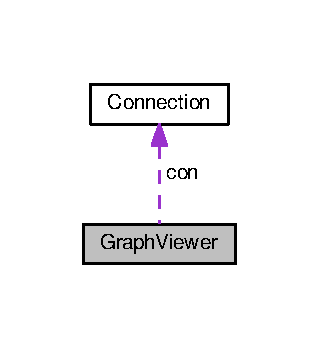
\includegraphics[width=153pt]{classGraphViewer__coll__graph}
\end{center}
\end{figure}
\subsection*{Public Member Functions}
\begin{DoxyCompactItemize}
\item 
\hyperlink{classGraphViewer_a8adc614f4fc290a3efcec7d7ceb1c58a}{Graph\+Viewer} (int \hyperlink{classGraphViewer_a5de27a1d20968b8494cd4bf5a4eb27e1}{width}, int \hyperlink{classGraphViewer_a9a1000e492a66ac4301c7135275690da}{height}, bool dynamic)
\item 
\hyperlink{classGraphViewer_ad9d7b1d8b4ba8ef18517eae0e68568a2}{Graph\+Viewer} (int \hyperlink{classGraphViewer_a5de27a1d20968b8494cd4bf5a4eb27e1}{width}, int \hyperlink{classGraphViewer_a9a1000e492a66ac4301c7135275690da}{height}, bool dynamic, int port\+\_\+n)
\item 
bool \hyperlink{classGraphViewer_ae5247dc66449dcd21fc5d531bbbaddfa}{create\+Window} (int \hyperlink{classGraphViewer_a5de27a1d20968b8494cd4bf5a4eb27e1}{width}, int \hyperlink{classGraphViewer_a9a1000e492a66ac4301c7135275690da}{height})
\item 
bool \hyperlink{classGraphViewer_a85990c1eaac7feed3950960d4bd2fd4c}{close\+Window} ()
\item 
bool \hyperlink{classGraphViewer_a5421e86ac76433876309236ba96e70a2}{add\+Node} (int id, int x, int y)
\item 
bool \hyperlink{classGraphViewer_ab9be856eb5f45284719a3bb119ec01ea}{add\+Node} (int id)
\item 
bool \hyperlink{classGraphViewer_aad0c1448c37f744209ffb671f1bd0015}{add\+Edge} (int id, int v1, int v2, int edge\+Type)
\item 
bool \hyperlink{classGraphViewer_a0c418639bb911eb827cabf895915f775}{remove\+Node} (int id)
\item 
bool \hyperlink{classGraphViewer_a9a8ee68c7c12b373affbe4069dd95d72}{remove\+Edge} (int id)
\item 
bool \hyperlink{classGraphViewer_ac25d7d007022fda16799808ba136e909}{set\+Vertex\+Label} (int id, string label)
\item 
bool \hyperlink{classGraphViewer_a447cca0064e785654c2105602c2961ca}{set\+Edge\+Label} (int id, string label)
\item 
bool \hyperlink{classGraphViewer_a07ccc96707efae4aa5f3ced3dca015af}{set\+Edge\+Color} (int id, string color)
\item 
bool \hyperlink{classGraphViewer_a1698f1c6b3a8e7cabc7b7d7cf42fc7f0}{set\+Edge\+Dashed} (int id, bool dashed)
\item 
bool \hyperlink{classGraphViewer_a8b542d7e09e81a45a74760c19233beb0}{set\+Vertex\+Color} (int id, string color)
\item 
bool \hyperlink{classGraphViewer_ae930dfdfcdeb7a871eefb6028d74b9f9}{set\+Vertex\+Size} (int id, int size)
\item 
bool \hyperlink{classGraphViewer_a02d5f7393eab9a2d1b66719039597a64}{set\+Vertex\+Icon} (int id, string filepath)
\item 
bool \hyperlink{classGraphViewer_a07f598272fe3515455eab13be749604a}{set\+Edge\+Thickness} (int id, int thickness)
\item 
bool \hyperlink{classGraphViewer_ac211de009a0afe2e6d44f4f8d030a2cc}{set\+Edge\+Weight} (int id, int weight)
\item 
bool \hyperlink{classGraphViewer_a69eb065145063e4dea41961e92e35c8e}{set\+Edge\+Flow} (int id, int flow)
\item 
bool \hyperlink{classGraphViewer_a08f362be0e682d91e7506dca8caae1b8}{define\+Edge\+Curved} (bool curved)
\item 
bool \hyperlink{classGraphViewer_a4102580b69826ba83251ef7bb262f8be}{define\+Edge\+Color} (string color)
\item 
bool \hyperlink{classGraphViewer_af785279b5c204df0e274b20c36276fc3}{define\+Edge\+Dashed} (bool dashed)
\item 
bool \hyperlink{classGraphViewer_a76de8676b7a93d72af514b84cdaa4d21}{define\+Vertex\+Color} (string color)
\item 
bool \hyperlink{classGraphViewer_ac4b2a9fec74d38e64088aa79ca4b7d9b}{define\+Vertex\+Size} (int size)
\item 
bool \hyperlink{classGraphViewer_af1adb6a361457187a820e01dcf0a34b7}{define\+Vertex\+Icon} (string filepath)
\item 
bool \hyperlink{classGraphViewer_a02437b5fecd8b90de24436068312d593}{set\+Background} (string path)
\item 
bool \hyperlink{classGraphViewer_a3009a66958686ccb7e78b68e37c3c423}{rearrange} ()
\end{DoxyCompactItemize}
\subsection*{Static Public Attributes}
\begin{DoxyCompactItemize}
\item 
static short \hyperlink{classGraphViewer_a89d0abe75f41feededc49497cc514342}{port} = 7772
\end{DoxyCompactItemize}
\subsection*{Private Member Functions}
\begin{DoxyCompactItemize}
\item 
void \hyperlink{classGraphViewer_a1ce9dff4903c650d3b2d33a3ef1d1f61}{initialize} (int, int, bool, int)
\end{DoxyCompactItemize}
\subsection*{Private Attributes}
\begin{DoxyCompactItemize}
\item 
int \hyperlink{classGraphViewer_a5de27a1d20968b8494cd4bf5a4eb27e1}{width}
\item 
int \hyperlink{classGraphViewer_a9a1000e492a66ac4301c7135275690da}{height}
\item 
bool \hyperlink{classGraphViewer_a9d9947154bc63354c6d02a0680aad952}{is\+Dynamic}
\item 
\hyperlink{classConnection}{Connection} $\ast$ \hyperlink{classGraphViewer_a14a206f78c242e739e0908b06070ba4d}{con}
\end{DoxyCompactItemize}


\subsection{Detailed Description}
Classe que guarda o grafo e o representa. Todas as suas funções retornam um booleano a indicar se a sua execução decorreu ou não com sucesso. 

\subsection{Constructor \& Destructor Documentation}
\index{Graph\+Viewer@{Graph\+Viewer}!Graph\+Viewer@{Graph\+Viewer}}
\index{Graph\+Viewer@{Graph\+Viewer}!Graph\+Viewer@{Graph\+Viewer}}
\subsubsection[{\texorpdfstring{Graph\+Viewer(int width, int height, bool dynamic)}{GraphViewer(int width, int height, bool dynamic)}}]{\setlength{\rightskip}{0pt plus 5cm}Graph\+Viewer\+::\+Graph\+Viewer (
\begin{DoxyParamCaption}
\item[{int}]{width, }
\item[{int}]{height, }
\item[{bool}]{dynamic}
\end{DoxyParamCaption}
)}\hypertarget{classGraphViewer_a8adc614f4fc290a3efcec7d7ceb1c58a}{}\label{classGraphViewer_a8adc614f4fc290a3efcec7d7ceb1c58a}
Construtor que cria um novo grafo e atribui automaticamente a porta. Exemplo\+: \hyperlink{classGraphViewer}{Graph\+Viewer} $\ast$gv = new \hyperlink{classGraphViewer}{Graph\+Viewer(600, 600, true)}; instancia um grafo 600x600, onde a posição dos nós é determinada automaticamente.


\begin{DoxyParams}{Parameters}
{\em width} & Inteiro que representa a lagura da área do grafo. \\
\hline
{\em height} & Inteiro que representa a altura da área do grafo. \\
\hline
{\em dynamic} & Booleano que determina se a localização dos nós é automaticamente. determinado pelo programa (true) ou se deve ser determinado pelo utilizador (false). \\
\hline
\end{DoxyParams}
\index{Graph\+Viewer@{Graph\+Viewer}!Graph\+Viewer@{Graph\+Viewer}}
\index{Graph\+Viewer@{Graph\+Viewer}!Graph\+Viewer@{Graph\+Viewer}}
\subsubsection[{\texorpdfstring{Graph\+Viewer(int width, int height, bool dynamic, int port\+\_\+n)}{GraphViewer(int width, int height, bool dynamic, int port_n)}}]{\setlength{\rightskip}{0pt plus 5cm}Graph\+Viewer\+::\+Graph\+Viewer (
\begin{DoxyParamCaption}
\item[{int}]{width, }
\item[{int}]{height, }
\item[{bool}]{dynamic, }
\item[{int}]{port\+\_\+n}
\end{DoxyParamCaption}
)}\hypertarget{classGraphViewer_ad9d7b1d8b4ba8ef18517eae0e68568a2}{}\label{classGraphViewer_ad9d7b1d8b4ba8ef18517eae0e68568a2}
Construtor que cria um novo grafo, utilizando uma porta especificada pelo utilizador para a ligação.

Exemplo\+: \hyperlink{classGraphViewer}{Graph\+Viewer} $\ast$gv = new \hyperlink{classGraphViewer}{Graph\+Viewer(600, 600, false, 3000)}; instancia um grafo 600x600, onde a posição dos nós é determinada pelo utilizador (usando a versão de add\+Node onde se pode especificar as coordenadas), sendo que a porta a usar para a comunicação é a 3000.


\begin{DoxyParams}{Parameters}
{\em width} & Inteiro que representa a lagura da área do grafo. \\
\hline
{\em height} & Inteiro que representa a altura da área do grafo. \\
\hline
{\em dynamic} & Booleano que determina se a localização dos nós é automaticamente. determinado pelo programa (true) ou se deve ser determinado pelo utilizador (false). \\
\hline
{\em port\+\_\+n} & Inteiro que determina a porta a utilizar. Deve-\/se ter cuidado para não utilizar uma porta já usada por outro programa ou pelo sistema. \\
\hline
\end{DoxyParams}


\subsection{Member Function Documentation}
\index{Graph\+Viewer@{Graph\+Viewer}!add\+Edge@{add\+Edge}}
\index{add\+Edge@{add\+Edge}!Graph\+Viewer@{Graph\+Viewer}}
\subsubsection[{\texorpdfstring{add\+Edge(int id, int v1, int v2, int edge\+Type)}{addEdge(int id, int v1, int v2, int edgeType)}}]{\setlength{\rightskip}{0pt plus 5cm}bool Graph\+Viewer\+::add\+Edge (
\begin{DoxyParamCaption}
\item[{int}]{id, }
\item[{int}]{v1, }
\item[{int}]{v2, }
\item[{int}]{edge\+Type}
\end{DoxyParamCaption}
)}\hypertarget{classGraphViewer_aad0c1448c37f744209ffb671f1bd0015}{}\label{classGraphViewer_aad0c1448c37f744209ffb671f1bd0015}
Acrescenta uma aresta à representação do grafo. Exemplo, para um apontador gv onde foi instanciada a classe \hyperlink{classGraphViewer}{Graph\+Viewer}\+: gv-\/$>$add\+Edge(0, 1, 2, Edge\+Type\+::\+U\+N\+D\+I\+R\+E\+C\+T\+E\+D); adiciona uma aresta não-\/dirigida com ID 0 que liga os nós com os I\+Ds 1 e 2


\begin{DoxyParams}{Parameters}
{\em id} & Identificador único da aresta. \\
\hline
{\em v1} & Identificador único do nó de origem da aresta. \\
\hline
{\em v2} & Identificador único do nó de destino da aresta. \\
\hline
{\em edge\+Type} & \hyperlink{classEdgeType_a903017a534f2818c2d17145e4ae0321c}{Edge\+Type.\+D\+I\+R\+E\+C\+T\+ED} caso a aresta seja unidirecional ou \hyperlink{classEdgeType_a6533cc56d05c288a550b9980b66c9317}{Edge\+Type.\+U\+N\+D\+I\+R\+E\+C\+T\+ED} caso a aresta seja bidirecional. \\
\hline
\end{DoxyParams}
\index{Graph\+Viewer@{Graph\+Viewer}!add\+Node@{add\+Node}}
\index{add\+Node@{add\+Node}!Graph\+Viewer@{Graph\+Viewer}}
\subsubsection[{\texorpdfstring{add\+Node(int id, int x, int y)}{addNode(int id, int x, int y)}}]{\setlength{\rightskip}{0pt plus 5cm}bool Graph\+Viewer\+::add\+Node (
\begin{DoxyParamCaption}
\item[{int}]{id, }
\item[{int}]{x, }
\item[{int}]{y}
\end{DoxyParamCaption}
)}\hypertarget{classGraphViewer_a5421e86ac76433876309236ba96e70a2}{}\label{classGraphViewer_a5421e86ac76433876309236ba96e70a2}
Acrescenta um nó à representação do grafo, numa posição específica, irrelevante se o grafo for dinâmico. Exemplo, para um apontador gv onde foi instanciada a classe \hyperlink{classGraphViewer}{Graph\+Viewer} com is\+Dynamic = false\+: gv-\/$>$add\+Node(0, 1, 2); adiciona um nó com ID 0 na posição (x, y) = (1, 2)


\begin{DoxyParams}{Parameters}
{\em id} & Identificador único do nó. \\
\hline
{\em x} & Posição horizontal do nó. \\
\hline
{\em y} & Posição vertical do nó. \\
\hline
\end{DoxyParams}
\index{Graph\+Viewer@{Graph\+Viewer}!add\+Node@{add\+Node}}
\index{add\+Node@{add\+Node}!Graph\+Viewer@{Graph\+Viewer}}
\subsubsection[{\texorpdfstring{add\+Node(int id)}{addNode(int id)}}]{\setlength{\rightskip}{0pt plus 5cm}bool Graph\+Viewer\+::add\+Node (
\begin{DoxyParamCaption}
\item[{int}]{id}
\end{DoxyParamCaption}
)}\hypertarget{classGraphViewer_ab9be856eb5f45284719a3bb119ec01ea}{}\label{classGraphViewer_ab9be856eb5f45284719a3bb119ec01ea}
Acrescenta um nó à representação do grafo, numa posição ao critério do programa. Só pode ser usado se o grafo for dinâmico, ou seja, se as posições de todos os nós forem atribuídas automaticamente. Caso contrário, não adiciona o nó. Exemplo, para um apontador gv onde foi instanciada a classe \hyperlink{classGraphViewer}{Graph\+Viewer} com is\+Dynamic = true\+: gv-\/$>$add\+Node(0); adiciona um nó com ID 0


\begin{DoxyParams}{Parameters}
{\em id} & Identificador único do nó. \\
\hline
\end{DoxyParams}
\index{Graph\+Viewer@{Graph\+Viewer}!close\+Window@{close\+Window}}
\index{close\+Window@{close\+Window}!Graph\+Viewer@{Graph\+Viewer}}
\subsubsection[{\texorpdfstring{close\+Window()}{closeWindow()}}]{\setlength{\rightskip}{0pt plus 5cm}bool Graph\+Viewer\+::close\+Window (
\begin{DoxyParamCaption}
{}
\end{DoxyParamCaption}
)}\hypertarget{classGraphViewer_a85990c1eaac7feed3950960d4bd2fd4c}{}\label{classGraphViewer_a85990c1eaac7feed3950960d4bd2fd4c}
Fecha a janela a ser utilizada para visualização. \index{Graph\+Viewer@{Graph\+Viewer}!create\+Window@{create\+Window}}
\index{create\+Window@{create\+Window}!Graph\+Viewer@{Graph\+Viewer}}
\subsubsection[{\texorpdfstring{create\+Window(int width, int height)}{createWindow(int width, int height)}}]{\setlength{\rightskip}{0pt plus 5cm}bool Graph\+Viewer\+::create\+Window (
\begin{DoxyParamCaption}
\item[{int}]{width, }
\item[{int}]{height}
\end{DoxyParamCaption}
)}\hypertarget{classGraphViewer_ae5247dc66449dcd21fc5d531bbbaddfa}{}\label{classGraphViewer_ae5247dc66449dcd21fc5d531bbbaddfa}
Função que cria a janela para visualização. Exemplo, para um apontador gv onde foi instanciada a classe \hyperlink{classGraphViewer}{Graph\+Viewer}\+: gv-\/$>$create\+Window(600, 600); abre uma janela 600x600 onde mostra o grafo.


\begin{DoxyParams}{Parameters}
{\em width} & Largura da janela a criar. \\
\hline
{\em height} & Altura da janela a criar. \\
\hline
\end{DoxyParams}
\index{Graph\+Viewer@{Graph\+Viewer}!define\+Edge\+Color@{define\+Edge\+Color}}
\index{define\+Edge\+Color@{define\+Edge\+Color}!Graph\+Viewer@{Graph\+Viewer}}
\subsubsection[{\texorpdfstring{define\+Edge\+Color(string color)}{defineEdgeColor(string color)}}]{\setlength{\rightskip}{0pt plus 5cm}bool Graph\+Viewer\+::define\+Edge\+Color (
\begin{DoxyParamCaption}
\item[{string}]{color}
\end{DoxyParamCaption}
)}\hypertarget{classGraphViewer_a4102580b69826ba83251ef7bb262f8be}{}\label{classGraphViewer_a4102580b69826ba83251ef7bb262f8be}
Função que define a cor global das arestas. Exemplo, para um apontador gv onde foi instanciada a classe \hyperlink{classGraphViewer}{Graph\+Viewer}\+: gv-\/$>$define\+Edge\+Color(\+G\+R\+A\+Y); modifica a cor por defeito das arestas para cinzento


\begin{DoxyParams}{Parameters}
{\em color} & Nova cor das arestas, utilizar as constantes definidas no \hyperlink{graphviewer_8h}{graphviewer.\+h} para conveniência. \\
\hline
\end{DoxyParams}
\index{Graph\+Viewer@{Graph\+Viewer}!define\+Edge\+Curved@{define\+Edge\+Curved}}
\index{define\+Edge\+Curved@{define\+Edge\+Curved}!Graph\+Viewer@{Graph\+Viewer}}
\subsubsection[{\texorpdfstring{define\+Edge\+Curved(bool curved)}{defineEdgeCurved(bool curved)}}]{\setlength{\rightskip}{0pt plus 5cm}bool Graph\+Viewer\+::define\+Edge\+Curved (
\begin{DoxyParamCaption}
\item[{bool}]{curved}
\end{DoxyParamCaption}
)}\hypertarget{classGraphViewer_a08f362be0e682d91e7506dca8caae1b8}{}\label{classGraphViewer_a08f362be0e682d91e7506dca8caae1b8}
Função que define se as arestas do grafo serão desenhadas como curvas ou retas. Exemplo, para um apontador gv onde foi instanciada a classe \hyperlink{classGraphViewer}{Graph\+Viewer}\+: gv-\/$>$define\+Edge\+Curved(false); faz com que as arestas sejam desenhadas como retas


\begin{DoxyParams}{Parameters}
{\em curved} & Booleano que representa se as arestas serão curvas (true) ou retas (false), sendo o valor por defeito é true. \\
\hline
\end{DoxyParams}
\index{Graph\+Viewer@{Graph\+Viewer}!define\+Edge\+Dashed@{define\+Edge\+Dashed}}
\index{define\+Edge\+Dashed@{define\+Edge\+Dashed}!Graph\+Viewer@{Graph\+Viewer}}
\subsubsection[{\texorpdfstring{define\+Edge\+Dashed(bool dashed)}{defineEdgeDashed(bool dashed)}}]{\setlength{\rightskip}{0pt plus 5cm}bool Graph\+Viewer\+::define\+Edge\+Dashed (
\begin{DoxyParamCaption}
\item[{bool}]{dashed}
\end{DoxyParamCaption}
)}\hypertarget{classGraphViewer_af785279b5c204df0e274b20c36276fc3}{}\label{classGraphViewer_af785279b5c204df0e274b20c36276fc3}
Função que define globalmente se as arestas são desenhadas, ou não, a tracejado. Exemplo, para um apontador gv onde foi instanciada a classe \hyperlink{classGraphViewer}{Graph\+Viewer}\+: gv-\/$>$define\+Edge\+Dashed(true); faz com que por defeito as arestas sejam desenhadas a tracejado


\begin{DoxyParams}{Parameters}
{\em dashed} & Booleano que representa se as arestas vão estar, ou não, todas a tracejado (o valor por defeito é false). \\
\hline
\end{DoxyParams}
\index{Graph\+Viewer@{Graph\+Viewer}!define\+Vertex\+Color@{define\+Vertex\+Color}}
\index{define\+Vertex\+Color@{define\+Vertex\+Color}!Graph\+Viewer@{Graph\+Viewer}}
\subsubsection[{\texorpdfstring{define\+Vertex\+Color(string color)}{defineVertexColor(string color)}}]{\setlength{\rightskip}{0pt plus 5cm}bool Graph\+Viewer\+::define\+Vertex\+Color (
\begin{DoxyParamCaption}
\item[{string}]{color}
\end{DoxyParamCaption}
)}\hypertarget{classGraphViewer_a76de8676b7a93d72af514b84cdaa4d21}{}\label{classGraphViewer_a76de8676b7a93d72af514b84cdaa4d21}
Função que define a cor global dos nós. Exemplo, para um apontador gv onde foi instanciada a classe \hyperlink{classGraphViewer}{Graph\+Viewer}\+: gv-\/$>$define\+Vertex\+Color(\+R\+E\+D); modifica a cor por defeito dos nós para vermelho


\begin{DoxyParams}{Parameters}
{\em color} & Nova cor dos nós, utilizar as constantes definidas no \hyperlink{graphviewer_8h}{graphviewer.\+h} para conveniência. \\
\hline
\end{DoxyParams}
\index{Graph\+Viewer@{Graph\+Viewer}!define\+Vertex\+Icon@{define\+Vertex\+Icon}}
\index{define\+Vertex\+Icon@{define\+Vertex\+Icon}!Graph\+Viewer@{Graph\+Viewer}}
\subsubsection[{\texorpdfstring{define\+Vertex\+Icon(string filepath)}{defineVertexIcon(string filepath)}}]{\setlength{\rightskip}{0pt plus 5cm}bool Graph\+Viewer\+::define\+Vertex\+Icon (
\begin{DoxyParamCaption}
\item[{string}]{filepath}
\end{DoxyParamCaption}
)}\hypertarget{classGraphViewer_af1adb6a361457187a820e01dcf0a34b7}{}\label{classGraphViewer_af1adb6a361457187a820e01dcf0a34b7}
Função que define um ícone para um nó. Exemplo, para um apontador gv onde foi instanciada a classe \hyperlink{classGraphViewer}{Graph\+Viewer}\+: gv-\/$>$define\+Vertex\+Icon(\char`\"{}icon.\+gif\char`\"{}); faz com que por defeito os nós, quando desenhados, não sejam um círculo, mas sim a imagem icon.\+gif


\begin{DoxyParams}{Parameters}
{\em filepath} & Caminho do ficheiro a utilizar como novo ícone do nó. \\
\hline
\end{DoxyParams}
\index{Graph\+Viewer@{Graph\+Viewer}!define\+Vertex\+Size@{define\+Vertex\+Size}}
\index{define\+Vertex\+Size@{define\+Vertex\+Size}!Graph\+Viewer@{Graph\+Viewer}}
\subsubsection[{\texorpdfstring{define\+Vertex\+Size(int size)}{defineVertexSize(int size)}}]{\setlength{\rightskip}{0pt plus 5cm}bool Graph\+Viewer\+::define\+Vertex\+Size (
\begin{DoxyParamCaption}
\item[{int}]{size}
\end{DoxyParamCaption}
)}\hypertarget{classGraphViewer_ac4b2a9fec74d38e64088aa79ca4b7d9b}{}\label{classGraphViewer_ac4b2a9fec74d38e64088aa79ca4b7d9b}
Função que define o tamanho global dos nós. Exemplo, para um apontador gv onde foi instanciada a classe \hyperlink{classGraphViewer}{Graph\+Viewer}\+: gv-\/$>$define\+Vertex\+Size(20); modifica o tamanho por defeito dos nós para 20


\begin{DoxyParams}{Parameters}
{\em size} & Nova cor dos nós, utilizar as constantes definidas no \hyperlink{graphviewer_8h}{graphviewer.\+h} para conveniência. \\
\hline
\end{DoxyParams}
\index{Graph\+Viewer@{Graph\+Viewer}!initialize@{initialize}}
\index{initialize@{initialize}!Graph\+Viewer@{Graph\+Viewer}}
\subsubsection[{\texorpdfstring{initialize(int, int, bool, int)}{initialize(int, int, bool, int)}}]{\setlength{\rightskip}{0pt plus 5cm}void Graph\+Viewer\+::initialize (
\begin{DoxyParamCaption}
\item[{int}]{width, }
\item[{int}]{height, }
\item[{bool}]{dynamic, }
\item[{int}]{port\+\_\+n}
\end{DoxyParamCaption}
)\hspace{0.3cm}{\ttfamily [private]}}\hypertarget{classGraphViewer_a1ce9dff4903c650d3b2d33a3ef1d1f61}{}\label{classGraphViewer_a1ce9dff4903c650d3b2d33a3ef1d1f61}
\index{Graph\+Viewer@{Graph\+Viewer}!rearrange@{rearrange}}
\index{rearrange@{rearrange}!Graph\+Viewer@{Graph\+Viewer}}
\subsubsection[{\texorpdfstring{rearrange()}{rearrange()}}]{\setlength{\rightskip}{0pt plus 5cm}bool Graph\+Viewer\+::rearrange (
\begin{DoxyParamCaption}
{}
\end{DoxyParamCaption}
)}\hypertarget{classGraphViewer_a3009a66958686ccb7e78b68e37c3c423}{}\label{classGraphViewer_a3009a66958686ccb7e78b68e37c3c423}
Função que actualiza a visualização do grafo. \index{Graph\+Viewer@{Graph\+Viewer}!remove\+Edge@{remove\+Edge}}
\index{remove\+Edge@{remove\+Edge}!Graph\+Viewer@{Graph\+Viewer}}
\subsubsection[{\texorpdfstring{remove\+Edge(int id)}{removeEdge(int id)}}]{\setlength{\rightskip}{0pt plus 5cm}bool Graph\+Viewer\+::remove\+Edge (
\begin{DoxyParamCaption}
\item[{int}]{id}
\end{DoxyParamCaption}
)}\hypertarget{classGraphViewer_a9a8ee68c7c12b373affbe4069dd95d72}{}\label{classGraphViewer_a9a8ee68c7c12b373affbe4069dd95d72}
Remove uma aresta da representação do grafo. Exemplo, para um apontador gv onde foi instanciada a classe \hyperlink{classGraphViewer}{Graph\+Viewer}\+: gv-\/$>$remove\+Edge(0) remove a aresta com ID 0


\begin{DoxyParams}{Parameters}
{\em id} & Identificador único da aresta a remover. \\
\hline
\end{DoxyParams}
\index{Graph\+Viewer@{Graph\+Viewer}!remove\+Node@{remove\+Node}}
\index{remove\+Node@{remove\+Node}!Graph\+Viewer@{Graph\+Viewer}}
\subsubsection[{\texorpdfstring{remove\+Node(int id)}{removeNode(int id)}}]{\setlength{\rightskip}{0pt plus 5cm}bool Graph\+Viewer\+::remove\+Node (
\begin{DoxyParamCaption}
\item[{int}]{id}
\end{DoxyParamCaption}
)}\hypertarget{classGraphViewer_a0c418639bb911eb827cabf895915f775}{}\label{classGraphViewer_a0c418639bb911eb827cabf895915f775}
Remove um nó da representação do grafo e todas as arestas ligadas a este. Exemplo, para um apontador gv onde foi instanciada a classe \hyperlink{classGraphViewer}{Graph\+Viewer}\+: gv-\/$>$remove\+Node(0) remove o nó com ID 0


\begin{DoxyParams}{Parameters}
{\em id} & Identificador único do nó a a remover. \\
\hline
\end{DoxyParams}
\index{Graph\+Viewer@{Graph\+Viewer}!set\+Background@{set\+Background}}
\index{set\+Background@{set\+Background}!Graph\+Viewer@{Graph\+Viewer}}
\subsubsection[{\texorpdfstring{set\+Background(string path)}{setBackground(string path)}}]{\setlength{\rightskip}{0pt plus 5cm}bool Graph\+Viewer\+::set\+Background (
\begin{DoxyParamCaption}
\item[{string}]{path}
\end{DoxyParamCaption}
)}\hypertarget{classGraphViewer_a02437b5fecd8b90de24436068312d593}{}\label{classGraphViewer_a02437b5fecd8b90de24436068312d593}
Função que altera a imagem de fundo do grafo. Exemplo, para um apontador gv onde foi instanciada a classe \hyperlink{classGraphViewer}{Graph\+Viewer}\+: gv-\/$>$set\+Back\+Ground(\char`\"{}fundo.\+png\char`\"{}); faz com que o fundo da janela seja a imagem fundo.\+png, em vez de cinzento


\begin{DoxyParams}{Parameters}
{\em path} & Caminho para o ficheiro com a imagem. \\
\hline
\end{DoxyParams}
\index{Graph\+Viewer@{Graph\+Viewer}!set\+Edge\+Color@{set\+Edge\+Color}}
\index{set\+Edge\+Color@{set\+Edge\+Color}!Graph\+Viewer@{Graph\+Viewer}}
\subsubsection[{\texorpdfstring{set\+Edge\+Color(int id, string color)}{setEdgeColor(int id, string color)}}]{\setlength{\rightskip}{0pt plus 5cm}bool Graph\+Viewer\+::set\+Edge\+Color (
\begin{DoxyParamCaption}
\item[{int}]{id, }
\item[{string}]{color}
\end{DoxyParamCaption}
)}\hypertarget{classGraphViewer_a07ccc96707efae4aa5f3ced3dca015af}{}\label{classGraphViewer_a07ccc96707efae4aa5f3ced3dca015af}
Função que define a cor de uma aresta. Exemplo, para um apontador gv onde foi instanciada a classe \hyperlink{classGraphViewer}{Graph\+Viewer}\+: gv-\/$>$set\+Edge\+Color(0, B\+L\+U\+E); modifica a cor da aresta com ID 0 para azul


\begin{DoxyParams}{Parameters}
{\em id} & Identificador único da aresta com a cor a alterar. \\
\hline
{\em color} & Nova cor da aresta, utilizar as constantes definidas no \hyperlink{graphviewer_8h}{graphviewer.\+h} para conveniência. \\
\hline
\end{DoxyParams}
\index{Graph\+Viewer@{Graph\+Viewer}!set\+Edge\+Dashed@{set\+Edge\+Dashed}}
\index{set\+Edge\+Dashed@{set\+Edge\+Dashed}!Graph\+Viewer@{Graph\+Viewer}}
\subsubsection[{\texorpdfstring{set\+Edge\+Dashed(int id, bool dashed)}{setEdgeDashed(int id, bool dashed)}}]{\setlength{\rightskip}{0pt plus 5cm}bool Graph\+Viewer\+::set\+Edge\+Dashed (
\begin{DoxyParamCaption}
\item[{int}]{id, }
\item[{bool}]{dashed}
\end{DoxyParamCaption}
)}\hypertarget{classGraphViewer_a1698f1c6b3a8e7cabc7b7d7cf42fc7f0}{}\label{classGraphViewer_a1698f1c6b3a8e7cabc7b7d7cf42fc7f0}
Função que define se uma aresta é desenhada, ou não, a tracejado. Exemplo, para um apontador gv onde foi instanciada a classe \hyperlink{classGraphViewer}{Graph\+Viewer}\+: gv-\/$>$set\+Edge\+Dashed(0, false); faz com que a aresta com ID 0 seja desenhada a traço contínuo


\begin{DoxyParams}{Parameters}
{\em id} & Identificador único da aresta com a cor a alterar. \\
\hline
{\em dashed} & Nova cor da aresta, utilizar as constantes definidas no \hyperlink{graphviewer_8h}{graphviewer.\+h} para conveniência. \\
\hline
\end{DoxyParams}
\index{Graph\+Viewer@{Graph\+Viewer}!set\+Edge\+Flow@{set\+Edge\+Flow}}
\index{set\+Edge\+Flow@{set\+Edge\+Flow}!Graph\+Viewer@{Graph\+Viewer}}
\subsubsection[{\texorpdfstring{set\+Edge\+Flow(int id, int flow)}{setEdgeFlow(int id, int flow)}}]{\setlength{\rightskip}{0pt plus 5cm}bool Graph\+Viewer\+::set\+Edge\+Flow (
\begin{DoxyParamCaption}
\item[{int}]{id, }
\item[{int}]{flow}
\end{DoxyParamCaption}
)}\hypertarget{classGraphViewer_a69eb065145063e4dea41961e92e35c8e}{}\label{classGraphViewer_a69eb065145063e4dea41961e92e35c8e}
Função que define o fluxo de uma aresta na representação do grafo, a ser visualizado como f\+: valor\+\_\+do\+\_\+fluxo, precedido pelo peso e seguido por texto definido pelo utilizador. Exemplo, para um apontador gv onde foi instanciada a classe \hyperlink{classGraphViewer}{Graph\+Viewer}\+: gv-\/$>$set\+Edge\+Flow(0, 20); modifica o fluxo da aresta com ID 0 para 20


\begin{DoxyParams}{Parameters}
{\em id} & Identificador único da aresta a modificar. \\
\hline
{\em flow} & Fluxo associado à aresta. \\
\hline
\end{DoxyParams}
\index{Graph\+Viewer@{Graph\+Viewer}!set\+Edge\+Label@{set\+Edge\+Label}}
\index{set\+Edge\+Label@{set\+Edge\+Label}!Graph\+Viewer@{Graph\+Viewer}}
\subsubsection[{\texorpdfstring{set\+Edge\+Label(int id, string label)}{setEdgeLabel(int id, string label)}}]{\setlength{\rightskip}{0pt plus 5cm}bool Graph\+Viewer\+::set\+Edge\+Label (
\begin{DoxyParamCaption}
\item[{int}]{id, }
\item[{string}]{label}
\end{DoxyParamCaption}
)}\hypertarget{classGraphViewer_a447cca0064e785654c2105602c2961ca}{}\label{classGraphViewer_a447cca0064e785654c2105602c2961ca}
Função que define o texto de uma aresta. Exemplo, para um apontador gv onde foi instanciada a classe \hyperlink{classGraphViewer}{Graph\+Viewer}\+: gv-\/$>$set\+Edge\+Label(0, \char`\"{}\+Isto é uma aresta\char`\"{}); adiciona o texto \char`\"{}\+Isto é uma aresta\char`\"{} à aresta com ID 0


\begin{DoxyParams}{Parameters}
{\em id} & Identificador único da aresta com o texto a alterar. \\
\hline
{\em label} & Novo texto da aresta. \\
\hline
\end{DoxyParams}
\index{Graph\+Viewer@{Graph\+Viewer}!set\+Edge\+Thickness@{set\+Edge\+Thickness}}
\index{set\+Edge\+Thickness@{set\+Edge\+Thickness}!Graph\+Viewer@{Graph\+Viewer}}
\subsubsection[{\texorpdfstring{set\+Edge\+Thickness(int id, int thickness)}{setEdgeThickness(int id, int thickness)}}]{\setlength{\rightskip}{0pt plus 5cm}bool Graph\+Viewer\+::set\+Edge\+Thickness (
\begin{DoxyParamCaption}
\item[{int}]{id, }
\item[{int}]{thickness}
\end{DoxyParamCaption}
)}\hypertarget{classGraphViewer_a07f598272fe3515455eab13be749604a}{}\label{classGraphViewer_a07f598272fe3515455eab13be749604a}
Função que define a espessura de uma aresta. Exemplo, para um apontador gv onde foi instanciada a classe \hyperlink{classGraphViewer}{Graph\+Viewer}\+: gv-\/$>$set\+Edge\+Thickness(0, 20); modifica a espessura da aresta com ID 0 para 20


\begin{DoxyParams}{Parameters}
{\em id} & Identificador único da aresta com a espessura a alterar. \\
\hline
{\em thickness} & Nova espessura da aresta, sendo que por base, as arestas são criadas com a espessura de 1. \\
\hline
\end{DoxyParams}
\index{Graph\+Viewer@{Graph\+Viewer}!set\+Edge\+Weight@{set\+Edge\+Weight}}
\index{set\+Edge\+Weight@{set\+Edge\+Weight}!Graph\+Viewer@{Graph\+Viewer}}
\subsubsection[{\texorpdfstring{set\+Edge\+Weight(int id, int weight)}{setEdgeWeight(int id, int weight)}}]{\setlength{\rightskip}{0pt plus 5cm}bool Graph\+Viewer\+::set\+Edge\+Weight (
\begin{DoxyParamCaption}
\item[{int}]{id, }
\item[{int}]{weight}
\end{DoxyParamCaption}
)}\hypertarget{classGraphViewer_ac211de009a0afe2e6d44f4f8d030a2cc}{}\label{classGraphViewer_ac211de009a0afe2e6d44f4f8d030a2cc}
Função que define o peso de uma aresta na representação do grafo, a ser visualizado como w\+: valor\+\_\+do\+\_\+peso, seguido de qualquer outro texto associado à aresta. Exemplo, para um apontador gv onde foi instanciada a classe \hyperlink{classGraphViewer}{Graph\+Viewer}\+: gv-\/$>$set\+Edge\+Weight(0, 20); modifica o peso da aresta com ID 0 para 20


\begin{DoxyParams}{Parameters}
{\em id} & Identificador único da aresta a modificar. \\
\hline
{\em weight} & Peso associado à aresta. \\
\hline
\end{DoxyParams}
\index{Graph\+Viewer@{Graph\+Viewer}!set\+Vertex\+Color@{set\+Vertex\+Color}}
\index{set\+Vertex\+Color@{set\+Vertex\+Color}!Graph\+Viewer@{Graph\+Viewer}}
\subsubsection[{\texorpdfstring{set\+Vertex\+Color(int id, string color)}{setVertexColor(int id, string color)}}]{\setlength{\rightskip}{0pt plus 5cm}bool Graph\+Viewer\+::set\+Vertex\+Color (
\begin{DoxyParamCaption}
\item[{int}]{id, }
\item[{string}]{color}
\end{DoxyParamCaption}
)}\hypertarget{classGraphViewer_a8b542d7e09e81a45a74760c19233beb0}{}\label{classGraphViewer_a8b542d7e09e81a45a74760c19233beb0}
Função que define a cor de um nó. Exemplo, para um apontador gv onde foi instanciada a classe \hyperlink{classGraphViewer}{Graph\+Viewer}\+: gv-\/$>$set\+Vertex\+Color(0, G\+R\+E\+E\+N); modifica a cor do nó com ID 0 para verde


\begin{DoxyParams}{Parameters}
{\em id} & Identificador único do nó com a cor a alterar. \\
\hline
{\em color} & Nova cor do nó, utilizar as constantes definidas no \hyperlink{graphviewer_8h}{graphviewer.\+h} para conveniência. \\
\hline
\end{DoxyParams}
\index{Graph\+Viewer@{Graph\+Viewer}!set\+Vertex\+Icon@{set\+Vertex\+Icon}}
\index{set\+Vertex\+Icon@{set\+Vertex\+Icon}!Graph\+Viewer@{Graph\+Viewer}}
\subsubsection[{\texorpdfstring{set\+Vertex\+Icon(int id, string filepath)}{setVertexIcon(int id, string filepath)}}]{\setlength{\rightskip}{0pt plus 5cm}bool Graph\+Viewer\+::set\+Vertex\+Icon (
\begin{DoxyParamCaption}
\item[{int}]{id, }
\item[{string}]{filepath}
\end{DoxyParamCaption}
)}\hypertarget{classGraphViewer_a02d5f7393eab9a2d1b66719039597a64}{}\label{classGraphViewer_a02d5f7393eab9a2d1b66719039597a64}
Função que define um ícone para um nó. Exemplo, para um apontador gv onde foi instanciada a classe \hyperlink{classGraphViewer}{Graph\+Viewer}\+: gv-\/$>$set\+Vertex\+Icon(0, \char`\"{}icon.\+png\char`\"{}); faz com que o nó, quando desenhado, não seja um círculo, mas sim a imagem icon.\+png


\begin{DoxyParams}{Parameters}
{\em id} & Identificador único do nó com o ícone a alterar. \\
\hline
{\em filepath} & Caminho do ficheiro a utilizar como novo ícone do nó. \\
\hline
\end{DoxyParams}
\index{Graph\+Viewer@{Graph\+Viewer}!set\+Vertex\+Label@{set\+Vertex\+Label}}
\index{set\+Vertex\+Label@{set\+Vertex\+Label}!Graph\+Viewer@{Graph\+Viewer}}
\subsubsection[{\texorpdfstring{set\+Vertex\+Label(int id, string label)}{setVertexLabel(int id, string label)}}]{\setlength{\rightskip}{0pt plus 5cm}bool Graph\+Viewer\+::set\+Vertex\+Label (
\begin{DoxyParamCaption}
\item[{int}]{id, }
\item[{string}]{label}
\end{DoxyParamCaption}
)}\hypertarget{classGraphViewer_ac25d7d007022fda16799808ba136e909}{}\label{classGraphViewer_ac25d7d007022fda16799808ba136e909}
Função que define o texto de um nó. Exemplo, para um apontador gv onde foi instanciada a classe \hyperlink{classGraphViewer}{Graph\+Viewer}\+: gv-\/$>$set\+Vertex\+Label(0, \char`\"{}\+Isto é um nó\char`\"{}); adiciona o texto \char`\"{}\+Isto é um nó\char`\"{} ao nó com ID 0


\begin{DoxyParams}{Parameters}
{\em id} & Identificador único do nó com o texto a alterar. \\
\hline
{\em label} & Novo texto do nó. \\
\hline
\end{DoxyParams}
\index{Graph\+Viewer@{Graph\+Viewer}!set\+Vertex\+Size@{set\+Vertex\+Size}}
\index{set\+Vertex\+Size@{set\+Vertex\+Size}!Graph\+Viewer@{Graph\+Viewer}}
\subsubsection[{\texorpdfstring{set\+Vertex\+Size(int id, int size)}{setVertexSize(int id, int size)}}]{\setlength{\rightskip}{0pt plus 5cm}bool Graph\+Viewer\+::set\+Vertex\+Size (
\begin{DoxyParamCaption}
\item[{int}]{id, }
\item[{int}]{size}
\end{DoxyParamCaption}
)}\hypertarget{classGraphViewer_ae930dfdfcdeb7a871eefb6028d74b9f9}{}\label{classGraphViewer_ae930dfdfcdeb7a871eefb6028d74b9f9}
Função que define o tamanho de um nó. Exemplo, para um apontador gv onde foi instanciada a classe \hyperlink{classGraphViewer}{Graph\+Viewer}\+: gv-\/$>$set\+Vertex\+Size(0, 10); modifica o tamanho do nó com ID 0 para 40


\begin{DoxyParams}{Parameters}
{\em id} & Identificador único do nó com o tamanho a alterar. \\
\hline
{\em size} & Novo tamanho do nó. \\
\hline
\end{DoxyParams}


\subsection{Member Data Documentation}
\index{Graph\+Viewer@{Graph\+Viewer}!con@{con}}
\index{con@{con}!Graph\+Viewer@{Graph\+Viewer}}
\subsubsection[{\texorpdfstring{con}{con}}]{\setlength{\rightskip}{0pt plus 5cm}{\bf Connection}$\ast$ Graph\+Viewer\+::con\hspace{0.3cm}{\ttfamily [private]}}\hypertarget{classGraphViewer_a14a206f78c242e739e0908b06070ba4d}{}\label{classGraphViewer_a14a206f78c242e739e0908b06070ba4d}
\index{Graph\+Viewer@{Graph\+Viewer}!height@{height}}
\index{height@{height}!Graph\+Viewer@{Graph\+Viewer}}
\subsubsection[{\texorpdfstring{height}{height}}]{\setlength{\rightskip}{0pt plus 5cm}int Graph\+Viewer\+::height\hspace{0.3cm}{\ttfamily [private]}}\hypertarget{classGraphViewer_a9a1000e492a66ac4301c7135275690da}{}\label{classGraphViewer_a9a1000e492a66ac4301c7135275690da}
\index{Graph\+Viewer@{Graph\+Viewer}!is\+Dynamic@{is\+Dynamic}}
\index{is\+Dynamic@{is\+Dynamic}!Graph\+Viewer@{Graph\+Viewer}}
\subsubsection[{\texorpdfstring{is\+Dynamic}{isDynamic}}]{\setlength{\rightskip}{0pt plus 5cm}bool Graph\+Viewer\+::is\+Dynamic\hspace{0.3cm}{\ttfamily [private]}}\hypertarget{classGraphViewer_a9d9947154bc63354c6d02a0680aad952}{}\label{classGraphViewer_a9d9947154bc63354c6d02a0680aad952}
\index{Graph\+Viewer@{Graph\+Viewer}!port@{port}}
\index{port@{port}!Graph\+Viewer@{Graph\+Viewer}}
\subsubsection[{\texorpdfstring{port}{port}}]{\setlength{\rightskip}{0pt plus 5cm}short Graph\+Viewer\+::port = 7772\hspace{0.3cm}{\ttfamily [static]}}\hypertarget{classGraphViewer_a89d0abe75f41feededc49497cc514342}{}\label{classGraphViewer_a89d0abe75f41feededc49497cc514342}
Variável que guarda a próxima porta que o programa vai usar. O valor inicial é 7772. \index{Graph\+Viewer@{Graph\+Viewer}!width@{width}}
\index{width@{width}!Graph\+Viewer@{Graph\+Viewer}}
\subsubsection[{\texorpdfstring{width}{width}}]{\setlength{\rightskip}{0pt plus 5cm}int Graph\+Viewer\+::width\hspace{0.3cm}{\ttfamily [private]}}\hypertarget{classGraphViewer_a5de27a1d20968b8494cd4bf5a4eb27e1}{}\label{classGraphViewer_a5de27a1d20968b8494cd4bf5a4eb27e1}


The documentation for this class was generated from the following files\+:\begin{DoxyCompactItemize}
\item 
/home/amadeu/\+Desktop/\+Cal-\/2018/src/\hyperlink{graphviewer_8h}{graphviewer.\+h}\item 
/home/amadeu/\+Desktop/\+Cal-\/2018/src/\hyperlink{graphviewer_8cpp}{graphviewer.\+cpp}\end{DoxyCompactItemize}

\hypertarget{classInterface}{}\section{Interface Class Reference}
\label{classInterface}\index{Interface@{Interface}}


{\ttfamily \#include $<$Interface.\+h$>$}



Collaboration diagram for Interface\+:\nopagebreak
\begin{figure}[H]
\begin{center}
\leavevmode
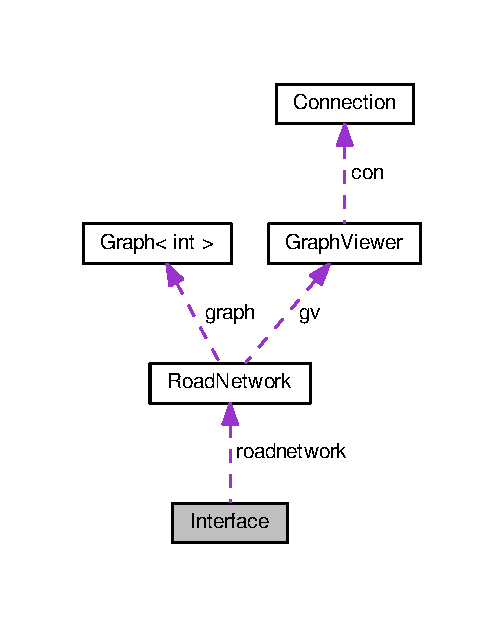
\includegraphics[width=242pt]{classInterface__coll__graph}
\end{center}
\end{figure}
\subsection*{Public Member Functions}
\begin{DoxyCompactItemize}
\item 
\hyperlink{classInterface_a4406d74c75bdfe150bf72be1f1cda8b1}{Interface} ()
\item 
virtual \hyperlink{classInterface_a19179888f29f18f1be54a3dfe98f68c0}{$\sim$\+Interface} ()
\item 
void \hyperlink{classInterface_a04428812c5138654aaed3c17bc8f7deb}{convert\+To\+GV} ()
\item 
void \hyperlink{classInterface_a8b09945f62fc12fb90de30046042efe3}{roads\+Blocked} ()
\item 
void \hyperlink{classInterface_ae4cad587f14fd078f118858ef2f73015}{calculate\+Path} ()
\item 
void \hyperlink{classInterface_aec46d793b0a3ac1196dd61df896e154a}{show\+Map} ()
\item 
void \hyperlink{classInterface_a4134df58f667cd4d51f3666828cff73b}{update\+Map} ()
\item 
void \hyperlink{classInterface_a3afcfe1089d52a1359602dca26611657}{close\+Map\+Window} ()
\item 
void \hyperlink{classInterface_a3e043e9aa51fa1e16436d1a3247a9daa}{get\+All\+Cars\+Path} ()
\item 
void \hyperlink{classInterface_a2bbf8267df70e1aa4a225ab4ca17ff66}{remove\+Car} ()
\item 
void \hyperlink{classInterface_ac9d3a7f7dd91e5684e988942d1e62c6f}{return\+Menu} ()
\item 
void \hyperlink{classInterface_a7b37d708a88660698fc79f0e7bbedb95}{return\+Menu2} ()
\item 
void \hyperlink{classInterface_afa0a2e9fbced7c9451e2a3cddcd39d6a}{write\+Files} ()
\end{DoxyCompactItemize}
\subsection*{Private Attributes}
\begin{DoxyCompactItemize}
\item 
\hyperlink{classRoadNetwork}{Road\+Network} $\ast$ \hyperlink{classInterface_aae76b1bb86e685e441c21f5f5b68ef99}{roadnetwork}
\end{DoxyCompactItemize}


\subsection{Constructor \& Destructor Documentation}
\index{Interface@{Interface}!Interface@{Interface}}
\index{Interface@{Interface}!Interface@{Interface}}
\subsubsection[{\texorpdfstring{Interface()}{Interface()}}]{\setlength{\rightskip}{0pt plus 5cm}Interface\+::\+Interface (
\begin{DoxyParamCaption}
{}
\end{DoxyParamCaption}
)}\hypertarget{classInterface_a4406d74c75bdfe150bf72be1f1cda8b1}{}\label{classInterface_a4406d74c75bdfe150bf72be1f1cda8b1}
Construtor da classe \hyperlink{classInterface}{Interface} \index{Interface@{Interface}!````~Interface@{$\sim$\+Interface}}
\index{````~Interface@{$\sim$\+Interface}!Interface@{Interface}}
\subsubsection[{\texorpdfstring{$\sim$\+Interface()}{~Interface()}}]{\setlength{\rightskip}{0pt plus 5cm}Interface\+::$\sim$\+Interface (
\begin{DoxyParamCaption}
{}
\end{DoxyParamCaption}
)\hspace{0.3cm}{\ttfamily [virtual]}}\hypertarget{classInterface_a19179888f29f18f1be54a3dfe98f68c0}{}\label{classInterface_a19179888f29f18f1be54a3dfe98f68c0}
Destrutor da classe \hyperlink{classInterface}{Interface} 

\subsection{Member Function Documentation}
\index{Interface@{Interface}!calculate\+Path@{calculate\+Path}}
\index{calculate\+Path@{calculate\+Path}!Interface@{Interface}}
\subsubsection[{\texorpdfstring{calculate\+Path()}{calculatePath()}}]{\setlength{\rightskip}{0pt plus 5cm}void Interface\+::calculate\+Path (
\begin{DoxyParamCaption}
{}
\end{DoxyParamCaption}
)}\hypertarget{classInterface_ae4cad587f14fd078f118858ef2f73015}{}\label{classInterface_ae4cad587f14fd078f118858ef2f73015}
Calcula o caminho entre uma origem e um destino \index{Interface@{Interface}!close\+Map\+Window@{close\+Map\+Window}}
\index{close\+Map\+Window@{close\+Map\+Window}!Interface@{Interface}}
\subsubsection[{\texorpdfstring{close\+Map\+Window()}{closeMapWindow()}}]{\setlength{\rightskip}{0pt plus 5cm}void Interface\+::close\+Map\+Window (
\begin{DoxyParamCaption}
{}
\end{DoxyParamCaption}
)}\hypertarget{classInterface_a3afcfe1089d52a1359602dca26611657}{}\label{classInterface_a3afcfe1089d52a1359602dca26611657}
Fecha o mapa do \hyperlink{classGraphViewer}{Graph\+Viewer} \index{Interface@{Interface}!convert\+To\+GV@{convert\+To\+GV}}
\index{convert\+To\+GV@{convert\+To\+GV}!Interface@{Interface}}
\subsubsection[{\texorpdfstring{convert\+To\+G\+V()}{convertToGV()}}]{\setlength{\rightskip}{0pt plus 5cm}void Interface\+::convert\+To\+GV (
\begin{DoxyParamCaption}
{}
\end{DoxyParamCaption}
)}\hypertarget{classInterface_a04428812c5138654aaed3c17bc8f7deb}{}\label{classInterface_a04428812c5138654aaed3c17bc8f7deb}
Chama a função convert\+To\+GV da classe \hyperlink{classRoadNetwork}{Road\+Network} \index{Interface@{Interface}!get\+All\+Cars\+Path@{get\+All\+Cars\+Path}}
\index{get\+All\+Cars\+Path@{get\+All\+Cars\+Path}!Interface@{Interface}}
\subsubsection[{\texorpdfstring{get\+All\+Cars\+Path()}{getAllCarsPath()}}]{\setlength{\rightskip}{0pt plus 5cm}void Interface\+::get\+All\+Cars\+Path (
\begin{DoxyParamCaption}
{}
\end{DoxyParamCaption}
)}\hypertarget{classInterface_a3e043e9aa51fa1e16436d1a3247a9daa}{}\label{classInterface_a3e043e9aa51fa1e16436d1a3247a9daa}
Mostra a informação do percurso de todos os carros \index{Interface@{Interface}!remove\+Car@{remove\+Car}}
\index{remove\+Car@{remove\+Car}!Interface@{Interface}}
\subsubsection[{\texorpdfstring{remove\+Car()}{removeCar()}}]{\setlength{\rightskip}{0pt plus 5cm}void Interface\+::remove\+Car (
\begin{DoxyParamCaption}
{}
\end{DoxyParamCaption}
)}\hypertarget{classInterface_a2bbf8267df70e1aa4a225ab4ca17ff66}{}\label{classInterface_a2bbf8267df70e1aa4a225ab4ca17ff66}
Remove um carro pelo ID \index{Interface@{Interface}!return\+Menu@{return\+Menu}}
\index{return\+Menu@{return\+Menu}!Interface@{Interface}}
\subsubsection[{\texorpdfstring{return\+Menu()}{returnMenu()}}]{\setlength{\rightskip}{0pt plus 5cm}void Interface\+::return\+Menu (
\begin{DoxyParamCaption}
{}
\end{DoxyParamCaption}
)}\hypertarget{classInterface_ac9d3a7f7dd91e5684e988942d1e62c6f}{}\label{classInterface_ac9d3a7f7dd91e5684e988942d1e62c6f}
Volta ao menu inicial \index{Interface@{Interface}!return\+Menu2@{return\+Menu2}}
\index{return\+Menu2@{return\+Menu2}!Interface@{Interface}}
\subsubsection[{\texorpdfstring{return\+Menu2()}{returnMenu2()}}]{\setlength{\rightskip}{0pt plus 5cm}void Interface\+::return\+Menu2 (
\begin{DoxyParamCaption}
{}
\end{DoxyParamCaption}
)}\hypertarget{classInterface_a7b37d708a88660698fc79f0e7bbedb95}{}\label{classInterface_a7b37d708a88660698fc79f0e7bbedb95}
Volta ao menu inicial \index{Interface@{Interface}!roads\+Blocked@{roads\+Blocked}}
\index{roads\+Blocked@{roads\+Blocked}!Interface@{Interface}}
\subsubsection[{\texorpdfstring{roads\+Blocked()}{roadsBlocked()}}]{\setlength{\rightskip}{0pt plus 5cm}void Interface\+::roads\+Blocked (
\begin{DoxyParamCaption}
{}
\end{DoxyParamCaption}
)}\hypertarget{classInterface_a8b09945f62fc12fb90de30046042efe3}{}\label{classInterface_a8b09945f62fc12fb90de30046042efe3}
Altera o estado de uma via, sendo possível cortá-\/la ou torná-\/la transitável \index{Interface@{Interface}!show\+Map@{show\+Map}}
\index{show\+Map@{show\+Map}!Interface@{Interface}}
\subsubsection[{\texorpdfstring{show\+Map()}{showMap()}}]{\setlength{\rightskip}{0pt plus 5cm}void Interface\+::show\+Map (
\begin{DoxyParamCaption}
{}
\end{DoxyParamCaption}
)}\hypertarget{classInterface_aec46d793b0a3ac1196dd61df896e154a}{}\label{classInterface_aec46d793b0a3ac1196dd61df896e154a}
Mostra o mapa do \hyperlink{classGraphViewer}{Graph\+Viewer} \index{Interface@{Interface}!update\+Map@{update\+Map}}
\index{update\+Map@{update\+Map}!Interface@{Interface}}
\subsubsection[{\texorpdfstring{update\+Map()}{updateMap()}}]{\setlength{\rightskip}{0pt plus 5cm}void Interface\+::update\+Map (
\begin{DoxyParamCaption}
{}
\end{DoxyParamCaption}
)}\hypertarget{classInterface_a4134df58f667cd4d51f3666828cff73b}{}\label{classInterface_a4134df58f667cd4d51f3666828cff73b}
Atualiza o mapa \index{Interface@{Interface}!write\+Files@{write\+Files}}
\index{write\+Files@{write\+Files}!Interface@{Interface}}
\subsubsection[{\texorpdfstring{write\+Files()}{writeFiles()}}]{\setlength{\rightskip}{0pt plus 5cm}void Interface\+::write\+Files (
\begin{DoxyParamCaption}
{}
\end{DoxyParamCaption}
)}\hypertarget{classInterface_afa0a2e9fbced7c9451e2a3cddcd39d6a}{}\label{classInterface_afa0a2e9fbced7c9451e2a3cddcd39d6a}
Guarda as informações nos ficheiros de texto correspondentes 

\subsection{Member Data Documentation}
\index{Interface@{Interface}!roadnetwork@{roadnetwork}}
\index{roadnetwork@{roadnetwork}!Interface@{Interface}}
\subsubsection[{\texorpdfstring{roadnetwork}{roadnetwork}}]{\setlength{\rightskip}{0pt plus 5cm}{\bf Road\+Network}$\ast$ Interface\+::roadnetwork\hspace{0.3cm}{\ttfamily [private]}}\hypertarget{classInterface_aae76b1bb86e685e441c21f5f5b68ef99}{}\label{classInterface_aae76b1bb86e685e441c21f5f5b68ef99}
Variavel que guarda a roadnetwork 

The documentation for this class was generated from the following files\+:\begin{DoxyCompactItemize}
\item 
/home/amadeu/\+Desktop/\+Cal-\/2018/src/\hyperlink{Interface_8h}{Interface.\+h}\item 
/home/amadeu/\+Desktop/\+Cal-\/2018/src/\hyperlink{Interface_8cpp}{Interface.\+cpp}\end{DoxyCompactItemize}

\hypertarget{classLink}{}\section{Link Class Reference}
\label{classLink}\index{Link@{Link}}


{\ttfamily \#include $<$Utils.\+h$>$}

\subsection*{Public Member Functions}
\begin{DoxyCompactItemize}
\item 
\hyperlink{classLink_a982a39ac15c2fcaa510c0b5a54f07da8}{Link} (int e, int n1, int n2)
\end{DoxyCompactItemize}
\subsection*{Public Attributes}
\begin{DoxyCompactItemize}
\item 
int \hyperlink{classLink_a3f43504b7c06e27ec9eb8f724b1fd1fe}{edge\+ID}
\item 
int \hyperlink{classLink_ac032a7209d3ef89f093c6056bd20b524}{node\+I\+D1}
\item 
int \hyperlink{classLink_a681c549c9ce365d7ab61267f2d66fc66}{node\+I\+D2}
\end{DoxyCompactItemize}


\subsection{Detailed Description}
Classe que guarda informacao relativa as relacoes entres as edges e os vertices iniciais e finais das mesas 

\subsection{Constructor \& Destructor Documentation}
\index{Link@{Link}!Link@{Link}}
\index{Link@{Link}!Link@{Link}}
\subsubsection[{\texorpdfstring{Link(int e, int n1, int n2)}{Link(int e, int n1, int n2)}}]{\setlength{\rightskip}{0pt plus 5cm}Link\+::\+Link (
\begin{DoxyParamCaption}
\item[{int}]{e, }
\item[{int}]{n1, }
\item[{int}]{n2}
\end{DoxyParamCaption}
)\hspace{0.3cm}{\ttfamily [inline]}}\hypertarget{classLink_a982a39ac15c2fcaa510c0b5a54f07da8}{}\label{classLink_a982a39ac15c2fcaa510c0b5a54f07da8}
Construtor da class \hyperlink{classLink}{Link} 
\begin{DoxyParams}{Parameters}
{\em e} & id da edge \\
\hline
{\em n1} & id do vertice inicial \\
\hline
{\em n2} & id do vertice final \\
\hline
\end{DoxyParams}


\subsection{Member Data Documentation}
\index{Link@{Link}!edge\+ID@{edge\+ID}}
\index{edge\+ID@{edge\+ID}!Link@{Link}}
\subsubsection[{\texorpdfstring{edge\+ID}{edgeID}}]{\setlength{\rightskip}{0pt plus 5cm}int Link\+::edge\+ID}\hypertarget{classLink_a3f43504b7c06e27ec9eb8f724b1fd1fe}{}\label{classLink_a3f43504b7c06e27ec9eb8f724b1fd1fe}
Variavel que guarda o id da edge \index{Link@{Link}!node\+I\+D1@{node\+I\+D1}}
\index{node\+I\+D1@{node\+I\+D1}!Link@{Link}}
\subsubsection[{\texorpdfstring{node\+I\+D1}{nodeID1}}]{\setlength{\rightskip}{0pt plus 5cm}int Link\+::node\+I\+D1}\hypertarget{classLink_ac032a7209d3ef89f093c6056bd20b524}{}\label{classLink_ac032a7209d3ef89f093c6056bd20b524}
Variavel que guarda o id do vertice inicial da edge \index{Link@{Link}!node\+I\+D2@{node\+I\+D2}}
\index{node\+I\+D2@{node\+I\+D2}!Link@{Link}}
\subsubsection[{\texorpdfstring{node\+I\+D2}{nodeID2}}]{\setlength{\rightskip}{0pt plus 5cm}int Link\+::node\+I\+D2}\hypertarget{classLink_a681c549c9ce365d7ab61267f2d66fc66}{}\label{classLink_a681c549c9ce365d7ab61267f2d66fc66}
Variavel que guarda o id do vertice final da edge 

The documentation for this class was generated from the following file\+:\begin{DoxyCompactItemize}
\item 
/home/amadeu/\+Desktop/\+Cal-\/2018/src/\hyperlink{Utils_8h}{Utils.\+h}\end{DoxyCompactItemize}

\hypertarget{classMutablePriorityQueue}{}\section{Mutable\+Priority\+Queue$<$ T $>$ Class Template Reference}
\label{classMutablePriorityQueue}\index{Mutable\+Priority\+Queue$<$ T $>$@{Mutable\+Priority\+Queue$<$ T $>$}}


{\ttfamily \#include $<$Mutable\+Priority\+Queue.\+h$>$}

\subsection*{Public Member Functions}
\begin{DoxyCompactItemize}
\item 
\hyperlink{classMutablePriorityQueue_aba8ebedcbe659f2680bac229cfaca526}{Mutable\+Priority\+Queue} ()
\item 
void \hyperlink{classMutablePriorityQueue_a058fc182052af82e10cc3719e448b62d}{insert} (T $\ast$x)
\item 
T $\ast$ \hyperlink{classMutablePriorityQueue_a3880874d7364279ac0d6d31302b28853}{extract\+Min} ()
\item 
void \hyperlink{classMutablePriorityQueue_a0878839cc1d2dba2b8ab2e589ecc6405}{decrease\+Key} (T $\ast$x)
\item 
bool \hyperlink{classMutablePriorityQueue_a2edbb1f4a6fa3ff735700dfcebebe8d4}{empty} ()
\end{DoxyCompactItemize}
\subsection*{Private Member Functions}
\begin{DoxyCompactItemize}
\item 
void \hyperlink{classMutablePriorityQueue_ae2518c7a1be2bd1e7c633d82dede5450}{heapify\+Up} (unsigned \hyperlink{menu_8cpp_a98862a04b438a5359a542f245ca97b62}{i})
\item 
void \hyperlink{classMutablePriorityQueue_a699bfb6d976cabb01edead4c24284a08}{heapify\+Down} (unsigned \hyperlink{menu_8cpp_a98862a04b438a5359a542f245ca97b62}{i})
\item 
void \hyperlink{classMutablePriorityQueue_afbe461c0a2ea2f16006ed7e1bf9c105d}{set} (unsigned \hyperlink{menu_8cpp_a98862a04b438a5359a542f245ca97b62}{i}, T $\ast$x)
\end{DoxyCompactItemize}
\subsection*{Private Attributes}
\begin{DoxyCompactItemize}
\item 
vector$<$ T $\ast$ $>$ \hyperlink{classMutablePriorityQueue_a2c442cb8e2ff5cfa7562174dadc83fe7}{H}
\end{DoxyCompactItemize}


\subsection{Detailed Description}
\subsubsection*{template$<$class T$>$\\*
class Mutable\+Priority\+Queue$<$ T $>$}

class T must have\+: (i) accessible field int queue\+Index; (ii) operator$<$ defined. 

\subsection{Constructor \& Destructor Documentation}
\index{Mutable\+Priority\+Queue@{Mutable\+Priority\+Queue}!Mutable\+Priority\+Queue@{Mutable\+Priority\+Queue}}
\index{Mutable\+Priority\+Queue@{Mutable\+Priority\+Queue}!Mutable\+Priority\+Queue@{Mutable\+Priority\+Queue}}
\subsubsection[{\texorpdfstring{Mutable\+Priority\+Queue()}{MutablePriorityQueue()}}]{\setlength{\rightskip}{0pt plus 5cm}template$<$class T $>$ {\bf Mutable\+Priority\+Queue}$<$ T $>$\+::{\bf Mutable\+Priority\+Queue} (
\begin{DoxyParamCaption}
{}
\end{DoxyParamCaption}
)}\hypertarget{classMutablePriorityQueue_aba8ebedcbe659f2680bac229cfaca526}{}\label{classMutablePriorityQueue_aba8ebedcbe659f2680bac229cfaca526}


\subsection{Member Function Documentation}
\index{Mutable\+Priority\+Queue@{Mutable\+Priority\+Queue}!decrease\+Key@{decrease\+Key}}
\index{decrease\+Key@{decrease\+Key}!Mutable\+Priority\+Queue@{Mutable\+Priority\+Queue}}
\subsubsection[{\texorpdfstring{decrease\+Key(\+T $\ast$x)}{decreaseKey(T *x)}}]{\setlength{\rightskip}{0pt plus 5cm}template$<$class T $>$ void {\bf Mutable\+Priority\+Queue}$<$ T $>$\+::decrease\+Key (
\begin{DoxyParamCaption}
\item[{T $\ast$}]{x}
\end{DoxyParamCaption}
)}\hypertarget{classMutablePriorityQueue_a0878839cc1d2dba2b8ab2e589ecc6405}{}\label{classMutablePriorityQueue_a0878839cc1d2dba2b8ab2e589ecc6405}
\index{Mutable\+Priority\+Queue@{Mutable\+Priority\+Queue}!empty@{empty}}
\index{empty@{empty}!Mutable\+Priority\+Queue@{Mutable\+Priority\+Queue}}
\subsubsection[{\texorpdfstring{empty()}{empty()}}]{\setlength{\rightskip}{0pt plus 5cm}template$<$class T $>$ bool {\bf Mutable\+Priority\+Queue}$<$ T $>$\+::empty (
\begin{DoxyParamCaption}
{}
\end{DoxyParamCaption}
)}\hypertarget{classMutablePriorityQueue_a2edbb1f4a6fa3ff735700dfcebebe8d4}{}\label{classMutablePriorityQueue_a2edbb1f4a6fa3ff735700dfcebebe8d4}
\index{Mutable\+Priority\+Queue@{Mutable\+Priority\+Queue}!extract\+Min@{extract\+Min}}
\index{extract\+Min@{extract\+Min}!Mutable\+Priority\+Queue@{Mutable\+Priority\+Queue}}
\subsubsection[{\texorpdfstring{extract\+Min()}{extractMin()}}]{\setlength{\rightskip}{0pt plus 5cm}template$<$class T $>$ T $\ast$ {\bf Mutable\+Priority\+Queue}$<$ T $>$\+::extract\+Min (
\begin{DoxyParamCaption}
{}
\end{DoxyParamCaption}
)}\hypertarget{classMutablePriorityQueue_a3880874d7364279ac0d6d31302b28853}{}\label{classMutablePriorityQueue_a3880874d7364279ac0d6d31302b28853}
\index{Mutable\+Priority\+Queue@{Mutable\+Priority\+Queue}!heapify\+Down@{heapify\+Down}}
\index{heapify\+Down@{heapify\+Down}!Mutable\+Priority\+Queue@{Mutable\+Priority\+Queue}}
\subsubsection[{\texorpdfstring{heapify\+Down(unsigned i)}{heapifyDown(unsigned i)}}]{\setlength{\rightskip}{0pt plus 5cm}template$<$class T $>$ void {\bf Mutable\+Priority\+Queue}$<$ T $>$\+::heapify\+Down (
\begin{DoxyParamCaption}
\item[{unsigned}]{i}
\end{DoxyParamCaption}
)\hspace{0.3cm}{\ttfamily [private]}}\hypertarget{classMutablePriorityQueue_a699bfb6d976cabb01edead4c24284a08}{}\label{classMutablePriorityQueue_a699bfb6d976cabb01edead4c24284a08}
\index{Mutable\+Priority\+Queue@{Mutable\+Priority\+Queue}!heapify\+Up@{heapify\+Up}}
\index{heapify\+Up@{heapify\+Up}!Mutable\+Priority\+Queue@{Mutable\+Priority\+Queue}}
\subsubsection[{\texorpdfstring{heapify\+Up(unsigned i)}{heapifyUp(unsigned i)}}]{\setlength{\rightskip}{0pt plus 5cm}template$<$class T $>$ void {\bf Mutable\+Priority\+Queue}$<$ T $>$\+::heapify\+Up (
\begin{DoxyParamCaption}
\item[{unsigned}]{i}
\end{DoxyParamCaption}
)\hspace{0.3cm}{\ttfamily [private]}}\hypertarget{classMutablePriorityQueue_ae2518c7a1be2bd1e7c633d82dede5450}{}\label{classMutablePriorityQueue_ae2518c7a1be2bd1e7c633d82dede5450}
\index{Mutable\+Priority\+Queue@{Mutable\+Priority\+Queue}!insert@{insert}}
\index{insert@{insert}!Mutable\+Priority\+Queue@{Mutable\+Priority\+Queue}}
\subsubsection[{\texorpdfstring{insert(\+T $\ast$x)}{insert(T *x)}}]{\setlength{\rightskip}{0pt plus 5cm}template$<$class T $>$ void {\bf Mutable\+Priority\+Queue}$<$ T $>$\+::insert (
\begin{DoxyParamCaption}
\item[{T $\ast$}]{x}
\end{DoxyParamCaption}
)}\hypertarget{classMutablePriorityQueue_a058fc182052af82e10cc3719e448b62d}{}\label{classMutablePriorityQueue_a058fc182052af82e10cc3719e448b62d}
\index{Mutable\+Priority\+Queue@{Mutable\+Priority\+Queue}!set@{set}}
\index{set@{set}!Mutable\+Priority\+Queue@{Mutable\+Priority\+Queue}}
\subsubsection[{\texorpdfstring{set(unsigned i, T $\ast$x)}{set(unsigned i, T *x)}}]{\setlength{\rightskip}{0pt plus 5cm}template$<$class T $>$ void {\bf Mutable\+Priority\+Queue}$<$ T $>$\+::set (
\begin{DoxyParamCaption}
\item[{unsigned}]{i, }
\item[{T $\ast$}]{x}
\end{DoxyParamCaption}
)\hspace{0.3cm}{\ttfamily [inline]}, {\ttfamily [private]}}\hypertarget{classMutablePriorityQueue_afbe461c0a2ea2f16006ed7e1bf9c105d}{}\label{classMutablePriorityQueue_afbe461c0a2ea2f16006ed7e1bf9c105d}


\subsection{Member Data Documentation}
\index{Mutable\+Priority\+Queue@{Mutable\+Priority\+Queue}!H@{H}}
\index{H@{H}!Mutable\+Priority\+Queue@{Mutable\+Priority\+Queue}}
\subsubsection[{\texorpdfstring{H}{H}}]{\setlength{\rightskip}{0pt plus 5cm}template$<$class T$>$ vector$<$T $\ast$$>$ {\bf Mutable\+Priority\+Queue}$<$ T $>$\+::H\hspace{0.3cm}{\ttfamily [private]}}\hypertarget{classMutablePriorityQueue_a2c442cb8e2ff5cfa7562174dadc83fe7}{}\label{classMutablePriorityQueue_a2c442cb8e2ff5cfa7562174dadc83fe7}


The documentation for this class was generated from the following file\+:\begin{DoxyCompactItemize}
\item 
/home/amadeu/\+Desktop/\+Cal-\/2018/src/\hyperlink{MutablePriorityQueue_8h}{Mutable\+Priority\+Queue.\+h}\end{DoxyCompactItemize}

\hypertarget{classRoadNetwork}{}\section{Road\+Network Class Reference}
\label{classRoadNetwork}\index{Road\+Network@{Road\+Network}}


{\ttfamily \#include $<$Road\+Network.\+h$>$}



Collaboration diagram for Road\+Network\+:\nopagebreak
\begin{figure}[H]
\begin{center}
\leavevmode
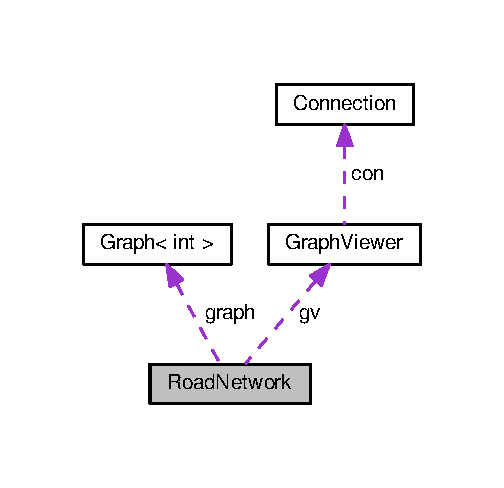
\includegraphics[width=242pt]{classRoadNetwork__coll__graph}
\end{center}
\end{figure}
\subsection*{Public Member Functions}
\begin{DoxyCompactItemize}
\item 
\hyperlink{classRoadNetwork_a635cd53a27194c18870f6afc1f9e54cf}{Road\+Network} ()
\item 
virtual \hyperlink{classRoadNetwork_a03a442c7c5c89bab9bb10632caefd2eb}{$\sim$\+Road\+Network} ()
\item 
void \hyperlink{classRoadNetwork_abf74962fc6a63d82efcd0073c48b0d35}{read\+O\+SM} ()
\item 
void \hyperlink{classRoadNetwork_a8b2c18eac996760101db4afc6c114b14}{write\+Edge\+File} ()
\item 
void \hyperlink{classRoadNetwork_a280633c5b00df3dfc59bc677fc12daa3}{convert\+To\+GV} ()
\item 
const \hyperlink{classGraph}{Graph}$<$ int $>$ \& \hyperlink{classRoadNetwork_a64106d7ec4e6b2953197b617fe0630bf}{get\+Graph} () const 
\item 
bool \hyperlink{classRoadNetwork_a60e0a20c8e393740c81fa47bc42bf9cd}{get\+Edge\+Blocked\+Status} (string name)
\item 
void \hyperlink{classRoadNetwork_a981b13a5dcab7fb5a1089d0a53fc788d}{set\+Edge\+Blocked} (string edge\+\_\+name, bool blocked)
\item 
double \hyperlink{classRoadNetwork_aa443cb868d60554dbec1b72c009c13ab}{get\+Weight\+Of\+Path} (vector$<$ \hyperlink{classVertex}{Vertex}$<$ int $>$ $\ast$ $>$ vec)
\item 
void \hyperlink{classRoadNetwork_ae48e55423eb4341d38634ecaa2c5f928}{print\+Path} (int node\+Start\+ID, int node\+Destination\+ID)
\item 
void \hyperlink{classRoadNetwork_af205756860697944d8f37490dd0b9e35}{print\+All\+Car\+Path} () const 
\item 
void \hyperlink{classRoadNetwork_ac4badf08e6ff3cfaff7e6e3a3f9efc3f}{print\+Car\+ID} () const 
\item 
bool \hyperlink{classRoadNetwork_a47cedd456d5f101e2759237f65bb0ff1}{remove\+Car} (int id)
\item 
void \hyperlink{classRoadNetwork_ac84b2b00026bff9f86b176eeea850c85}{write\+Cars\+File} ()
\item 
void \hyperlink{classRoadNetwork_aaac7323e85fb420874c33f43cf86c298}{highlight\+Node} (int id) const 
\item 
void \hyperlink{classRoadNetwork_ac25e6fa1448a8d04b7ca66fcf7a75a07}{highlight\+Edge} (int id) const 
\item 
void \hyperlink{classRoadNetwork_a0d4ef3d749cde1cdfb80f9c746d6bcae}{remove\+Highlight\+Node} (int id) const 
\item 
void \hyperlink{classRoadNetwork_a35109f4ee0222e27403887edfe11f98c}{remove\+Highlight\+Edge} (int id) const 
\item 
void \hyperlink{classRoadNetwork_abd95729335a21500f7865a30b22de321}{block\+Edge} (int id) const 
\item 
void \hyperlink{classRoadNetwork_ae995079ae1db8453fcfdf223ed5b4481}{remove\+Block\+Edge} (int id) const 
\item 
void \hyperlink{classRoadNetwork_ac1eaa1c584e4be1a720bbe975f3fdaf3}{update\+Map} () const 
\item 
void \hyperlink{classRoadNetwork_a53885e421d68d12e5e29222fc388e156}{close\+Map\+Window} () const 
\item 
void \hyperlink{classRoadNetwork_ad0d2c77f25ade353665e8ca11e1775fa}{update\+Info} ()
\end{DoxyCompactItemize}
\subsection*{Private Attributes}
\begin{DoxyCompactItemize}
\item 
\hyperlink{classGraph}{Graph}$<$ int $>$ \hyperlink{classRoadNetwork_aecef1ce1d95a05cccb98b345bae951ad}{graph}
\item 
\hyperlink{classGraphViewer}{Graph\+Viewer} $\ast$ \hyperlink{classRoadNetwork_a3512bc7d6e202925537873f3e769141c}{gv}
\end{DoxyCompactItemize}


\subsection{Detailed Description}
Classe que guarda todas as informacoes necessarias, que faz todos os calculos necessarios com essas informacoes e atualiza o graphviewer 

\subsection{Constructor \& Destructor Documentation}
\index{Road\+Network@{Road\+Network}!Road\+Network@{Road\+Network}}
\index{Road\+Network@{Road\+Network}!Road\+Network@{Road\+Network}}
\subsubsection[{\texorpdfstring{Road\+Network()}{RoadNetwork()}}]{\setlength{\rightskip}{0pt plus 5cm}Road\+Network\+::\+Road\+Network (
\begin{DoxyParamCaption}
{}
\end{DoxyParamCaption}
)}\hypertarget{classRoadNetwork_a635cd53a27194c18870f6afc1f9e54cf}{}\label{classRoadNetwork_a635cd53a27194c18870f6afc1f9e54cf}
Construtor \index{Road\+Network@{Road\+Network}!````~Road\+Network@{$\sim$\+Road\+Network}}
\index{````~Road\+Network@{$\sim$\+Road\+Network}!Road\+Network@{Road\+Network}}
\subsubsection[{\texorpdfstring{$\sim$\+Road\+Network()}{~RoadNetwork()}}]{\setlength{\rightskip}{0pt plus 5cm}Road\+Network\+::$\sim$\+Road\+Network (
\begin{DoxyParamCaption}
{}
\end{DoxyParamCaption}
)\hspace{0.3cm}{\ttfamily [virtual]}}\hypertarget{classRoadNetwork_a03a442c7c5c89bab9bb10632caefd2eb}{}\label{classRoadNetwork_a03a442c7c5c89bab9bb10632caefd2eb}
Destrutor 

\subsection{Member Function Documentation}
\index{Road\+Network@{Road\+Network}!block\+Edge@{block\+Edge}}
\index{block\+Edge@{block\+Edge}!Road\+Network@{Road\+Network}}
\subsubsection[{\texorpdfstring{block\+Edge(int id) const }{blockEdge(int id) const }}]{\setlength{\rightskip}{0pt plus 5cm}void Road\+Network\+::block\+Edge (
\begin{DoxyParamCaption}
\item[{int}]{id}
\end{DoxyParamCaption}
) const}\hypertarget{classRoadNetwork_abd95729335a21500f7865a30b22de321}{}\label{classRoadNetwork_abd95729335a21500f7865a30b22de321}
Atualiza a cor de uma edge para a preto (bloqueada) 
\begin{DoxyParams}{Parameters}
{\em id} & id da edge a atualizar \\
\hline
\end{DoxyParams}
\index{Road\+Network@{Road\+Network}!close\+Map\+Window@{close\+Map\+Window}}
\index{close\+Map\+Window@{close\+Map\+Window}!Road\+Network@{Road\+Network}}
\subsubsection[{\texorpdfstring{close\+Map\+Window() const }{closeMapWindow() const }}]{\setlength{\rightskip}{0pt plus 5cm}void Road\+Network\+::close\+Map\+Window (
\begin{DoxyParamCaption}
{}
\end{DoxyParamCaption}
) const}\hypertarget{classRoadNetwork_a53885e421d68d12e5e29222fc388e156}{}\label{classRoadNetwork_a53885e421d68d12e5e29222fc388e156}
Fecha a janela do graphviewer \index{Road\+Network@{Road\+Network}!convert\+To\+GV@{convert\+To\+GV}}
\index{convert\+To\+GV@{convert\+To\+GV}!Road\+Network@{Road\+Network}}
\subsubsection[{\texorpdfstring{convert\+To\+G\+V()}{convertToGV()}}]{\setlength{\rightskip}{0pt plus 5cm}void Road\+Network\+::convert\+To\+GV (
\begin{DoxyParamCaption}
{}
\end{DoxyParamCaption}
)}\hypertarget{classRoadNetwork_a280633c5b00df3dfc59bc677fc12daa3}{}\label{classRoadNetwork_a280633c5b00df3dfc59bc677fc12daa3}
Converte a informacao contida no grafo numa do tipo graphviewer \index{Road\+Network@{Road\+Network}!get\+Edge\+Blocked\+Status@{get\+Edge\+Blocked\+Status}}
\index{get\+Edge\+Blocked\+Status@{get\+Edge\+Blocked\+Status}!Road\+Network@{Road\+Network}}
\subsubsection[{\texorpdfstring{get\+Edge\+Blocked\+Status(string name)}{getEdgeBlockedStatus(string name)}}]{\setlength{\rightskip}{0pt plus 5cm}bool Road\+Network\+::get\+Edge\+Blocked\+Status (
\begin{DoxyParamCaption}
\item[{string}]{name}
\end{DoxyParamCaption}
)}\hypertarget{classRoadNetwork_a60e0a20c8e393740c81fa47bc42bf9cd}{}\label{classRoadNetwork_a60e0a20c8e393740c81fa47bc42bf9cd}
Indica se uma estrada se encontra bloqueada ou nao 
\begin{DoxyParams}{Parameters}
{\em name} & nome da estrada que se pretende verificar \\
\hline
\end{DoxyParams}
\begin{DoxyReturn}{Returns}
true se estiver bloqueada, false se nao 
\end{DoxyReturn}
\index{Road\+Network@{Road\+Network}!get\+Graph@{get\+Graph}}
\index{get\+Graph@{get\+Graph}!Road\+Network@{Road\+Network}}
\subsubsection[{\texorpdfstring{get\+Graph() const }{getGraph() const }}]{\setlength{\rightskip}{0pt plus 5cm}const {\bf Graph}$<$ int $>$ \& Road\+Network\+::get\+Graph (
\begin{DoxyParamCaption}
{}
\end{DoxyParamCaption}
) const}\hypertarget{classRoadNetwork_a64106d7ec4e6b2953197b617fe0630bf}{}\label{classRoadNetwork_a64106d7ec4e6b2953197b617fe0630bf}
Devolve o grafo \begin{DoxyReturn}{Returns}
grafo 
\end{DoxyReturn}
\index{Road\+Network@{Road\+Network}!get\+Weight\+Of\+Path@{get\+Weight\+Of\+Path}}
\index{get\+Weight\+Of\+Path@{get\+Weight\+Of\+Path}!Road\+Network@{Road\+Network}}
\subsubsection[{\texorpdfstring{get\+Weight\+Of\+Path(vector$<$ Vertex$<$ int $>$ $\ast$ $>$ vec)}{getWeightOfPath(vector< Vertex< int > * > vec)}}]{\setlength{\rightskip}{0pt plus 5cm}double Road\+Network\+::get\+Weight\+Of\+Path (
\begin{DoxyParamCaption}
\item[{vector$<$ {\bf Vertex}$<$ int $>$ $\ast$ $>$}]{vec}
\end{DoxyParamCaption}
)}\hypertarget{classRoadNetwork_aa443cb868d60554dbec1b72c009c13ab}{}\label{classRoadNetwork_aa443cb868d60554dbec1b72c009c13ab}
Devolve o peso total de um percurso 
\begin{DoxyParams}{Parameters}
{\em vec} & vetor com os vertices do percurso a calcular \\
\hline
\end{DoxyParams}
\begin{DoxyReturn}{Returns}
valor do peso do percurso 
\end{DoxyReturn}
\index{Road\+Network@{Road\+Network}!highlight\+Edge@{highlight\+Edge}}
\index{highlight\+Edge@{highlight\+Edge}!Road\+Network@{Road\+Network}}
\subsubsection[{\texorpdfstring{highlight\+Edge(int id) const }{highlightEdge(int id) const }}]{\setlength{\rightskip}{0pt plus 5cm}void Road\+Network\+::highlight\+Edge (
\begin{DoxyParamCaption}
\item[{int}]{id}
\end{DoxyParamCaption}
) const}\hypertarget{classRoadNetwork_ac25e6fa1448a8d04b7ca66fcf7a75a07}{}\label{classRoadNetwork_ac25e6fa1448a8d04b7ca66fcf7a75a07}
Atualiza a cor de uma edge no graphviewer para amarelo (percurso) 
\begin{DoxyParams}{Parameters}
{\em id} & id da edge a atualizar \\
\hline
\end{DoxyParams}
\index{Road\+Network@{Road\+Network}!highlight\+Node@{highlight\+Node}}
\index{highlight\+Node@{highlight\+Node}!Road\+Network@{Road\+Network}}
\subsubsection[{\texorpdfstring{highlight\+Node(int id) const }{highlightNode(int id) const }}]{\setlength{\rightskip}{0pt plus 5cm}void Road\+Network\+::highlight\+Node (
\begin{DoxyParamCaption}
\item[{int}]{id}
\end{DoxyParamCaption}
) const}\hypertarget{classRoadNetwork_aaac7323e85fb420874c33f43cf86c298}{}\label{classRoadNetwork_aaac7323e85fb420874c33f43cf86c298}
Atualiza a cor de um vertice no graphviewer para amarelo (percurso) 
\begin{DoxyParams}{Parameters}
{\em id} & id do vertice a atualizar \\
\hline
\end{DoxyParams}
\index{Road\+Network@{Road\+Network}!print\+All\+Car\+Path@{print\+All\+Car\+Path}}
\index{print\+All\+Car\+Path@{print\+All\+Car\+Path}!Road\+Network@{Road\+Network}}
\subsubsection[{\texorpdfstring{print\+All\+Car\+Path() const }{printAllCarPath() const }}]{\setlength{\rightskip}{0pt plus 5cm}void Road\+Network\+::print\+All\+Car\+Path (
\begin{DoxyParamCaption}
{}
\end{DoxyParamCaption}
) const}\hypertarget{classRoadNetwork_af205756860697944d8f37490dd0b9e35}{}\label{classRoadNetwork_af205756860697944d8f37490dd0b9e35}
Imprime o percurso completo de todos os carros \index{Road\+Network@{Road\+Network}!print\+Car\+ID@{print\+Car\+ID}}
\index{print\+Car\+ID@{print\+Car\+ID}!Road\+Network@{Road\+Network}}
\subsubsection[{\texorpdfstring{print\+Car\+I\+D() const }{printCarID() const }}]{\setlength{\rightskip}{0pt plus 5cm}void Road\+Network\+::print\+Car\+ID (
\begin{DoxyParamCaption}
{}
\end{DoxyParamCaption}
) const}\hypertarget{classRoadNetwork_ac4badf08e6ff3cfaff7e6e3a3f9efc3f}{}\label{classRoadNetwork_ac4badf08e6ff3cfaff7e6e3a3f9efc3f}
Imprime o inicio e o fim do percurso de todos os carros \index{Road\+Network@{Road\+Network}!print\+Path@{print\+Path}}
\index{print\+Path@{print\+Path}!Road\+Network@{Road\+Network}}
\subsubsection[{\texorpdfstring{print\+Path(int node\+Start\+I\+D, int node\+Destination\+I\+D)}{printPath(int nodeStartID, int nodeDestinationID)}}]{\setlength{\rightskip}{0pt plus 5cm}void Road\+Network\+::print\+Path (
\begin{DoxyParamCaption}
\item[{int}]{node\+Start\+ID, }
\item[{int}]{node\+Destination\+ID}
\end{DoxyParamCaption}
)}\hypertarget{classRoadNetwork_ae48e55423eb4341d38634ecaa2c5f928}{}\label{classRoadNetwork_ae48e55423eb4341d38634ecaa2c5f928}
Imprime a informacao relativa a um percurso, atualizando, tambem, o graphviewer com. Adiciona um novo carro ao programa cada vez que é executada. 
\begin{DoxyParams}{Parameters}
{\em node\+Start\+ID} & \\
\hline
{\em node\+Destination\+ID} & \\
\hline
\end{DoxyParams}
\index{Road\+Network@{Road\+Network}!read\+O\+SM@{read\+O\+SM}}
\index{read\+O\+SM@{read\+O\+SM}!Road\+Network@{Road\+Network}}
\subsubsection[{\texorpdfstring{read\+O\+S\+M()}{readOSM()}}]{\setlength{\rightskip}{0pt plus 5cm}void Road\+Network\+::read\+O\+SM (
\begin{DoxyParamCaption}
{}
\end{DoxyParamCaption}
)}\hypertarget{classRoadNetwork_abf74962fc6a63d82efcd0073c48b0d35}{}\label{classRoadNetwork_abf74962fc6a63d82efcd0073c48b0d35}
Le os ficheiros com informacao relativa aos vertices, as edges e aos carros e atualiza o grafo com essa informacao \index{Road\+Network@{Road\+Network}!remove\+Block\+Edge@{remove\+Block\+Edge}}
\index{remove\+Block\+Edge@{remove\+Block\+Edge}!Road\+Network@{Road\+Network}}
\subsubsection[{\texorpdfstring{remove\+Block\+Edge(int id) const }{removeBlockEdge(int id) const }}]{\setlength{\rightskip}{0pt plus 5cm}void Road\+Network\+::remove\+Block\+Edge (
\begin{DoxyParamCaption}
\item[{int}]{id}
\end{DoxyParamCaption}
) const}\hypertarget{classRoadNetwork_ae995079ae1db8453fcfdf223ed5b4481}{}\label{classRoadNetwork_ae995079ae1db8453fcfdf223ed5b4481}
Atualiza a cor de uma edge para a sua cor padrao 
\begin{DoxyParams}{Parameters}
{\em id} & id da edge a atualizar \\
\hline
\end{DoxyParams}
\index{Road\+Network@{Road\+Network}!remove\+Car@{remove\+Car}}
\index{remove\+Car@{remove\+Car}!Road\+Network@{Road\+Network}}
\subsubsection[{\texorpdfstring{remove\+Car(int id)}{removeCar(int id)}}]{\setlength{\rightskip}{0pt plus 5cm}bool Road\+Network\+::remove\+Car (
\begin{DoxyParamCaption}
\item[{int}]{id}
\end{DoxyParamCaption}
)}\hypertarget{classRoadNetwork_a47cedd456d5f101e2759237f65bb0ff1}{}\label{classRoadNetwork_a47cedd456d5f101e2759237f65bb0ff1}
Remove um carro do programa 
\begin{DoxyParams}{Parameters}
{\em id} & id do carro a remover \\
\hline
\end{DoxyParams}
\begin{DoxyReturn}{Returns}
true so foi possivel remover, falso se nao 
\end{DoxyReturn}
\index{Road\+Network@{Road\+Network}!remove\+Highlight\+Edge@{remove\+Highlight\+Edge}}
\index{remove\+Highlight\+Edge@{remove\+Highlight\+Edge}!Road\+Network@{Road\+Network}}
\subsubsection[{\texorpdfstring{remove\+Highlight\+Edge(int id) const }{removeHighlightEdge(int id) const }}]{\setlength{\rightskip}{0pt plus 5cm}void Road\+Network\+::remove\+Highlight\+Edge (
\begin{DoxyParamCaption}
\item[{int}]{id}
\end{DoxyParamCaption}
) const}\hypertarget{classRoadNetwork_a35109f4ee0222e27403887edfe11f98c}{}\label{classRoadNetwork_a35109f4ee0222e27403887edfe11f98c}
Atualiza a cor de uma edge para a sua cor padrao 
\begin{DoxyParams}{Parameters}
{\em id} & id da edge a atualizar \\
\hline
\end{DoxyParams}
\index{Road\+Network@{Road\+Network}!remove\+Highlight\+Node@{remove\+Highlight\+Node}}
\index{remove\+Highlight\+Node@{remove\+Highlight\+Node}!Road\+Network@{Road\+Network}}
\subsubsection[{\texorpdfstring{remove\+Highlight\+Node(int id) const }{removeHighlightNode(int id) const }}]{\setlength{\rightskip}{0pt plus 5cm}void Road\+Network\+::remove\+Highlight\+Node (
\begin{DoxyParamCaption}
\item[{int}]{id}
\end{DoxyParamCaption}
) const}\hypertarget{classRoadNetwork_a0d4ef3d749cde1cdfb80f9c746d6bcae}{}\label{classRoadNetwork_a0d4ef3d749cde1cdfb80f9c746d6bcae}
Atualiza a cor de um vertice para a sua cor padrao 
\begin{DoxyParams}{Parameters}
{\em id} & id do vertice a atualizar \\
\hline
\end{DoxyParams}
\index{Road\+Network@{Road\+Network}!set\+Edge\+Blocked@{set\+Edge\+Blocked}}
\index{set\+Edge\+Blocked@{set\+Edge\+Blocked}!Road\+Network@{Road\+Network}}
\subsubsection[{\texorpdfstring{set\+Edge\+Blocked(string edge\+\_\+name, bool blocked)}{setEdgeBlocked(string edge_name, bool blocked)}}]{\setlength{\rightskip}{0pt plus 5cm}void Road\+Network\+::set\+Edge\+Blocked (
\begin{DoxyParamCaption}
\item[{string}]{edge\+\_\+name, }
\item[{bool}]{blocked}
\end{DoxyParamCaption}
)}\hypertarget{classRoadNetwork_a981b13a5dcab7fb5a1089d0a53fc788d}{}\label{classRoadNetwork_a981b13a5dcab7fb5a1089d0a53fc788d}
Altera o estado de bloqueada, ou nao, de uma estrada 
\begin{DoxyParams}{Parameters}
{\em edge\+\_\+name} & nome da estrada que se pretende alterar \\
\hline
{\em blocked} & novo valor \\
\hline
\end{DoxyParams}
\index{Road\+Network@{Road\+Network}!update\+Info@{update\+Info}}
\index{update\+Info@{update\+Info}!Road\+Network@{Road\+Network}}
\subsubsection[{\texorpdfstring{update\+Info()}{updateInfo()}}]{\setlength{\rightskip}{0pt plus 5cm}void Road\+Network\+::update\+Info (
\begin{DoxyParamCaption}
{}
\end{DoxyParamCaption}
)}\hypertarget{classRoadNetwork_ad0d2c77f25ade353665e8ca11e1775fa}{}\label{classRoadNetwork_ad0d2c77f25ade353665e8ca11e1775fa}
Atualiza o conteudo do grafo \index{Road\+Network@{Road\+Network}!update\+Map@{update\+Map}}
\index{update\+Map@{update\+Map}!Road\+Network@{Road\+Network}}
\subsubsection[{\texorpdfstring{update\+Map() const }{updateMap() const }}]{\setlength{\rightskip}{0pt plus 5cm}void Road\+Network\+::update\+Map (
\begin{DoxyParamCaption}
{}
\end{DoxyParamCaption}
) const}\hypertarget{classRoadNetwork_ac1eaa1c584e4be1a720bbe975f3fdaf3}{}\label{classRoadNetwork_ac1eaa1c584e4be1a720bbe975f3fdaf3}
Atualiza a cor das edges tendo em conta o numero de carros que por ela circulam e se se encontra bloqueada ou nao \index{Road\+Network@{Road\+Network}!write\+Cars\+File@{write\+Cars\+File}}
\index{write\+Cars\+File@{write\+Cars\+File}!Road\+Network@{Road\+Network}}
\subsubsection[{\texorpdfstring{write\+Cars\+File()}{writeCarsFile()}}]{\setlength{\rightskip}{0pt plus 5cm}void Road\+Network\+::write\+Cars\+File (
\begin{DoxyParamCaption}
{}
\end{DoxyParamCaption}
)}\hypertarget{classRoadNetwork_ac84b2b00026bff9f86b176eeea850c85}{}\label{classRoadNetwork_ac84b2b00026bff9f86b176eeea850c85}
Escreve a informacao relativa a todos os carros no ficheiro \index{Road\+Network@{Road\+Network}!write\+Edge\+File@{write\+Edge\+File}}
\index{write\+Edge\+File@{write\+Edge\+File}!Road\+Network@{Road\+Network}}
\subsubsection[{\texorpdfstring{write\+Edge\+File()}{writeEdgeFile()}}]{\setlength{\rightskip}{0pt plus 5cm}void Road\+Network\+::write\+Edge\+File (
\begin{DoxyParamCaption}
{}
\end{DoxyParamCaption}
)}\hypertarget{classRoadNetwork_a8b2c18eac996760101db4afc6c114b14}{}\label{classRoadNetwork_a8b2c18eac996760101db4afc6c114b14}
Escreve a informacao das edges no ficheiro correspondente 

\subsection{Member Data Documentation}
\index{Road\+Network@{Road\+Network}!graph@{graph}}
\index{graph@{graph}!Road\+Network@{Road\+Network}}
\subsubsection[{\texorpdfstring{graph}{graph}}]{\setlength{\rightskip}{0pt plus 5cm}{\bf Graph}$<$int$>$ Road\+Network\+::graph\hspace{0.3cm}{\ttfamily [private]}}\hypertarget{classRoadNetwork_aecef1ce1d95a05cccb98b345bae951ad}{}\label{classRoadNetwork_aecef1ce1d95a05cccb98b345bae951ad}
Variavel que guarda o grafo \index{Road\+Network@{Road\+Network}!gv@{gv}}
\index{gv@{gv}!Road\+Network@{Road\+Network}}
\subsubsection[{\texorpdfstring{gv}{gv}}]{\setlength{\rightskip}{0pt plus 5cm}{\bf Graph\+Viewer}$\ast$ Road\+Network\+::gv\hspace{0.3cm}{\ttfamily [private]}}\hypertarget{classRoadNetwork_a3512bc7d6e202925537873f3e769141c}{}\label{classRoadNetwork_a3512bc7d6e202925537873f3e769141c}
Variavel que guarda o graphviewer 

The documentation for this class was generated from the following files\+:\begin{DoxyCompactItemize}
\item 
/home/amadeu/\+Desktop/\+Cal-\/2018/src/\hyperlink{RoadNetwork_8h}{Road\+Network.\+h}\item 
/home/amadeu/\+Desktop/\+Cal-\/2018/src/\hyperlink{RoadNetwork_8cpp}{Road\+Network.\+cpp}\end{DoxyCompactItemize}

\hypertarget{classVertex}{}\section{Vertex$<$ T $>$ Class Template Reference}
\label{classVertex}\index{Vertex$<$ T $>$@{Vertex$<$ T $>$}}


{\ttfamily \#include $<$Graph.\+h$>$}

\subsection*{Public Member Functions}
\begin{DoxyCompactItemize}
\item 
\hyperlink{classVertex_a379ed46a1fc16ae01d69cbd071d5d708}{Vertex} (T in, string \hyperlink{classVertex_a1990577b54c37df981c81eac40c4af71}{name}, double lon, double lat)
\item 
bool \hyperlink{classVertex_a769abfb2961e1f1e66e3b9be6b3f4617}{operator$<$} (\hyperlink{classVertex}{Vertex}$<$ T $>$ \&vertex) const 
\item 
T \hyperlink{classVertex_a5880b4b252ae6818819c2f9645784b59}{get\+Info} () const 
\item 
vector$<$ \hyperlink{classEdge}{Edge}$<$ T $>$ $\ast$ $>$ \hyperlink{classVertex_a39f23de20a5de4f6362a20a2d8d14cf0}{get\+Adj} () const 
\item 
void \hyperlink{classVertex_a7961dc8c855dca6e90fd759f54d1ff18}{add\+Edge} (\hyperlink{classVertex}{Vertex}$<$ T $>$ $\ast$d, double w, bool tw, string n, T id, bool block)
\item 
bool \hyperlink{classVertex_ab2b5b43fb1709a901b78718436763a84}{remove\+Edge\+To} (\hyperlink{classVertex}{Vertex}$<$ T $>$ $\ast$d)
\item 
string \hyperlink{classVertex_a878c08e3eca2b53b173fa8c1fa77227d}{get\+Name} () const 
\item 
void \hyperlink{classVertex_aee1d15f2efc9c7baecff72265beb1acf}{set\+Name} (string \hyperlink{classVertex_a1990577b54c37df981c81eac40c4af71}{name})
\item 
double \hyperlink{classVertex_aa88dbd3c9af86b1fd567a43c0da69017}{get\+Longitude} () const 
\item 
double \hyperlink{classVertex_afbf6474fe17f4fd509bda1026fd81385}{get\+Latitude} () const 
\item 
double \hyperlink{classVertex_a5c5b34281128297a4824b1c377d2b788}{get\+Dist} () const 
\item 
\hyperlink{classVertex}{Vertex}$<$ T $>$ $\ast$ \hyperlink{classVertex_ae0b57c953450db1679e5f5994e1ba738}{get\+Path} () const 
\item 
\hyperlink{classEdge}{Edge}$<$ T $>$ $\ast$ \hyperlink{classVertex_a695e48fb6e5ad425348b47a88dafe065}{get\+Caminho} () const 
\end{DoxyCompactItemize}
\subsection*{Private Attributes}
\begin{DoxyCompactItemize}
\item 
T \hyperlink{classVertex_a415d7811eef6cdd992f0dca1f35a49cd}{info}
\item 
vector$<$ \hyperlink{classEdge}{Edge}$<$ T $>$ $\ast$ $>$ \hyperlink{classVertex_a3a5e3cdc85b3d338a5661cb5b55de729}{adj}
\item 
bool \hyperlink{classVertex_a187a2fe4ff50261cf3c15b8cda7dfc56}{visited}
\item 
int \hyperlink{classVertex_ab29ac1b694fc673ba26cfc6d3e9bda13}{indegree}
\item 
string \hyperlink{classVertex_a1990577b54c37df981c81eac40c4af71}{name}
\item 
double \hyperlink{classVertex_a960be3c1167e82abe7fcb81178674e5e}{latitude}
\item 
double \hyperlink{classVertex_a830e29c233af0899c087d9873864c477}{longitude}
\item 
double \hyperlink{classVertex_a08a2b813e77f97aa8b6c1d252e5417f7}{dist} = 0
\item 
\hyperlink{classVertex}{Vertex}$<$ T $>$ $\ast$ \hyperlink{classVertex_ab968bdd80f912a6f21f30e479bf735ce}{path} = N\+U\+LL
\item 
\hyperlink{classEdge}{Edge}$<$ T $>$ $\ast$ \hyperlink{classVertex_adb879f0355fa2d27be89fe9286fdfd4a}{caminho} = N\+U\+LL
\item 
int \hyperlink{classVertex_a721ab622207a73c5fae7b9abad6c07cc}{queue\+Index} = 0
\end{DoxyCompactItemize}
\subsection*{Friends}
\begin{DoxyCompactItemize}
\item 
class \hyperlink{classVertex_ae53e0b4fec14b9f1eaa8a4f8cd426e9e}{Mutable\+Priority\+Queue$<$ Vertex$<$ T $>$ $>$}
\item 
class \hyperlink{classVertex_aefa9b76cd57411c5354e5620dc2d84dd}{Graph$<$ T $>$}
\end{DoxyCompactItemize}


\subsection{Detailed Description}
\subsubsection*{template$<$class T$>$\\*
class Vertex$<$ T $>$}

class que representa um vertice do grafo 

\subsection{Constructor \& Destructor Documentation}
\index{Vertex@{Vertex}!Vertex@{Vertex}}
\index{Vertex@{Vertex}!Vertex@{Vertex}}
\subsubsection[{\texorpdfstring{Vertex(\+T in, string name, double lon, double lat)}{Vertex(T in, string name, double lon, double lat)}}]{\setlength{\rightskip}{0pt plus 5cm}template$<$class T $>$ {\bf Vertex}$<$ T $>$\+::{\bf Vertex} (
\begin{DoxyParamCaption}
\item[{T}]{in, }
\item[{string}]{name, }
\item[{double}]{lon, }
\item[{double}]{lat}
\end{DoxyParamCaption}
)}\hypertarget{classVertex_a379ed46a1fc16ae01d69cbd071d5d708}{}\label{classVertex_a379ed46a1fc16ae01d69cbd071d5d708}
construtor da class \hyperlink{classVertex}{Vertex} 
\begin{DoxyParams}{Parameters}
{\em in} & informa��o do vertice \\
\hline
{\em name} & nome do vertice \\
\hline
{\em lon} & londitude do vertice \\
\hline
{\em lat} & latitude do vertice \\
\hline
\end{DoxyParams}


\subsection{Member Function Documentation}
\index{Vertex@{Vertex}!add\+Edge@{add\+Edge}}
\index{add\+Edge@{add\+Edge}!Vertex@{Vertex}}
\subsubsection[{\texorpdfstring{add\+Edge(\+Vertex$<$ T $>$ $\ast$d, double w, bool tw, string n, T id, bool block)}{addEdge(Vertex< T > *d, double w, bool tw, string n, T id, bool block)}}]{\setlength{\rightskip}{0pt plus 5cm}template$<$class T $>$ void {\bf Vertex}$<$ T $>$\+::add\+Edge (
\begin{DoxyParamCaption}
\item[{{\bf Vertex}$<$ T $>$ $\ast$}]{d, }
\item[{double}]{w, }
\item[{bool}]{tw, }
\item[{string}]{n, }
\item[{T}]{id, }
\item[{bool}]{block}
\end{DoxyParamCaption}
)}\hypertarget{classVertex_a7961dc8c855dca6e90fd759f54d1ff18}{}\label{classVertex_a7961dc8c855dca6e90fd759f54d1ff18}
Adiciona uma aresta nova ao vector de arestas 
\begin{DoxyParams}{Parameters}
{\em d} & destino da aresta \\
\hline
{\em w} & peso da aresta \\
\hline
{\em tw} & se � de 2 sentidos a estrada \\
\hline
{\em n} & nome da aresta \\
\hline
{\em id} & id da aresta \\
\hline
{\em block} & se esta bloqueada \\
\hline
\end{DoxyParams}
\index{Vertex@{Vertex}!get\+Adj@{get\+Adj}}
\index{get\+Adj@{get\+Adj}!Vertex@{Vertex}}
\subsubsection[{\texorpdfstring{get\+Adj() const }{getAdj() const }}]{\setlength{\rightskip}{0pt plus 5cm}template$<$class T $>$ vector$<$ {\bf Edge}$<$ T $>$ $\ast$ $>$ {\bf Vertex}$<$ T $>$\+::get\+Adj (
\begin{DoxyParamCaption}
{}
\end{DoxyParamCaption}
) const}\hypertarget{classVertex_a39f23de20a5de4f6362a20a2d8d14cf0}{}\label{classVertex_a39f23de20a5de4f6362a20a2d8d14cf0}
\begin{DoxyReturn}{Returns}
returna o vector de arestas do vertice 
\end{DoxyReturn}
\index{Vertex@{Vertex}!get\+Caminho@{get\+Caminho}}
\index{get\+Caminho@{get\+Caminho}!Vertex@{Vertex}}
\subsubsection[{\texorpdfstring{get\+Caminho() const }{getCaminho() const }}]{\setlength{\rightskip}{0pt plus 5cm}template$<$class T $>$ {\bf Edge}$<$ T $>$ $\ast$ {\bf Vertex}$<$ T $>$\+::get\+Caminho (
\begin{DoxyParamCaption}
{}
\end{DoxyParamCaption}
) const}\hypertarget{classVertex_a695e48fb6e5ad425348b47a88dafe065}{}\label{classVertex_a695e48fb6e5ad425348b47a88dafe065}
\begin{DoxyReturn}{Returns}
returna a proxima aresta do caminho 
\end{DoxyReturn}
\index{Vertex@{Vertex}!get\+Dist@{get\+Dist}}
\index{get\+Dist@{get\+Dist}!Vertex@{Vertex}}
\subsubsection[{\texorpdfstring{get\+Dist() const }{getDist() const }}]{\setlength{\rightskip}{0pt plus 5cm}template$<$class T $>$ double {\bf Vertex}$<$ T $>$\+::get\+Dist (
\begin{DoxyParamCaption}
{}
\end{DoxyParamCaption}
) const}\hypertarget{classVertex_a5c5b34281128297a4824b1c377d2b788}{}\label{classVertex_a5c5b34281128297a4824b1c377d2b788}
\begin{DoxyReturn}{Returns}
returna a distancia do vertice 
\end{DoxyReturn}
\index{Vertex@{Vertex}!get\+Info@{get\+Info}}
\index{get\+Info@{get\+Info}!Vertex@{Vertex}}
\subsubsection[{\texorpdfstring{get\+Info() const }{getInfo() const }}]{\setlength{\rightskip}{0pt plus 5cm}template$<$class T $>$ T {\bf Vertex}$<$ T $>$\+::get\+Info (
\begin{DoxyParamCaption}
{}
\end{DoxyParamCaption}
) const}\hypertarget{classVertex_a5880b4b252ae6818819c2f9645784b59}{}\label{classVertex_a5880b4b252ae6818819c2f9645784b59}
\begin{DoxyReturn}{Returns}
returna a informa��o do vertice 
\end{DoxyReturn}
\index{Vertex@{Vertex}!get\+Latitude@{get\+Latitude}}
\index{get\+Latitude@{get\+Latitude}!Vertex@{Vertex}}
\subsubsection[{\texorpdfstring{get\+Latitude() const }{getLatitude() const }}]{\setlength{\rightskip}{0pt plus 5cm}template$<$class T $>$ double {\bf Vertex}$<$ T $>$\+::get\+Latitude (
\begin{DoxyParamCaption}
{}
\end{DoxyParamCaption}
) const}\hypertarget{classVertex_afbf6474fe17f4fd509bda1026fd81385}{}\label{classVertex_afbf6474fe17f4fd509bda1026fd81385}
\begin{DoxyReturn}{Returns}
returna a latitude do vertice 
\end{DoxyReturn}
\index{Vertex@{Vertex}!get\+Longitude@{get\+Longitude}}
\index{get\+Longitude@{get\+Longitude}!Vertex@{Vertex}}
\subsubsection[{\texorpdfstring{get\+Longitude() const }{getLongitude() const }}]{\setlength{\rightskip}{0pt plus 5cm}template$<$class T $>$ double {\bf Vertex}$<$ T $>$\+::get\+Longitude (
\begin{DoxyParamCaption}
{}
\end{DoxyParamCaption}
) const}\hypertarget{classVertex_aa88dbd3c9af86b1fd567a43c0da69017}{}\label{classVertex_aa88dbd3c9af86b1fd567a43c0da69017}
\begin{DoxyReturn}{Returns}
returna a longitude do vertice 
\end{DoxyReturn}
\index{Vertex@{Vertex}!get\+Name@{get\+Name}}
\index{get\+Name@{get\+Name}!Vertex@{Vertex}}
\subsubsection[{\texorpdfstring{get\+Name() const }{getName() const }}]{\setlength{\rightskip}{0pt plus 5cm}template$<$class T $>$ string {\bf Vertex}$<$ T $>$\+::get\+Name (
\begin{DoxyParamCaption}
{}
\end{DoxyParamCaption}
) const}\hypertarget{classVertex_a878c08e3eca2b53b173fa8c1fa77227d}{}\label{classVertex_a878c08e3eca2b53b173fa8c1fa77227d}
\begin{DoxyReturn}{Returns}
returna o nome do vertice 
\end{DoxyReturn}
\index{Vertex@{Vertex}!get\+Path@{get\+Path}}
\index{get\+Path@{get\+Path}!Vertex@{Vertex}}
\subsubsection[{\texorpdfstring{get\+Path() const }{getPath() const }}]{\setlength{\rightskip}{0pt plus 5cm}template$<$class T $>$ {\bf Vertex}$<$ T $>$ $\ast$ {\bf Vertex}$<$ T $>$\+::get\+Path (
\begin{DoxyParamCaption}
{}
\end{DoxyParamCaption}
) const}\hypertarget{classVertex_ae0b57c953450db1679e5f5994e1ba738}{}\label{classVertex_ae0b57c953450db1679e5f5994e1ba738}
\begin{DoxyReturn}{Returns}
returna o proximo vertice do caminho 
\end{DoxyReturn}
\index{Vertex@{Vertex}!operator$<$@{operator$<$}}
\index{operator$<$@{operator$<$}!Vertex@{Vertex}}
\subsubsection[{\texorpdfstring{operator$<$(\+Vertex$<$ T $>$ \&vertex) const }{operator<(Vertex< T > &vertex) const }}]{\setlength{\rightskip}{0pt plus 5cm}template$<$class T $>$ bool {\bf Vertex}$<$ T $>$\+::operator$<$ (
\begin{DoxyParamCaption}
\item[{{\bf Vertex}$<$ T $>$ \&}]{vertex}
\end{DoxyParamCaption}
) const}\hypertarget{classVertex_a769abfb2961e1f1e66e3b9be6b3f4617}{}\label{classVertex_a769abfb2961e1f1e66e3b9be6b3f4617}
Overload do operador $<$ para a class mutablepriorityqueue 
\begin{DoxyParams}{Parameters}
{\em vertex} & vertice que quero comparar \\
\hline
\end{DoxyParams}
\begin{DoxyReturn}{Returns}
boolean true de dist$<$dist ou false caso contrario 
\end{DoxyReturn}
\index{Vertex@{Vertex}!remove\+Edge\+To@{remove\+Edge\+To}}
\index{remove\+Edge\+To@{remove\+Edge\+To}!Vertex@{Vertex}}
\subsubsection[{\texorpdfstring{remove\+Edge\+To(\+Vertex$<$ T $>$ $\ast$d)}{removeEdgeTo(Vertex< T > *d)}}]{\setlength{\rightskip}{0pt plus 5cm}template$<$class T $>$ bool {\bf Vertex}$<$ T $>$\+::remove\+Edge\+To (
\begin{DoxyParamCaption}
\item[{{\bf Vertex}$<$ T $>$ $\ast$}]{d}
\end{DoxyParamCaption}
)}\hypertarget{classVertex_ab2b5b43fb1709a901b78718436763a84}{}\label{classVertex_ab2b5b43fb1709a901b78718436763a84}
Retira uma aresta do vector de arestas 
\begin{DoxyParams}{Parameters}
{\em d} & destino da aresta a retirar \\
\hline
\end{DoxyParams}
\begin{DoxyReturn}{Returns}
returna true se existe ou false caso contrario 
\end{DoxyReturn}
\index{Vertex@{Vertex}!set\+Name@{set\+Name}}
\index{set\+Name@{set\+Name}!Vertex@{Vertex}}
\subsubsection[{\texorpdfstring{set\+Name(string name)}{setName(string name)}}]{\setlength{\rightskip}{0pt plus 5cm}template$<$class T $>$ void {\bf Vertex}$<$ T $>$\+::set\+Name (
\begin{DoxyParamCaption}
\item[{string}]{name}
\end{DoxyParamCaption}
)}\hypertarget{classVertex_aee1d15f2efc9c7baecff72265beb1acf}{}\label{classVertex_aee1d15f2efc9c7baecff72265beb1acf}
define o nome da aresta 
\begin{DoxyParams}{Parameters}
{\em name} & nome que quero atribuir a aresta \\
\hline
\end{DoxyParams}


\subsection{Friends And Related Function Documentation}
\index{Vertex@{Vertex}!Graph$<$ T $>$@{Graph$<$ T $>$}}
\index{Graph$<$ T $>$@{Graph$<$ T $>$}!Vertex@{Vertex}}
\subsubsection[{\texorpdfstring{Graph$<$ T $>$}{Graph< T >}}]{\setlength{\rightskip}{0pt plus 5cm}template$<$class T$>$ friend class {\bf Graph}$<$ T $>$\hspace{0.3cm}{\ttfamily [friend]}}\hypertarget{classVertex_aefa9b76cd57411c5354e5620dc2d84dd}{}\label{classVertex_aefa9b76cd57411c5354e5620dc2d84dd}
\index{Vertex@{Vertex}!Mutable\+Priority\+Queue$<$ Vertex$<$ T $>$ $>$@{Mutable\+Priority\+Queue$<$ Vertex$<$ T $>$ $>$}}
\index{Mutable\+Priority\+Queue$<$ Vertex$<$ T $>$ $>$@{Mutable\+Priority\+Queue$<$ Vertex$<$ T $>$ $>$}!Vertex@{Vertex}}
\subsubsection[{\texorpdfstring{Mutable\+Priority\+Queue$<$ Vertex$<$ T $>$ $>$}{MutablePriorityQueue< Vertex< T > >}}]{\setlength{\rightskip}{0pt plus 5cm}template$<$class T$>$ friend class {\bf Mutable\+Priority\+Queue}$<$ {\bf Vertex}$<$ T $>$ $>$\hspace{0.3cm}{\ttfamily [friend]}}\hypertarget{classVertex_ae53e0b4fec14b9f1eaa8a4f8cd426e9e}{}\label{classVertex_ae53e0b4fec14b9f1eaa8a4f8cd426e9e}


\subsection{Member Data Documentation}
\index{Vertex@{Vertex}!adj@{adj}}
\index{adj@{adj}!Vertex@{Vertex}}
\subsubsection[{\texorpdfstring{adj}{adj}}]{\setlength{\rightskip}{0pt plus 5cm}template$<$class T$>$ vector$<${\bf Edge}$<$T$>$$\ast$$>$ {\bf Vertex}$<$ T $>$\+::adj\hspace{0.3cm}{\ttfamily [private]}}\hypertarget{classVertex_a3a5e3cdc85b3d338a5661cb5b55de729}{}\label{classVertex_a3a5e3cdc85b3d338a5661cb5b55de729}
vetor de arestas do vertice \index{Vertex@{Vertex}!caminho@{caminho}}
\index{caminho@{caminho}!Vertex@{Vertex}}
\subsubsection[{\texorpdfstring{caminho}{caminho}}]{\setlength{\rightskip}{0pt plus 5cm}template$<$class T$>$ {\bf Edge}$<$T$>$$\ast$ {\bf Vertex}$<$ T $>$\+::caminho = N\+U\+LL\hspace{0.3cm}{\ttfamily [private]}}\hypertarget{classVertex_adb879f0355fa2d27be89fe9286fdfd4a}{}\label{classVertex_adb879f0355fa2d27be89fe9286fdfd4a}
caminho para a procima aresta \index{Vertex@{Vertex}!dist@{dist}}
\index{dist@{dist}!Vertex@{Vertex}}
\subsubsection[{\texorpdfstring{dist}{dist}}]{\setlength{\rightskip}{0pt plus 5cm}template$<$class T$>$ double {\bf Vertex}$<$ T $>$\+::dist = 0\hspace{0.3cm}{\ttfamily [private]}}\hypertarget{classVertex_a08a2b813e77f97aa8b6c1d252e5417f7}{}\label{classVertex_a08a2b813e77f97aa8b6c1d252e5417f7}
distancia do vertice \index{Vertex@{Vertex}!indegree@{indegree}}
\index{indegree@{indegree}!Vertex@{Vertex}}
\subsubsection[{\texorpdfstring{indegree}{indegree}}]{\setlength{\rightskip}{0pt plus 5cm}template$<$class T$>$ int {\bf Vertex}$<$ T $>$\+::indegree\hspace{0.3cm}{\ttfamily [private]}}\hypertarget{classVertex_ab29ac1b694fc673ba26cfc6d3e9bda13}{}\label{classVertex_ab29ac1b694fc673ba26cfc6d3e9bda13}
indegree do vertice para a ordena��o topologica \index{Vertex@{Vertex}!info@{info}}
\index{info@{info}!Vertex@{Vertex}}
\subsubsection[{\texorpdfstring{info}{info}}]{\setlength{\rightskip}{0pt plus 5cm}template$<$class T$>$ T {\bf Vertex}$<$ T $>$\+::info\hspace{0.3cm}{\ttfamily [private]}}\hypertarget{classVertex_a415d7811eef6cdd992f0dca1f35a49cd}{}\label{classVertex_a415d7811eef6cdd992f0dca1f35a49cd}
informa��o do vertice \index{Vertex@{Vertex}!latitude@{latitude}}
\index{latitude@{latitude}!Vertex@{Vertex}}
\subsubsection[{\texorpdfstring{latitude}{latitude}}]{\setlength{\rightskip}{0pt plus 5cm}template$<$class T$>$ double {\bf Vertex}$<$ T $>$\+::latitude\hspace{0.3cm}{\ttfamily [private]}}\hypertarget{classVertex_a960be3c1167e82abe7fcb81178674e5e}{}\label{classVertex_a960be3c1167e82abe7fcb81178674e5e}
latitude do vertice \index{Vertex@{Vertex}!longitude@{longitude}}
\index{longitude@{longitude}!Vertex@{Vertex}}
\subsubsection[{\texorpdfstring{longitude}{longitude}}]{\setlength{\rightskip}{0pt plus 5cm}template$<$class T$>$ double {\bf Vertex}$<$ T $>$\+::longitude\hspace{0.3cm}{\ttfamily [private]}}\hypertarget{classVertex_a830e29c233af0899c087d9873864c477}{}\label{classVertex_a830e29c233af0899c087d9873864c477}
longitude do vertice \index{Vertex@{Vertex}!name@{name}}
\index{name@{name}!Vertex@{Vertex}}
\subsubsection[{\texorpdfstring{name}{name}}]{\setlength{\rightskip}{0pt plus 5cm}template$<$class T$>$ string {\bf Vertex}$<$ T $>$\+::name\hspace{0.3cm}{\ttfamily [private]}}\hypertarget{classVertex_a1990577b54c37df981c81eac40c4af71}{}\label{classVertex_a1990577b54c37df981c81eac40c4af71}
nome do vertice \index{Vertex@{Vertex}!path@{path}}
\index{path@{path}!Vertex@{Vertex}}
\subsubsection[{\texorpdfstring{path}{path}}]{\setlength{\rightskip}{0pt plus 5cm}template$<$class T$>$ {\bf Vertex}$<$T$>$$\ast$ {\bf Vertex}$<$ T $>$\+::path = N\+U\+LL\hspace{0.3cm}{\ttfamily [private]}}\hypertarget{classVertex_ab968bdd80f912a6f21f30e479bf735ce}{}\label{classVertex_ab968bdd80f912a6f21f30e479bf735ce}
caminho para o proximo vertice \index{Vertex@{Vertex}!queue\+Index@{queue\+Index}}
\index{queue\+Index@{queue\+Index}!Vertex@{Vertex}}
\subsubsection[{\texorpdfstring{queue\+Index}{queueIndex}}]{\setlength{\rightskip}{0pt plus 5cm}template$<$class T$>$ int {\bf Vertex}$<$ T $>$\+::queue\+Index = 0\hspace{0.3cm}{\ttfamily [private]}}\hypertarget{classVertex_a721ab622207a73c5fae7b9abad6c07cc}{}\label{classVertex_a721ab622207a73c5fae7b9abad6c07cc}
index para a mutablepriorityqueu \index{Vertex@{Vertex}!visited@{visited}}
\index{visited@{visited}!Vertex@{Vertex}}
\subsubsection[{\texorpdfstring{visited}{visited}}]{\setlength{\rightskip}{0pt plus 5cm}template$<$class T$>$ bool {\bf Vertex}$<$ T $>$\+::visited\hspace{0.3cm}{\ttfamily [private]}}\hypertarget{classVertex_a187a2fe4ff50261cf3c15b8cda7dfc56}{}\label{classVertex_a187a2fe4ff50261cf3c15b8cda7dfc56}
guarda o estado caso tenha o vertice tenha sido visitado 

The documentation for this class was generated from the following file\+:\begin{DoxyCompactItemize}
\item 
/home/amadeu/\+Desktop/\+Cal-\/2018/src/\hyperlink{Graph_8h}{Graph.\+h}\end{DoxyCompactItemize}

\hypertarget{structvertex__greater__than}{}\section{vertex\+\_\+greater\+\_\+than$<$ T $>$ Struct Template Reference}
\label{structvertex__greater__than}\index{vertex\+\_\+greater\+\_\+than$<$ T $>$@{vertex\+\_\+greater\+\_\+than$<$ T $>$}}


{\ttfamily \#include $<$Graph.\+h$>$}

\subsection*{Public Member Functions}
\begin{DoxyCompactItemize}
\item 
bool \hyperlink{structvertex__greater__than_af58940d572829488c2915ca53663631e}{operator()} (\hyperlink{classVertex}{Vertex}$<$ T $>$ $\ast$a, \hyperlink{classVertex}{Vertex}$<$ T $>$ $\ast$b) const 
\end{DoxyCompactItemize}


\subsection{Member Function Documentation}
\index{vertex\+\_\+greater\+\_\+than@{vertex\+\_\+greater\+\_\+than}!operator()@{operator()}}
\index{operator()@{operator()}!vertex\+\_\+greater\+\_\+than@{vertex\+\_\+greater\+\_\+than}}
\subsubsection[{\texorpdfstring{operator()(\+Vertex$<$ T $>$ $\ast$a, Vertex$<$ T $>$ $\ast$b) const }{operator()(Vertex< T > *a, Vertex< T > *b) const }}]{\setlength{\rightskip}{0pt plus 5cm}template$<$class T $>$ bool {\bf vertex\+\_\+greater\+\_\+than}$<$ T $>$\+::operator() (
\begin{DoxyParamCaption}
\item[{{\bf Vertex}$<$ T $>$ $\ast$}]{a, }
\item[{{\bf Vertex}$<$ T $>$ $\ast$}]{b}
\end{DoxyParamCaption}
) const\hspace{0.3cm}{\ttfamily [inline]}}\hypertarget{structvertex__greater__than_af58940d572829488c2915ca53663631e}{}\label{structvertex__greater__than_af58940d572829488c2915ca53663631e}


The documentation for this struct was generated from the following file\+:\begin{DoxyCompactItemize}
\item 
/home/amadeu/\+Desktop/\+Cal-\/2018/src/\hyperlink{Graph_8h}{Graph.\+h}\end{DoxyCompactItemize}

\chapter{File Documentation}
\hypertarget{connection_8cpp}{}\section{/\+Users/amadeuppereira/\+F\+E\+U\+P/2ano/\+Cal-\/2018/src/connection.cpp File Reference}
\label{connection_8cpp}\index{/\+Users/amadeuppereira/\+F\+E\+U\+P/2ano/\+Cal-\/2018/src/connection.\+cpp@{/\+Users/amadeuppereira/\+F\+E\+U\+P/2ano/\+Cal-\/2018/src/connection.\+cpp}}
{\ttfamily \#include \char`\"{}connection.\+h\char`\"{}}\newline
\subsection*{Macros}
\begin{DoxyCompactItemize}
\item 
\#define \mbox{\hyperlink{connection_8cpp_a258bb72419ef143530a2f8f55e7d57af}{N\+O\+\_\+\+E\+R\+R\+OR}}~0
\end{DoxyCompactItemize}
\subsection*{Functions}
\begin{DoxyCompactItemize}
\item 
void \mbox{\hyperlink{connection_8cpp_ac8b3411018d0e5416c08938b796177ab}{myerror}} (string msg)
\end{DoxyCompactItemize}


\subsection{Macro Definition Documentation}
\mbox{\Hypertarget{connection_8cpp_a258bb72419ef143530a2f8f55e7d57af}\label{connection_8cpp_a258bb72419ef143530a2f8f55e7d57af}} 
\index{connection.\+cpp@{connection.\+cpp}!N\+O\+\_\+\+E\+R\+R\+OR@{N\+O\+\_\+\+E\+R\+R\+OR}}
\index{N\+O\+\_\+\+E\+R\+R\+OR@{N\+O\+\_\+\+E\+R\+R\+OR}!connection.\+cpp@{connection.\+cpp}}
\subsubsection{\texorpdfstring{N\+O\+\_\+\+E\+R\+R\+OR}{NO\_ERROR}}
{\footnotesize\ttfamily \#define N\+O\+\_\+\+E\+R\+R\+OR~0}



\subsection{Function Documentation}
\mbox{\Hypertarget{connection_8cpp_ac8b3411018d0e5416c08938b796177ab}\label{connection_8cpp_ac8b3411018d0e5416c08938b796177ab}} 
\index{connection.\+cpp@{connection.\+cpp}!myerror@{myerror}}
\index{myerror@{myerror}!connection.\+cpp@{connection.\+cpp}}
\subsubsection{\texorpdfstring{myerror()}{myerror()}}
{\footnotesize\ttfamily void myerror (\begin{DoxyParamCaption}\item[{string}]{msg }\end{DoxyParamCaption})}


\hypertarget{connection_8h}{}\section{/\+Users/amadeuppereira/\+F\+E\+U\+P/2ano/\+Cal-\/2018/src/connection.h File Reference}
\label{connection_8h}\index{/\+Users/amadeuppereira/\+F\+E\+U\+P/2ano/\+Cal-\/2018/src/connection.\+h@{/\+Users/amadeuppereira/\+F\+E\+U\+P/2ano/\+Cal-\/2018/src/connection.\+h}}
{\ttfamily \#include $<$cstdio$>$}\newline
{\ttfamily \#include $<$cstdlib$>$}\newline
{\ttfamily \#include $<$cstring$>$}\newline
{\ttfamily \#include $<$winsock2.\+h$>$}\newline
{\ttfamily \#include $<$string$>$}\newline
{\ttfamily \#include $<$iostream$>$}\newline
\subsection*{Classes}
\begin{DoxyCompactItemize}
\item 
class \mbox{\hyperlink{class_connection}{Connection}}
\end{DoxyCompactItemize}

\hypertarget{edgetype_8h}{}\section{/home/amadeu/\+Desktop/\+Cal-\/2018/src/edgetype.h File Reference}
\label{edgetype_8h}\index{/home/amadeu/\+Desktop/\+Cal-\/2018/src/edgetype.\+h@{/home/amadeu/\+Desktop/\+Cal-\/2018/src/edgetype.\+h}}
This graph shows which files directly or indirectly include this file\+:\nopagebreak
\begin{figure}[H]
\begin{center}
\leavevmode
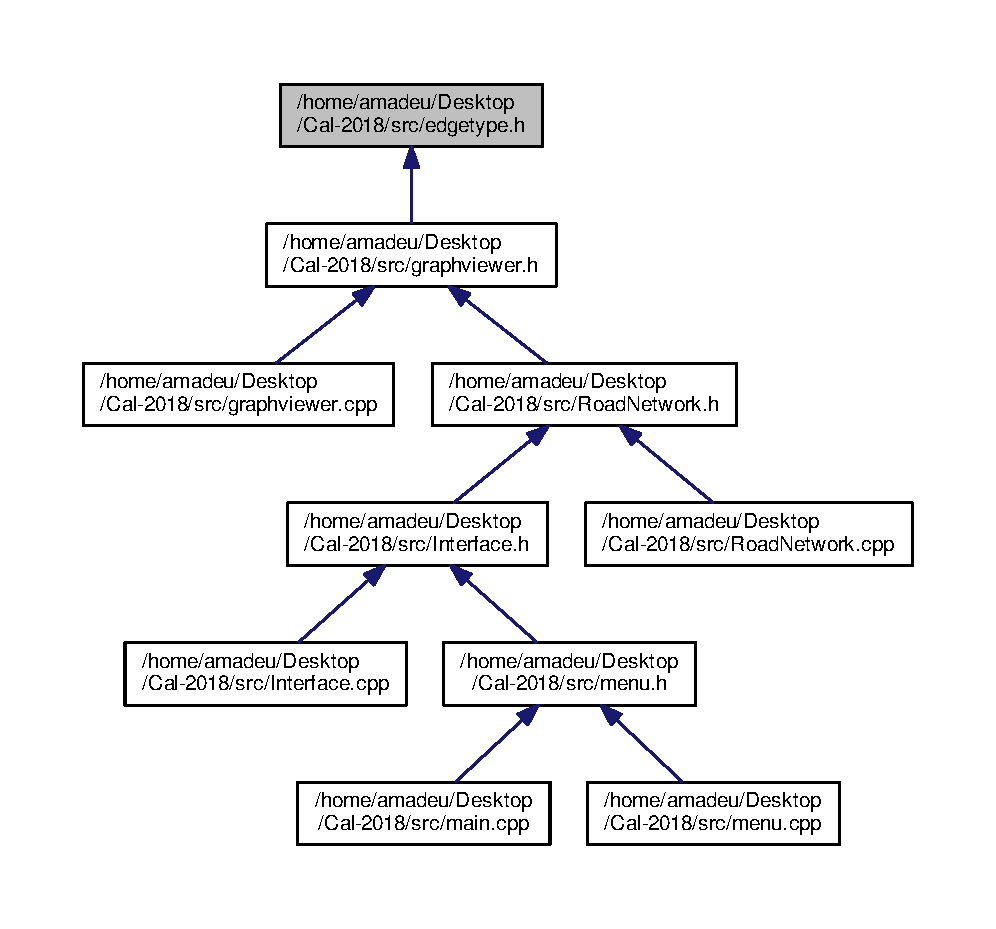
\includegraphics[width=350pt]{edgetype_8h__dep__incl}
\end{center}
\end{figure}
\subsection*{Classes}
\begin{DoxyCompactItemize}
\item 
class \hyperlink{classEdgeType}{Edge\+Type}
\end{DoxyCompactItemize}

\hypertarget{Graph_8h}{}\section{/home/amadeu/\+Desktop/\+Cal-\/2018/src/\+Graph.h File Reference}
\label{Graph_8h}\index{/home/amadeu/\+Desktop/\+Cal-\/2018/src/\+Graph.\+h@{/home/amadeu/\+Desktop/\+Cal-\/2018/src/\+Graph.\+h}}
{\ttfamily \#include $<$vector$>$}\\*
{\ttfamily \#include $<$queue$>$}\\*
{\ttfamily \#include $<$string$>$}\\*
{\ttfamily \#include $<$cmath$>$}\\*
{\ttfamily \#include $<$set$>$}\\*
{\ttfamily \#include $<$list$>$}\\*
{\ttfamily \#include $<$limits$>$}\\*
{\ttfamily \#include $<$climits$>$}\\*
{\ttfamily \#include \char`\"{}Mutable\+Priority\+Queue.\+h\char`\"{}}\\*
Include dependency graph for Graph.\+h\+:\nopagebreak
\begin{figure}[H]
\begin{center}
\leavevmode
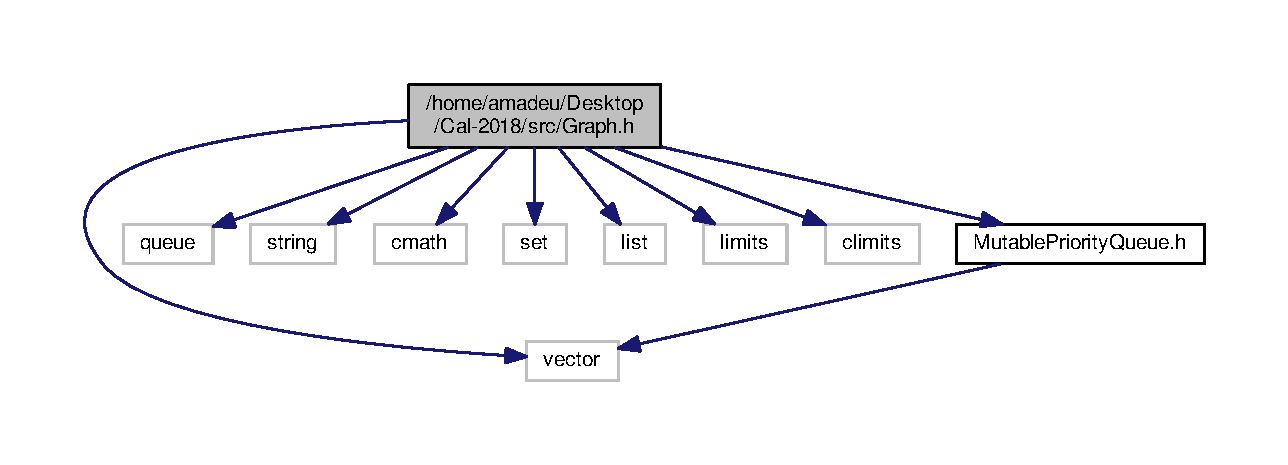
\includegraphics[width=350pt]{Graph_8h__incl}
\end{center}
\end{figure}
This graph shows which files directly or indirectly include this file\+:\nopagebreak
\begin{figure}[H]
\begin{center}
\leavevmode
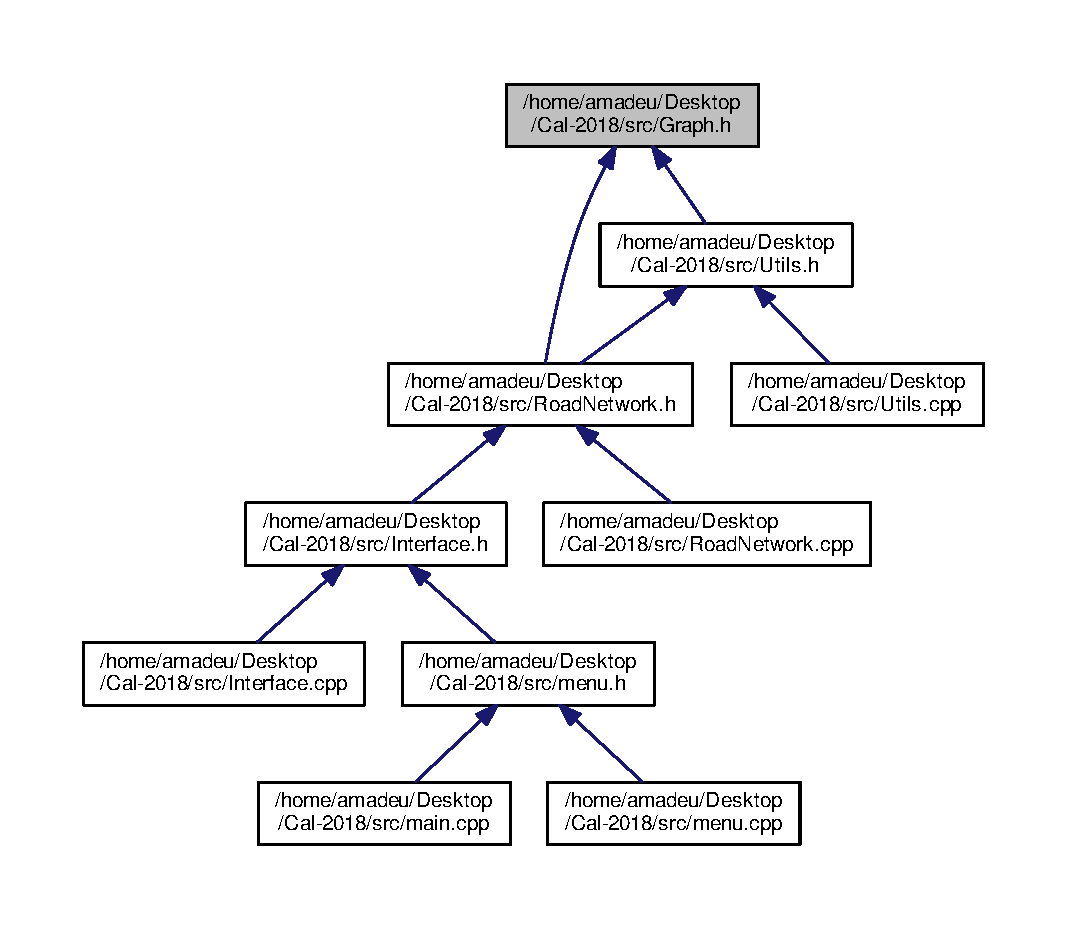
\includegraphics[width=350pt]{Graph_8h__dep__incl}
\end{center}
\end{figure}
\subsection*{Classes}
\begin{DoxyCompactItemize}
\item 
class \hyperlink{classEdge}{Edge$<$ T $>$}
\item 
class \hyperlink{classGraph}{Graph$<$ T $>$}
\item 
class \hyperlink{classVertex}{Vertex$<$ T $>$}
\item 
class \hyperlink{classCarro}{Carro$<$ T $>$}
\item 
class \hyperlink{classCarro}{Carro$<$ T $>$}
\item 
class \hyperlink{classVertex}{Vertex$<$ T $>$}
\item 
struct \hyperlink{structvertex__greater__than}{vertex\+\_\+greater\+\_\+than$<$ T $>$}
\item 
class \hyperlink{classEdge}{Edge$<$ T $>$}
\item 
class \hyperlink{classGraph}{Graph$<$ T $>$}
\end{DoxyCompactItemize}
\subsection*{Macros}
\begin{DoxyCompactItemize}
\item 
\#define \hyperlink{Graph_8h_a12c2040f25d8e3a7b9e1c2024c618cb6}{I\+NF}~std\+::numeric\+\_\+limits$<$double$>$\+::max()
\item 
\#define \hyperlink{Graph_8h_abc29155cbf8d3ba92a8cb487bbabdc66}{M\+A\+X\+\_\+\+C\+A\+P\+A\+C\+I\+TY}~10
\end{DoxyCompactItemize}


\subsection{Macro Definition Documentation}
\index{Graph.\+h@{Graph.\+h}!I\+NF@{I\+NF}}
\index{I\+NF@{I\+NF}!Graph.\+h@{Graph.\+h}}
\subsubsection[{\texorpdfstring{I\+NF}{INF}}]{\setlength{\rightskip}{0pt plus 5cm}\#define I\+NF~std\+::numeric\+\_\+limits$<$double$>$\+::max()}\hypertarget{Graph_8h_a12c2040f25d8e3a7b9e1c2024c618cb6}{}\label{Graph_8h_a12c2040f25d8e3a7b9e1c2024c618cb6}
\index{Graph.\+h@{Graph.\+h}!M\+A\+X\+\_\+\+C\+A\+P\+A\+C\+I\+TY@{M\+A\+X\+\_\+\+C\+A\+P\+A\+C\+I\+TY}}
\index{M\+A\+X\+\_\+\+C\+A\+P\+A\+C\+I\+TY@{M\+A\+X\+\_\+\+C\+A\+P\+A\+C\+I\+TY}!Graph.\+h@{Graph.\+h}}
\subsubsection[{\texorpdfstring{M\+A\+X\+\_\+\+C\+A\+P\+A\+C\+I\+TY}{MAX_CAPACITY}}]{\setlength{\rightskip}{0pt plus 5cm}\#define M\+A\+X\+\_\+\+C\+A\+P\+A\+C\+I\+TY~10}\hypertarget{Graph_8h_abc29155cbf8d3ba92a8cb487bbabdc66}{}\label{Graph_8h_abc29155cbf8d3ba92a8cb487bbabdc66}
Capacidade maxima das arestas 
\hypertarget{graphviewer_8cpp}{}\section{/\+Users/amadeuppereira/\+F\+E\+U\+P/2ano/\+Cal-\/2018/src/graphviewer.cpp File Reference}
\label{graphviewer_8cpp}\index{/\+Users/amadeuppereira/\+F\+E\+U\+P/2ano/\+Cal-\/2018/src/graphviewer.\+cpp@{/\+Users/amadeuppereira/\+F\+E\+U\+P/2ano/\+Cal-\/2018/src/graphviewer.\+cpp}}
{\ttfamily \#include \char`\"{}graphviewer.\+h\char`\"{}}\newline
{\ttfamily \#include $<$string$>$}\newline
{\ttfamily \#include $<$sstream$>$}\newline

\hypertarget{graphviewer_8h}{}\section{/home/amadeu/\+Desktop/\+Cal-\/2018/src/graphviewer.h File Reference}
\label{graphviewer_8h}\index{/home/amadeu/\+Desktop/\+Cal-\/2018/src/graphviewer.\+h@{/home/amadeu/\+Desktop/\+Cal-\/2018/src/graphviewer.\+h}}
{\ttfamily \#include $<$winsock2.\+h$>$}\\*
{\ttfamily \#include $<$Windows.\+h$>$}\\*
{\ttfamily \#include $<$stdlib.\+h$>$}\\*
{\ttfamily \#include $<$signal.\+h$>$}\\*
{\ttfamily \#include $<$string$>$}\\*
{\ttfamily \#include \char`\"{}edgetype.\+h\char`\"{}}\\*
{\ttfamily \#include \char`\"{}connection.\+h\char`\"{}}\\*
Include dependency graph for graphviewer.\+h\+:\nopagebreak
\begin{figure}[H]
\begin{center}
\leavevmode
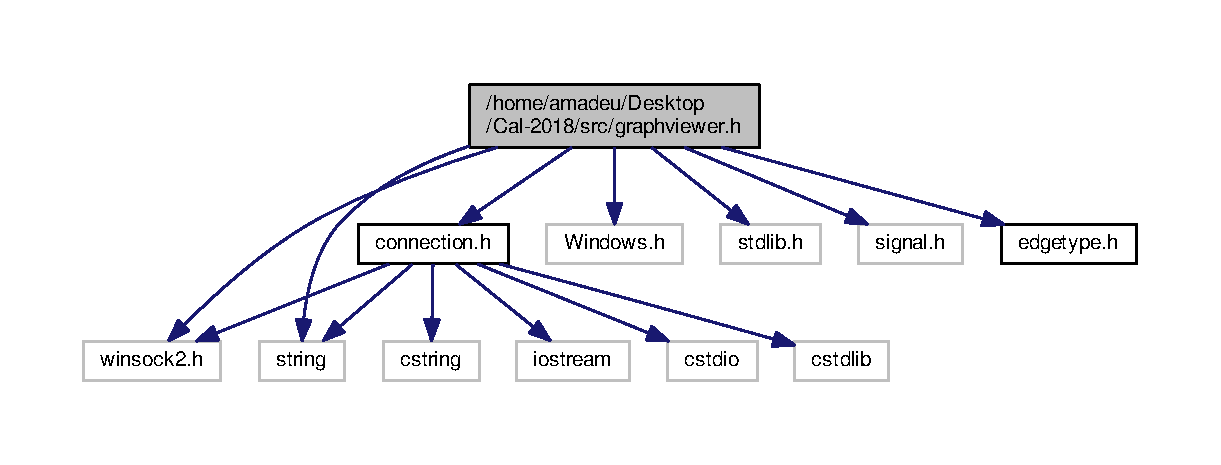
\includegraphics[width=350pt]{graphviewer_8h__incl}
\end{center}
\end{figure}
This graph shows which files directly or indirectly include this file\+:\nopagebreak
\begin{figure}[H]
\begin{center}
\leavevmode
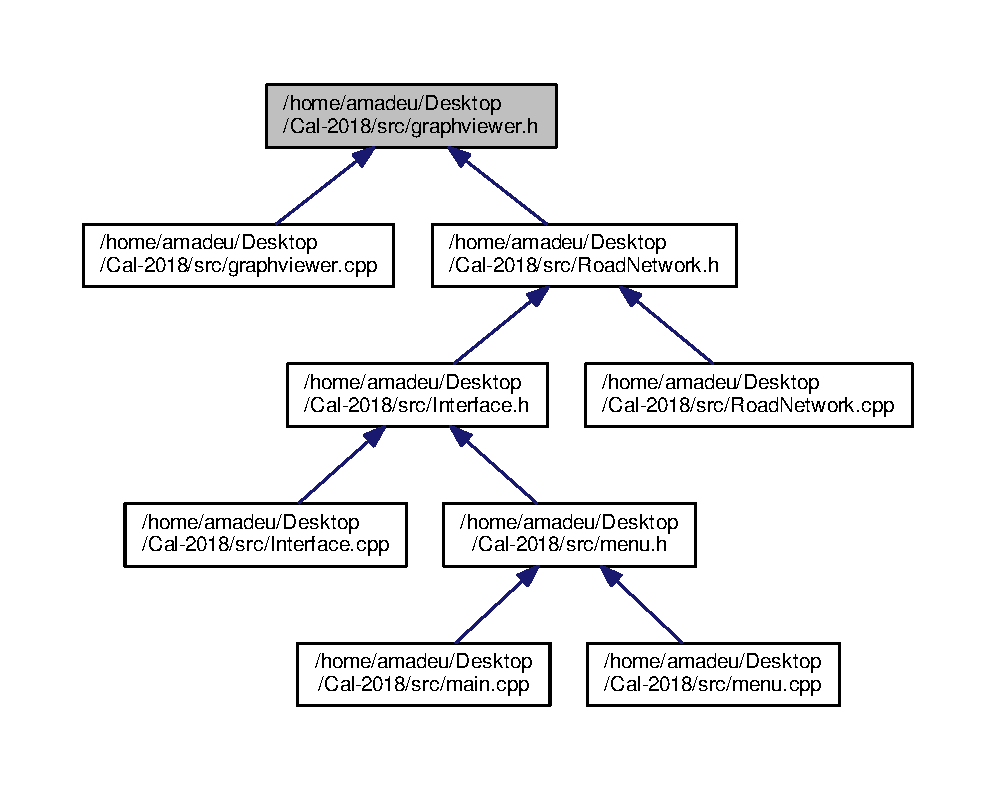
\includegraphics[width=350pt]{graphviewer_8h__dep__incl}
\end{center}
\end{figure}
\subsection*{Classes}
\begin{DoxyCompactItemize}
\item 
class \hyperlink{classGraphViewer}{Graph\+Viewer}
\end{DoxyCompactItemize}
\subsection*{Macros}
\begin{DoxyCompactItemize}
\item 
\#define \hyperlink{graphviewer_8h_a79d10e672abb49ad63eeaa8aaef57c38}{B\+L\+UE}~\char`\"{}B\+L\+UE\char`\"{}
\item 
\#define \hyperlink{graphviewer_8h_a8d23feea868a983c8c2b661e1e16972f}{R\+ED}~\char`\"{}R\+ED\char`\"{}
\item 
\#define \hyperlink{graphviewer_8h_ada419fe3b48fcf19daed7cc57ccf1174}{P\+I\+NK}~\char`\"{}P\+I\+NK\char`\"{}
\item 
\#define \hyperlink{graphviewer_8h_a7b3b25cba33b07c303f3060fe41887f6}{B\+L\+A\+CK}~\char`\"{}B\+L\+A\+CK\char`\"{}
\item 
\#define \hyperlink{graphviewer_8h_a87b537f5fa5c109d3c05c13d6b18f382}{W\+H\+I\+TE}~\char`\"{}W\+H\+I\+TE\char`\"{}
\item 
\#define \hyperlink{graphviewer_8h_ac5b6e19bf06822021f35602c59658de3}{O\+R\+A\+N\+GE}~\char`\"{}O\+R\+A\+N\+GE\char`\"{}
\item 
\#define \hyperlink{graphviewer_8h_abf681265909adf3d3e8116c93c0ba179}{Y\+E\+L\+L\+OW}~\char`\"{}Y\+E\+L\+L\+OW\char`\"{}
\item 
\#define \hyperlink{graphviewer_8h_acfbc006ea433ad708fdee3e82996e721}{G\+R\+E\+EN}~\char`\"{}G\+R\+E\+EN\char`\"{}
\item 
\#define \hyperlink{graphviewer_8h_ad243f93c16bc4c1d3e0a13b84421d760}{C\+Y\+AN}~\char`\"{}C\+Y\+AN\char`\"{}
\item 
\#define \hyperlink{graphviewer_8h_ae5f70677050eecd8909e0248e07b9e73}{G\+R\+AY}~\char`\"{}G\+R\+AY\char`\"{}
\item 
\#define \hyperlink{graphviewer_8h_aca56870f2285abae489635f0ee4d65e3}{D\+A\+R\+K\+\_\+\+G\+R\+AY}~\char`\"{}D\+A\+R\+K\+\_\+\+G\+R\+AY\char`\"{}
\item 
\#define \hyperlink{graphviewer_8h_a9663e02e20b5b578e6a31adae265cb88}{L\+I\+G\+H\+T\+\_\+\+G\+R\+AY}~\char`\"{}L\+I\+G\+H\+T\+\_\+\+G\+R\+AY\char`\"{}
\item 
\#define \hyperlink{graphviewer_8h_a6f699060902f800f12aaae150f3a708e}{M\+A\+G\+E\+N\+TA}~\char`\"{}M\+A\+G\+E\+N\+TA\char`\"{}
\end{DoxyCompactItemize}


\subsection{Macro Definition Documentation}
\index{graphviewer.\+h@{graphviewer.\+h}!B\+L\+A\+CK@{B\+L\+A\+CK}}
\index{B\+L\+A\+CK@{B\+L\+A\+CK}!graphviewer.\+h@{graphviewer.\+h}}
\subsubsection[{\texorpdfstring{B\+L\+A\+CK}{BLACK}}]{\setlength{\rightskip}{0pt plus 5cm}\#define B\+L\+A\+CK~\char`\"{}B\+L\+A\+CK\char`\"{}}\hypertarget{graphviewer_8h_a7b3b25cba33b07c303f3060fe41887f6}{}\label{graphviewer_8h_a7b3b25cba33b07c303f3060fe41887f6}
\index{graphviewer.\+h@{graphviewer.\+h}!B\+L\+UE@{B\+L\+UE}}
\index{B\+L\+UE@{B\+L\+UE}!graphviewer.\+h@{graphviewer.\+h}}
\subsubsection[{\texorpdfstring{B\+L\+UE}{BLUE}}]{\setlength{\rightskip}{0pt plus 5cm}\#define B\+L\+UE~\char`\"{}B\+L\+UE\char`\"{}}\hypertarget{graphviewer_8h_a79d10e672abb49ad63eeaa8aaef57c38}{}\label{graphviewer_8h_a79d10e672abb49ad63eeaa8aaef57c38}
\index{graphviewer.\+h@{graphviewer.\+h}!C\+Y\+AN@{C\+Y\+AN}}
\index{C\+Y\+AN@{C\+Y\+AN}!graphviewer.\+h@{graphviewer.\+h}}
\subsubsection[{\texorpdfstring{C\+Y\+AN}{CYAN}}]{\setlength{\rightskip}{0pt plus 5cm}\#define C\+Y\+AN~\char`\"{}C\+Y\+AN\char`\"{}}\hypertarget{graphviewer_8h_ad243f93c16bc4c1d3e0a13b84421d760}{}\label{graphviewer_8h_ad243f93c16bc4c1d3e0a13b84421d760}
\index{graphviewer.\+h@{graphviewer.\+h}!D\+A\+R\+K\+\_\+\+G\+R\+AY@{D\+A\+R\+K\+\_\+\+G\+R\+AY}}
\index{D\+A\+R\+K\+\_\+\+G\+R\+AY@{D\+A\+R\+K\+\_\+\+G\+R\+AY}!graphviewer.\+h@{graphviewer.\+h}}
\subsubsection[{\texorpdfstring{D\+A\+R\+K\+\_\+\+G\+R\+AY}{DARK_GRAY}}]{\setlength{\rightskip}{0pt plus 5cm}\#define D\+A\+R\+K\+\_\+\+G\+R\+AY~\char`\"{}D\+A\+R\+K\+\_\+\+G\+R\+AY\char`\"{}}\hypertarget{graphviewer_8h_aca56870f2285abae489635f0ee4d65e3}{}\label{graphviewer_8h_aca56870f2285abae489635f0ee4d65e3}
\index{graphviewer.\+h@{graphviewer.\+h}!G\+R\+AY@{G\+R\+AY}}
\index{G\+R\+AY@{G\+R\+AY}!graphviewer.\+h@{graphviewer.\+h}}
\subsubsection[{\texorpdfstring{G\+R\+AY}{GRAY}}]{\setlength{\rightskip}{0pt plus 5cm}\#define G\+R\+AY~\char`\"{}G\+R\+AY\char`\"{}}\hypertarget{graphviewer_8h_ae5f70677050eecd8909e0248e07b9e73}{}\label{graphviewer_8h_ae5f70677050eecd8909e0248e07b9e73}
\index{graphviewer.\+h@{graphviewer.\+h}!G\+R\+E\+EN@{G\+R\+E\+EN}}
\index{G\+R\+E\+EN@{G\+R\+E\+EN}!graphviewer.\+h@{graphviewer.\+h}}
\subsubsection[{\texorpdfstring{G\+R\+E\+EN}{GREEN}}]{\setlength{\rightskip}{0pt plus 5cm}\#define G\+R\+E\+EN~\char`\"{}G\+R\+E\+EN\char`\"{}}\hypertarget{graphviewer_8h_acfbc006ea433ad708fdee3e82996e721}{}\label{graphviewer_8h_acfbc006ea433ad708fdee3e82996e721}
\index{graphviewer.\+h@{graphviewer.\+h}!L\+I\+G\+H\+T\+\_\+\+G\+R\+AY@{L\+I\+G\+H\+T\+\_\+\+G\+R\+AY}}
\index{L\+I\+G\+H\+T\+\_\+\+G\+R\+AY@{L\+I\+G\+H\+T\+\_\+\+G\+R\+AY}!graphviewer.\+h@{graphviewer.\+h}}
\subsubsection[{\texorpdfstring{L\+I\+G\+H\+T\+\_\+\+G\+R\+AY}{LIGHT_GRAY}}]{\setlength{\rightskip}{0pt plus 5cm}\#define L\+I\+G\+H\+T\+\_\+\+G\+R\+AY~\char`\"{}L\+I\+G\+H\+T\+\_\+\+G\+R\+AY\char`\"{}}\hypertarget{graphviewer_8h_a9663e02e20b5b578e6a31adae265cb88}{}\label{graphviewer_8h_a9663e02e20b5b578e6a31adae265cb88}
\index{graphviewer.\+h@{graphviewer.\+h}!M\+A\+G\+E\+N\+TA@{M\+A\+G\+E\+N\+TA}}
\index{M\+A\+G\+E\+N\+TA@{M\+A\+G\+E\+N\+TA}!graphviewer.\+h@{graphviewer.\+h}}
\subsubsection[{\texorpdfstring{M\+A\+G\+E\+N\+TA}{MAGENTA}}]{\setlength{\rightskip}{0pt plus 5cm}\#define M\+A\+G\+E\+N\+TA~\char`\"{}M\+A\+G\+E\+N\+TA\char`\"{}}\hypertarget{graphviewer_8h_a6f699060902f800f12aaae150f3a708e}{}\label{graphviewer_8h_a6f699060902f800f12aaae150f3a708e}
\index{graphviewer.\+h@{graphviewer.\+h}!O\+R\+A\+N\+GE@{O\+R\+A\+N\+GE}}
\index{O\+R\+A\+N\+GE@{O\+R\+A\+N\+GE}!graphviewer.\+h@{graphviewer.\+h}}
\subsubsection[{\texorpdfstring{O\+R\+A\+N\+GE}{ORANGE}}]{\setlength{\rightskip}{0pt plus 5cm}\#define O\+R\+A\+N\+GE~\char`\"{}O\+R\+A\+N\+GE\char`\"{}}\hypertarget{graphviewer_8h_ac5b6e19bf06822021f35602c59658de3}{}\label{graphviewer_8h_ac5b6e19bf06822021f35602c59658de3}
\index{graphviewer.\+h@{graphviewer.\+h}!P\+I\+NK@{P\+I\+NK}}
\index{P\+I\+NK@{P\+I\+NK}!graphviewer.\+h@{graphviewer.\+h}}
\subsubsection[{\texorpdfstring{P\+I\+NK}{PINK}}]{\setlength{\rightskip}{0pt plus 5cm}\#define P\+I\+NK~\char`\"{}P\+I\+NK\char`\"{}}\hypertarget{graphviewer_8h_ada419fe3b48fcf19daed7cc57ccf1174}{}\label{graphviewer_8h_ada419fe3b48fcf19daed7cc57ccf1174}
\index{graphviewer.\+h@{graphviewer.\+h}!R\+ED@{R\+ED}}
\index{R\+ED@{R\+ED}!graphviewer.\+h@{graphviewer.\+h}}
\subsubsection[{\texorpdfstring{R\+ED}{RED}}]{\setlength{\rightskip}{0pt plus 5cm}\#define R\+ED~\char`\"{}R\+ED\char`\"{}}\hypertarget{graphviewer_8h_a8d23feea868a983c8c2b661e1e16972f}{}\label{graphviewer_8h_a8d23feea868a983c8c2b661e1e16972f}
\index{graphviewer.\+h@{graphviewer.\+h}!W\+H\+I\+TE@{W\+H\+I\+TE}}
\index{W\+H\+I\+TE@{W\+H\+I\+TE}!graphviewer.\+h@{graphviewer.\+h}}
\subsubsection[{\texorpdfstring{W\+H\+I\+TE}{WHITE}}]{\setlength{\rightskip}{0pt plus 5cm}\#define W\+H\+I\+TE~\char`\"{}W\+H\+I\+TE\char`\"{}}\hypertarget{graphviewer_8h_a87b537f5fa5c109d3c05c13d6b18f382}{}\label{graphviewer_8h_a87b537f5fa5c109d3c05c13d6b18f382}
\index{graphviewer.\+h@{graphviewer.\+h}!Y\+E\+L\+L\+OW@{Y\+E\+L\+L\+OW}}
\index{Y\+E\+L\+L\+OW@{Y\+E\+L\+L\+OW}!graphviewer.\+h@{graphviewer.\+h}}
\subsubsection[{\texorpdfstring{Y\+E\+L\+L\+OW}{YELLOW}}]{\setlength{\rightskip}{0pt plus 5cm}\#define Y\+E\+L\+L\+OW~\char`\"{}Y\+E\+L\+L\+OW\char`\"{}}\hypertarget{graphviewer_8h_abf681265909adf3d3e8116c93c0ba179}{}\label{graphviewer_8h_abf681265909adf3d3e8116c93c0ba179}

\hypertarget{Interface_8cpp}{}\section{/home/amadeu/\+Desktop/\+Cal-\/2018/src/\+Interface.cpp File Reference}
\label{Interface_8cpp}\index{/home/amadeu/\+Desktop/\+Cal-\/2018/src/\+Interface.\+cpp@{/home/amadeu/\+Desktop/\+Cal-\/2018/src/\+Interface.\+cpp}}
{\ttfamily \#include \char`\"{}Interface.\+h\char`\"{}}\\*
Include dependency graph for Interface.\+cpp\+:\nopagebreak
\begin{figure}[H]
\begin{center}
\leavevmode
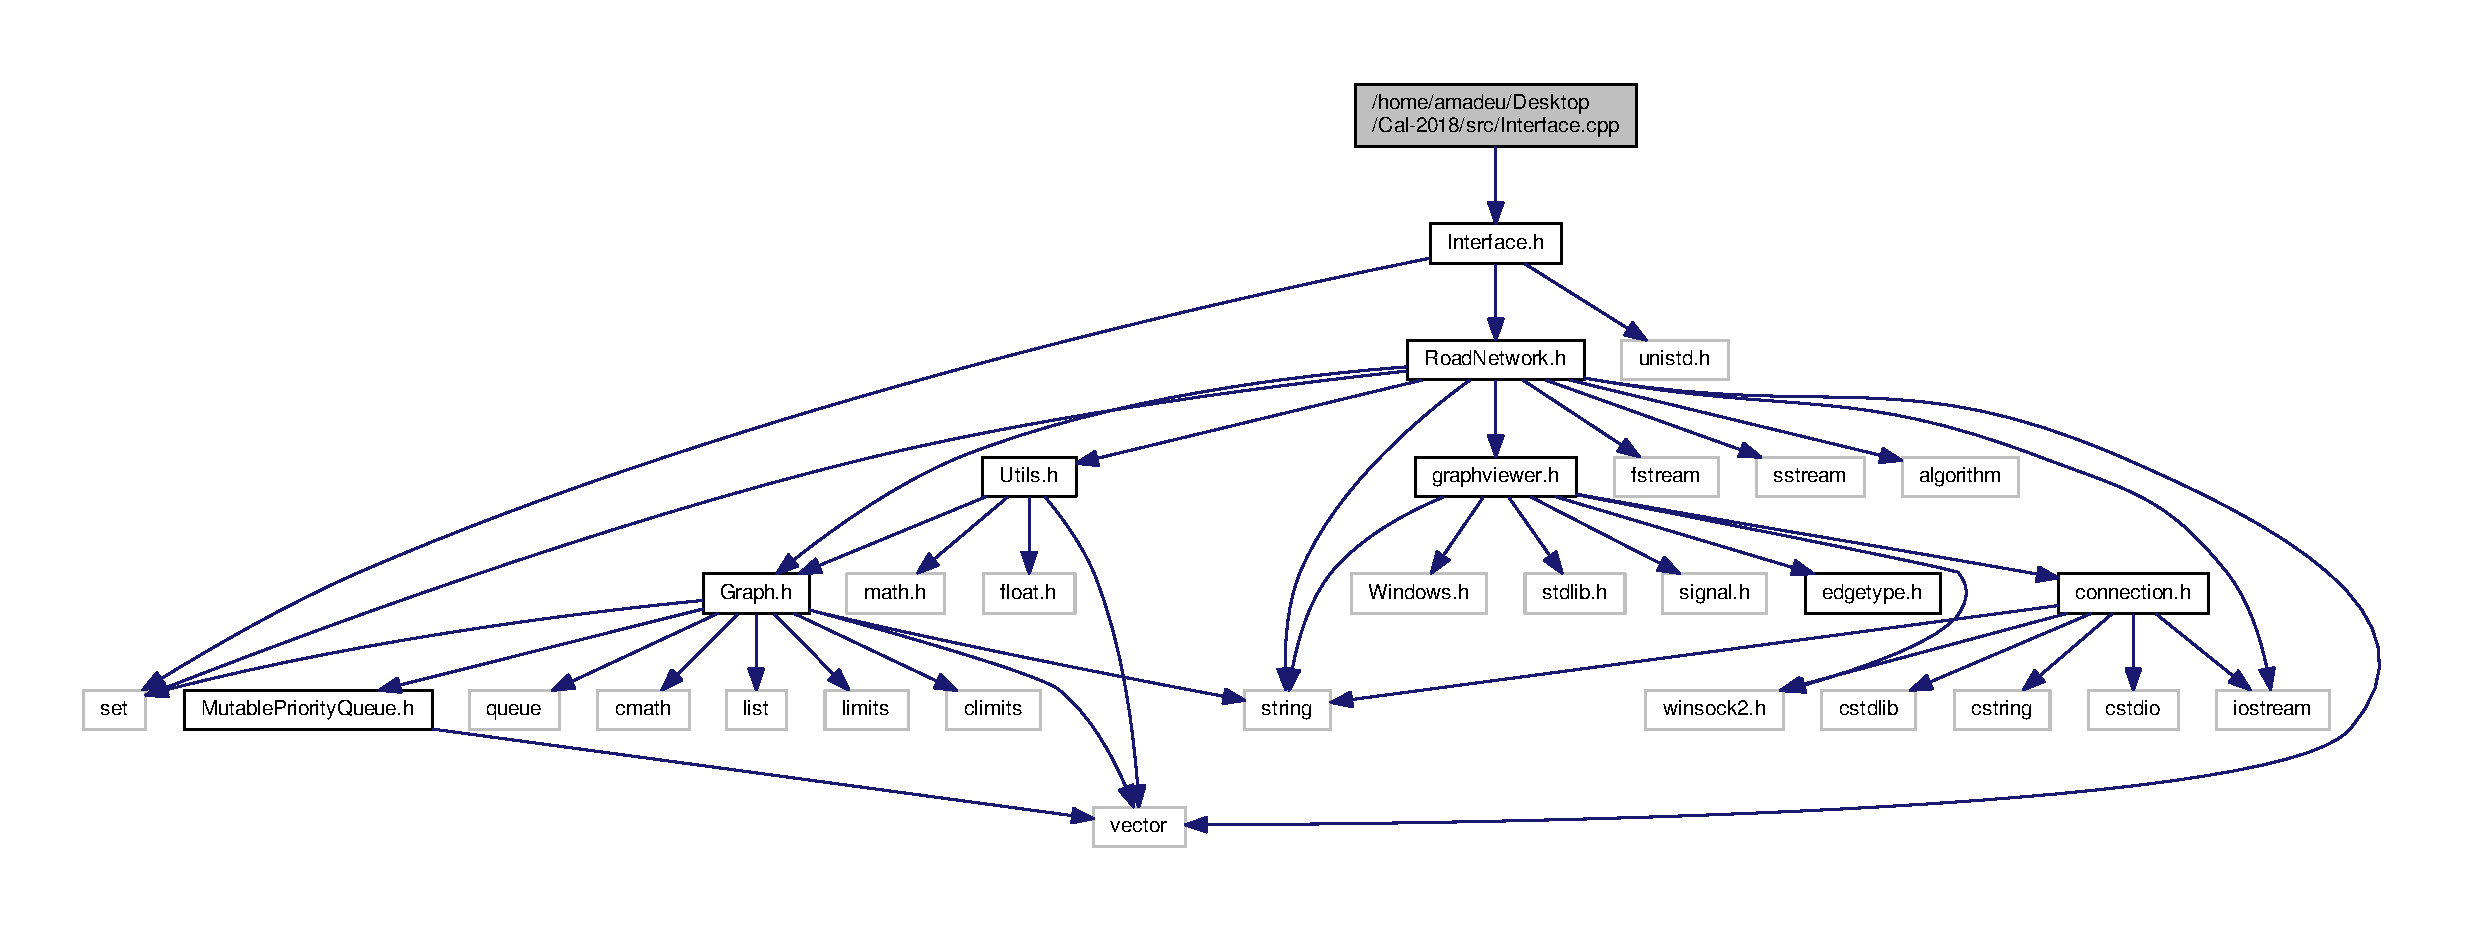
\includegraphics[width=350pt]{Interface_8cpp__incl}
\end{center}
\end{figure}

\hypertarget{Interface_8h}{}\section{/home/amadeu/\+Desktop/\+Cal-\/2018/src/\+Interface.h File Reference}
\label{Interface_8h}\index{/home/amadeu/\+Desktop/\+Cal-\/2018/src/\+Interface.\+h@{/home/amadeu/\+Desktop/\+Cal-\/2018/src/\+Interface.\+h}}
{\ttfamily \#include \char`\"{}Road\+Network.\+h\char`\"{}}\\*
{\ttfamily \#include $<$set$>$}\\*
{\ttfamily \#include $<$unistd.\+h$>$}\\*
Include dependency graph for Interface.\+h\+:\nopagebreak
\begin{figure}[H]
\begin{center}
\leavevmode
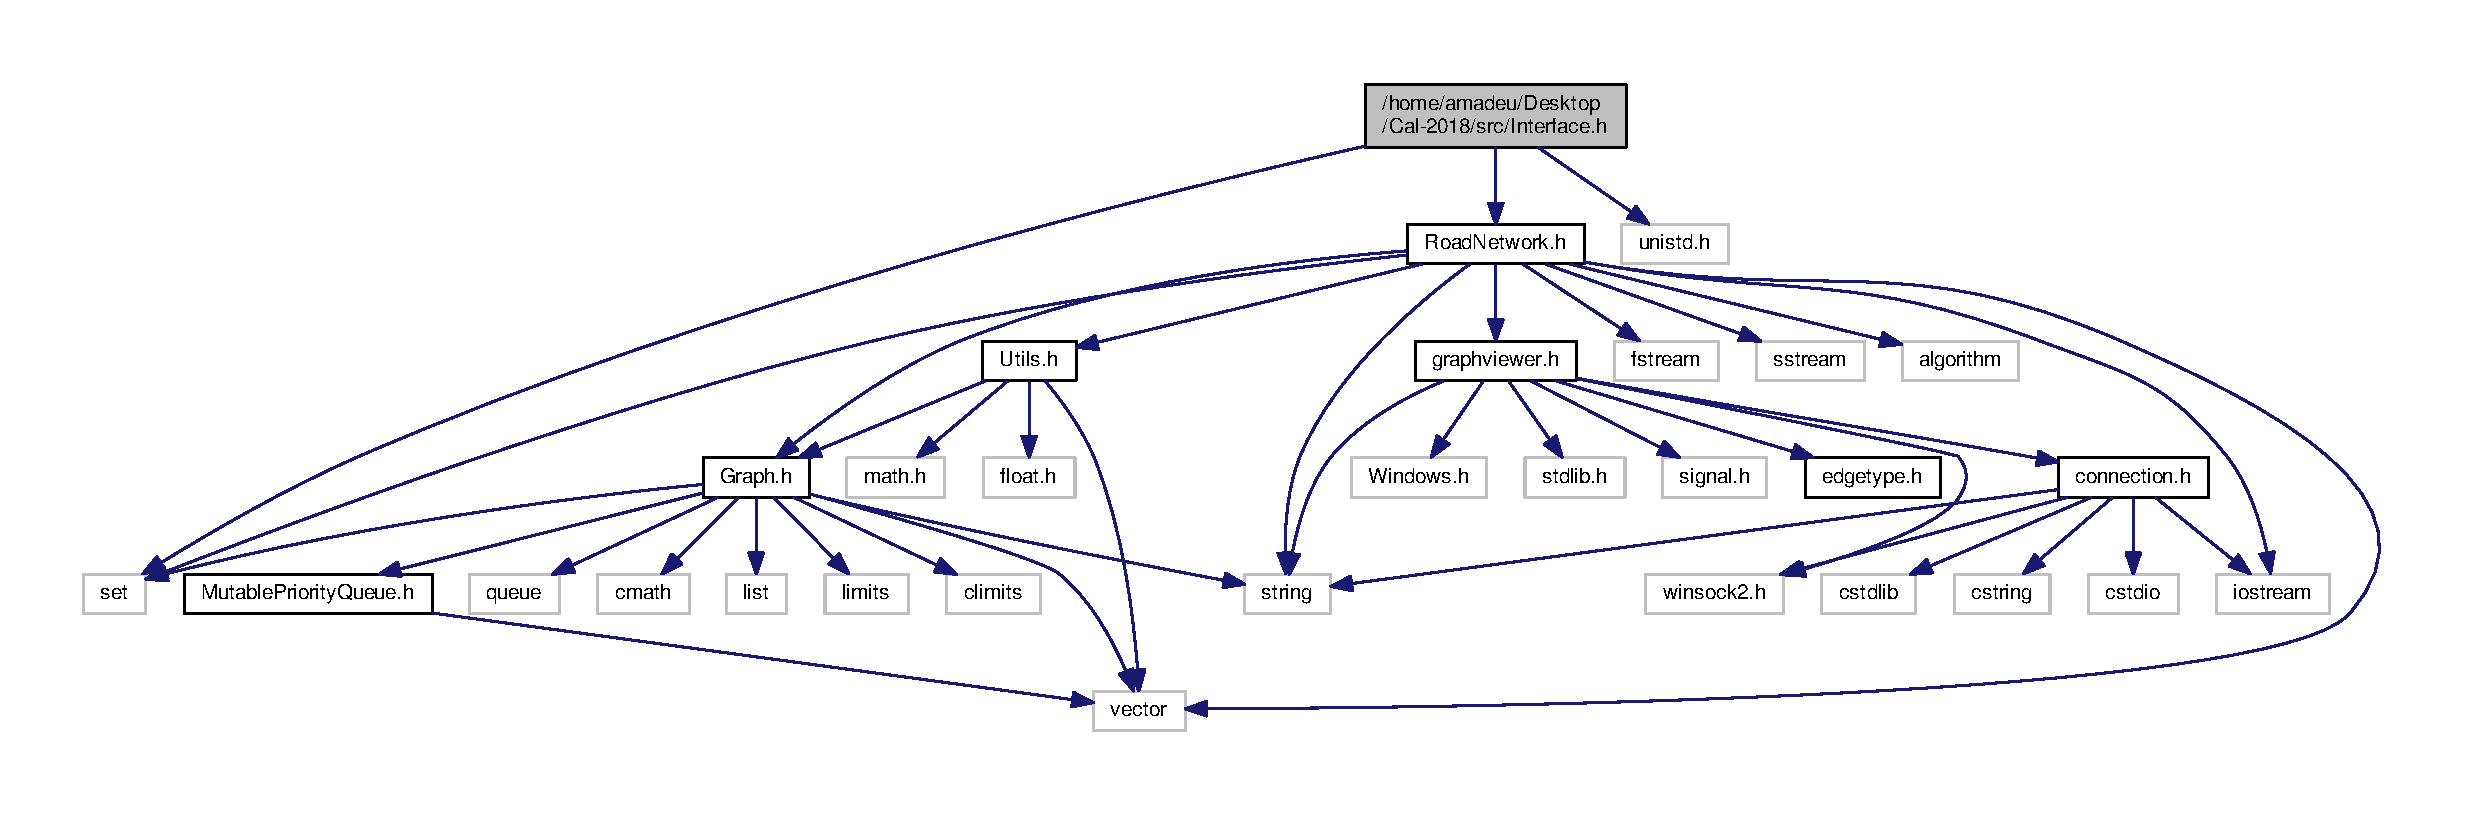
\includegraphics[width=350pt]{Interface_8h__incl}
\end{center}
\end{figure}
This graph shows which files directly or indirectly include this file\+:\nopagebreak
\begin{figure}[H]
\begin{center}
\leavevmode
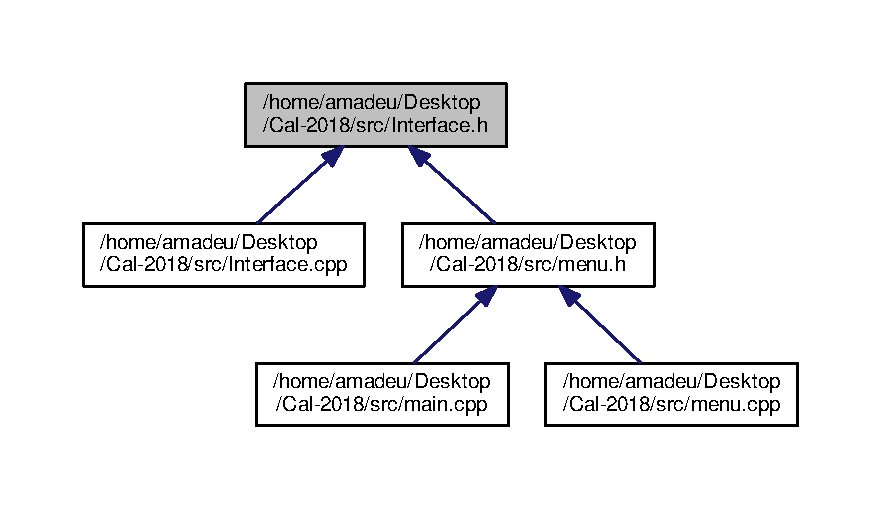
\includegraphics[width=350pt]{Interface_8h__dep__incl}
\end{center}
\end{figure}
\subsection*{Classes}
\begin{DoxyCompactItemize}
\item 
class \hyperlink{classInterface}{Interface}
\end{DoxyCompactItemize}

\hypertarget{main_8cpp}{}\section{/home/amadeu/\+Desktop/\+Cal-\/2018/src/main.cpp File Reference}
\label{main_8cpp}\index{/home/amadeu/\+Desktop/\+Cal-\/2018/src/main.\+cpp@{/home/amadeu/\+Desktop/\+Cal-\/2018/src/main.\+cpp}}
{\ttfamily \#include $<$iostream$>$}\\*
{\ttfamily \#include $<$string$>$}\\*
{\ttfamily \#include \char`\"{}menu.\+h\char`\"{}}\\*
Include dependency graph for main.\+cpp\+:\nopagebreak
\begin{figure}[H]
\begin{center}
\leavevmode
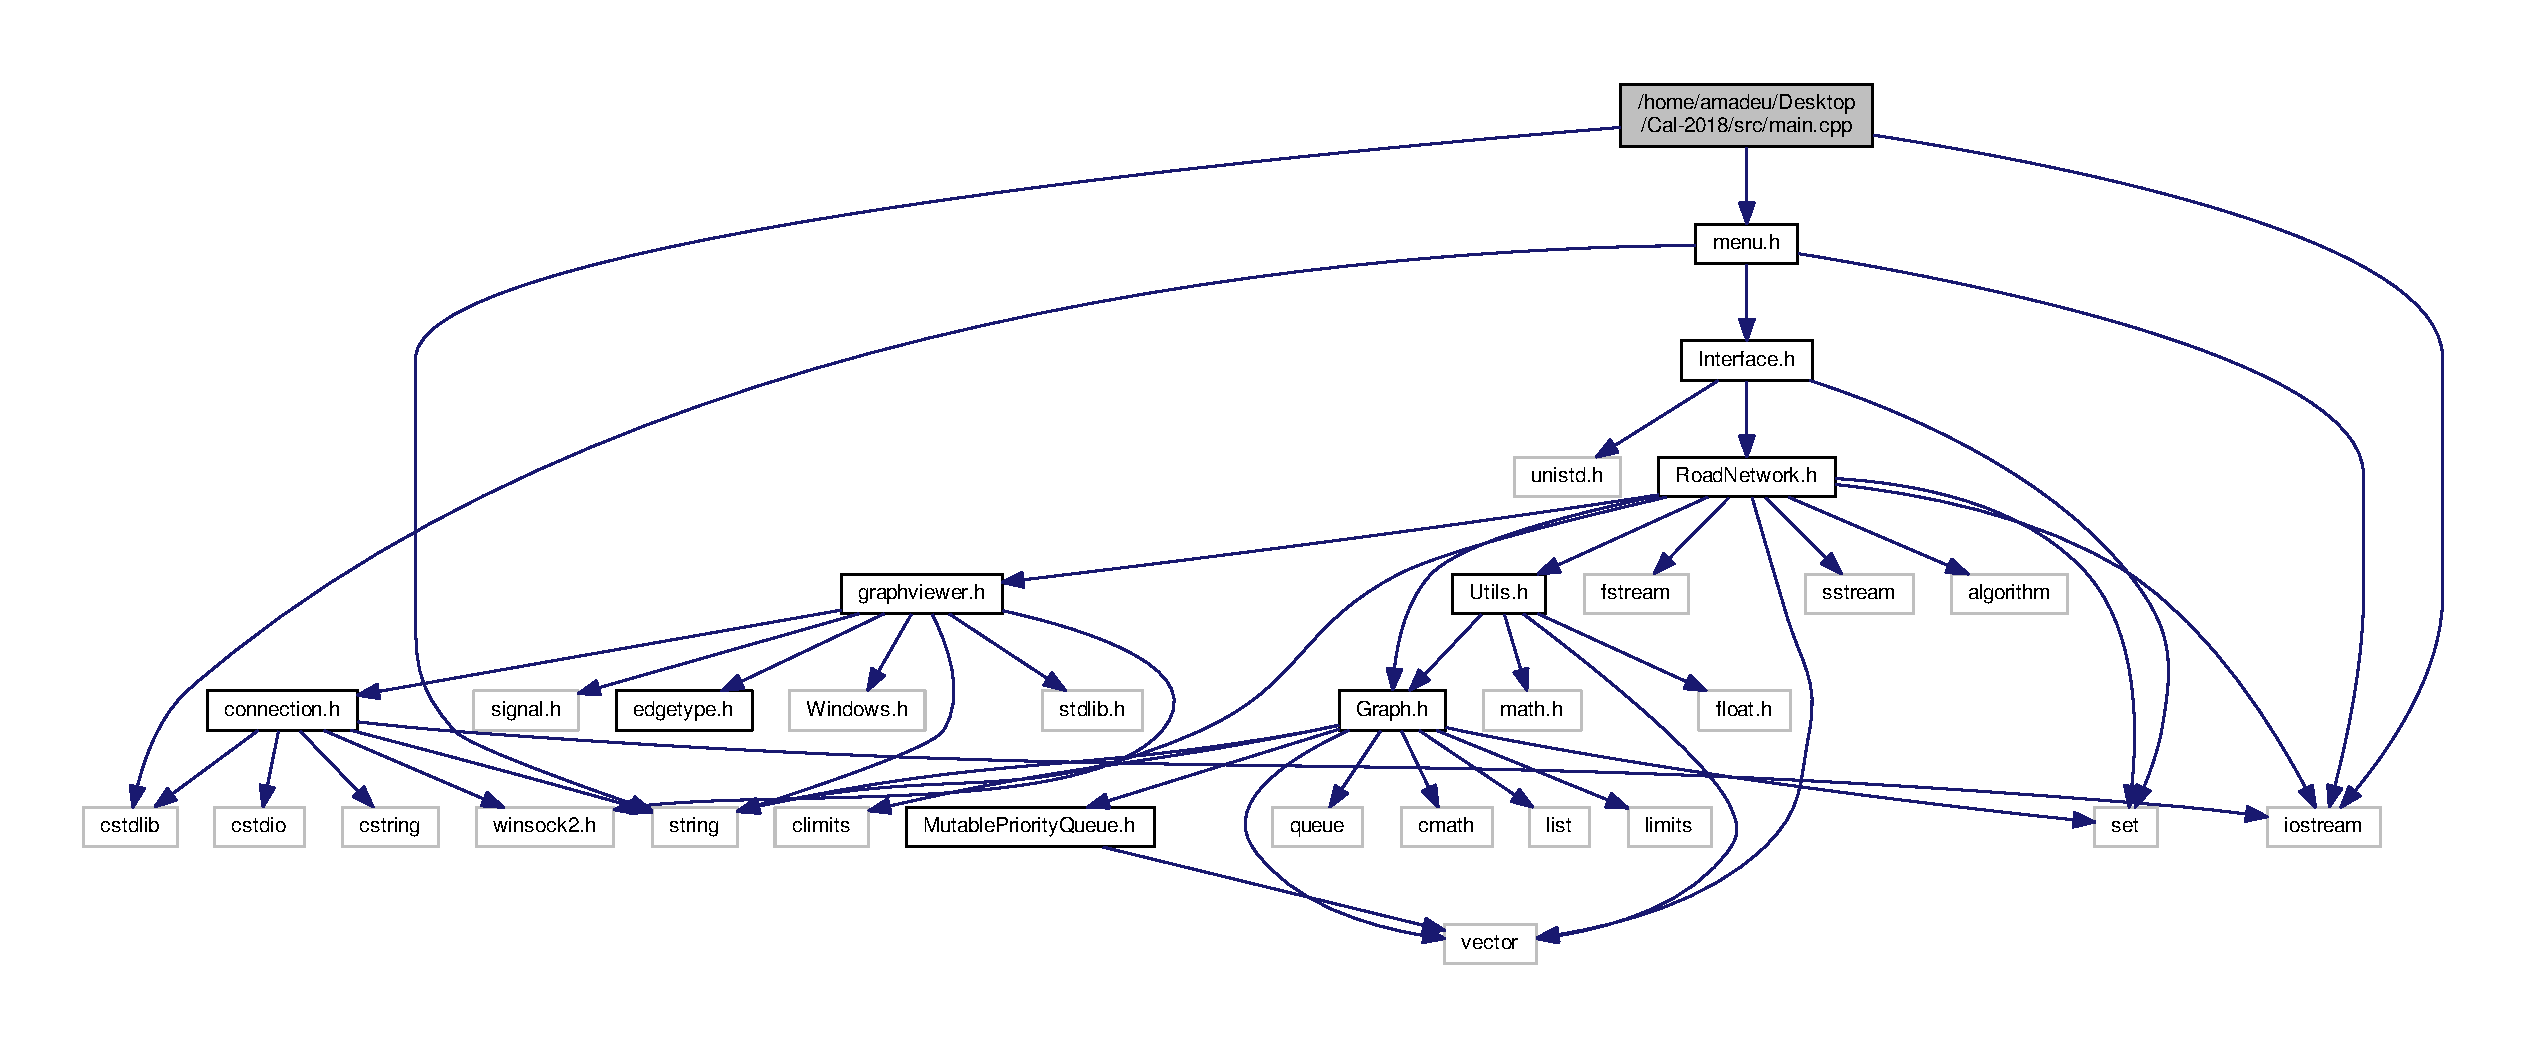
\includegraphics[width=350pt]{main_8cpp__incl}
\end{center}
\end{figure}
\subsection*{Functions}
\begin{DoxyCompactItemize}
\item 
int \hyperlink{main_8cpp_ae66f6b31b5ad750f1fe042a706a4e3d4}{main} ()
\end{DoxyCompactItemize}


\subsection{Function Documentation}
\index{main.\+cpp@{main.\+cpp}!main@{main}}
\index{main@{main}!main.\+cpp@{main.\+cpp}}
\subsubsection[{\texorpdfstring{main()}{main()}}]{\setlength{\rightskip}{0pt plus 5cm}int main (
\begin{DoxyParamCaption}
{}
\end{DoxyParamCaption}
)}\hypertarget{main_8cpp_ae66f6b31b5ad750f1fe042a706a4e3d4}{}\label{main_8cpp_ae66f6b31b5ad750f1fe042a706a4e3d4}

\hypertarget{menu_8cpp}{}\section{/home/amadeu/\+Desktop/\+Cal-\/2018/src/menu.cpp File Reference}
\label{menu_8cpp}\index{/home/amadeu/\+Desktop/\+Cal-\/2018/src/menu.\+cpp@{/home/amadeu/\+Desktop/\+Cal-\/2018/src/menu.\+cpp}}
{\ttfamily \#include \char`\"{}menu.\+h\char`\"{}}\\*
Include dependency graph for menu.\+cpp\+:\nopagebreak
\begin{figure}[H]
\begin{center}
\leavevmode
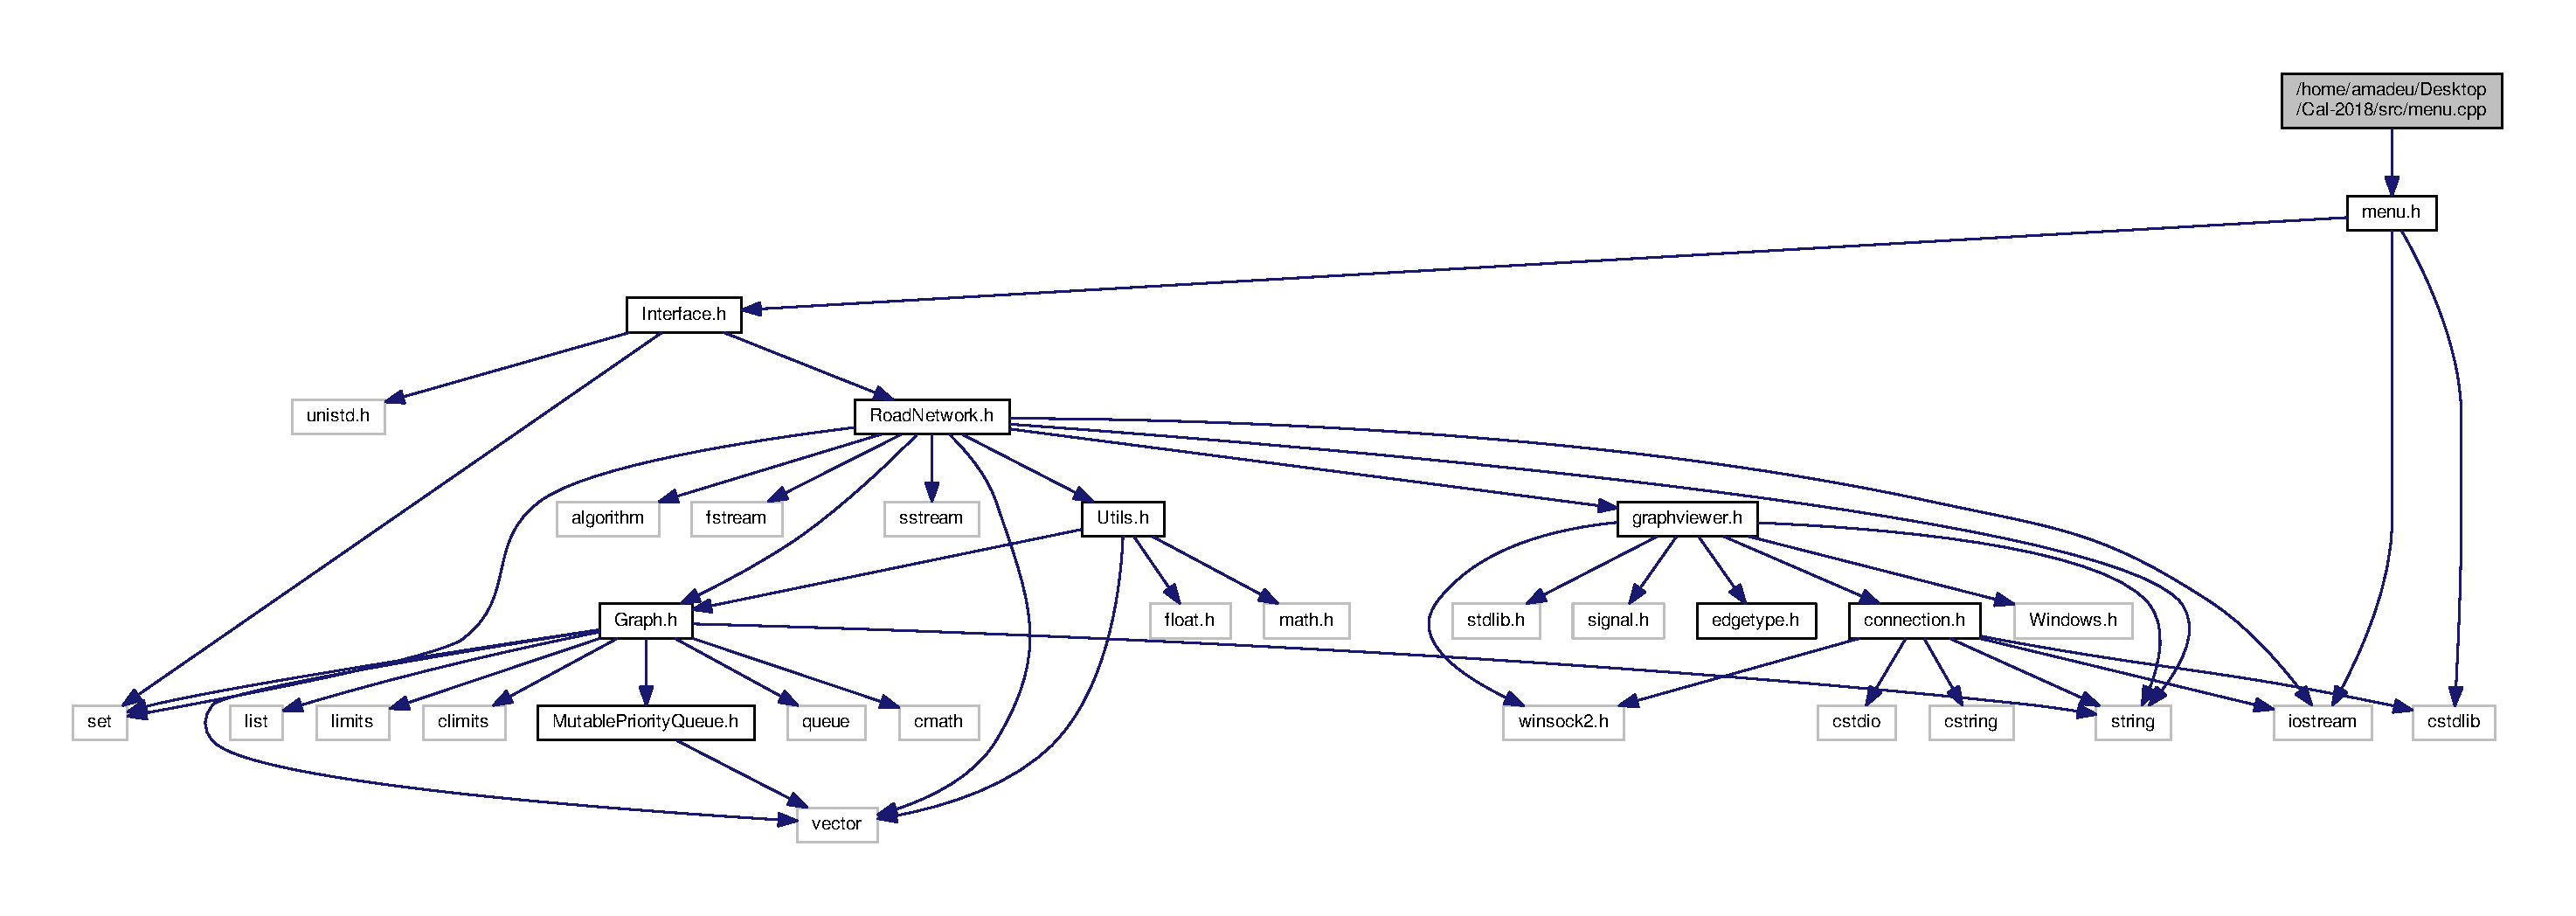
\includegraphics[width=350pt]{menu_8cpp__incl}
\end{center}
\end{figure}
\subsection*{Functions}
\begin{DoxyCompactItemize}
\item 
void \hyperlink{menu_8cpp_ae3e62f59c2eb3d57ecc15606da4a7c20}{save\+Files} ()
\item 
void \hyperlink{menu_8cpp_a2a0e843767aeea4f433a28b9c54f573a}{menu} ()
\end{DoxyCompactItemize}
\subsection*{Variables}
\begin{DoxyCompactItemize}
\item 
static \hyperlink{classInterface}{Interface} \hyperlink{menu_8cpp_a98862a04b438a5359a542f245ca97b62}{i} = \hyperlink{classInterface}{Interface}()
\end{DoxyCompactItemize}


\subsection{Function Documentation}
\index{menu.\+cpp@{menu.\+cpp}!menu@{menu}}
\index{menu@{menu}!menu.\+cpp@{menu.\+cpp}}
\subsubsection[{\texorpdfstring{menu()}{menu()}}]{\setlength{\rightskip}{0pt plus 5cm}void menu (
\begin{DoxyParamCaption}
{}
\end{DoxyParamCaption}
)}\hypertarget{menu_8cpp_a2a0e843767aeea4f433a28b9c54f573a}{}\label{menu_8cpp_a2a0e843767aeea4f433a28b9c54f573a}
Menu do programa \index{menu.\+cpp@{menu.\+cpp}!save\+Files@{save\+Files}}
\index{save\+Files@{save\+Files}!menu.\+cpp@{menu.\+cpp}}
\subsubsection[{\texorpdfstring{save\+Files()}{saveFiles()}}]{\setlength{\rightskip}{0pt plus 5cm}void save\+Files (
\begin{DoxyParamCaption}
{}
\end{DoxyParamCaption}
)}\hypertarget{menu_8cpp_ae3e62f59c2eb3d57ecc15606da4a7c20}{}\label{menu_8cpp_ae3e62f59c2eb3d57ecc15606da4a7c20}


\subsection{Variable Documentation}
\index{menu.\+cpp@{menu.\+cpp}!i@{i}}
\index{i@{i}!menu.\+cpp@{menu.\+cpp}}
\subsubsection[{\texorpdfstring{i}{i}}]{\setlength{\rightskip}{0pt plus 5cm}{\bf Interface} i = {\bf Interface}()\hspace{0.3cm}{\ttfamily [static]}}\hypertarget{menu_8cpp_a98862a04b438a5359a542f245ca97b62}{}\label{menu_8cpp_a98862a04b438a5359a542f245ca97b62}

\hypertarget{menu_8h}{}\section{/home/amadeu/\+Desktop/\+Cal-\/2018/src/menu.h File Reference}
\label{menu_8h}\index{/home/amadeu/\+Desktop/\+Cal-\/2018/src/menu.\+h@{/home/amadeu/\+Desktop/\+Cal-\/2018/src/menu.\+h}}
{\ttfamily \#include $<$iostream$>$}\\*
{\ttfamily \#include $<$cstdlib$>$}\\*
{\ttfamily \#include \char`\"{}Interface.\+h\char`\"{}}\\*
Include dependency graph for menu.\+h\+:\nopagebreak
\begin{figure}[H]
\begin{center}
\leavevmode
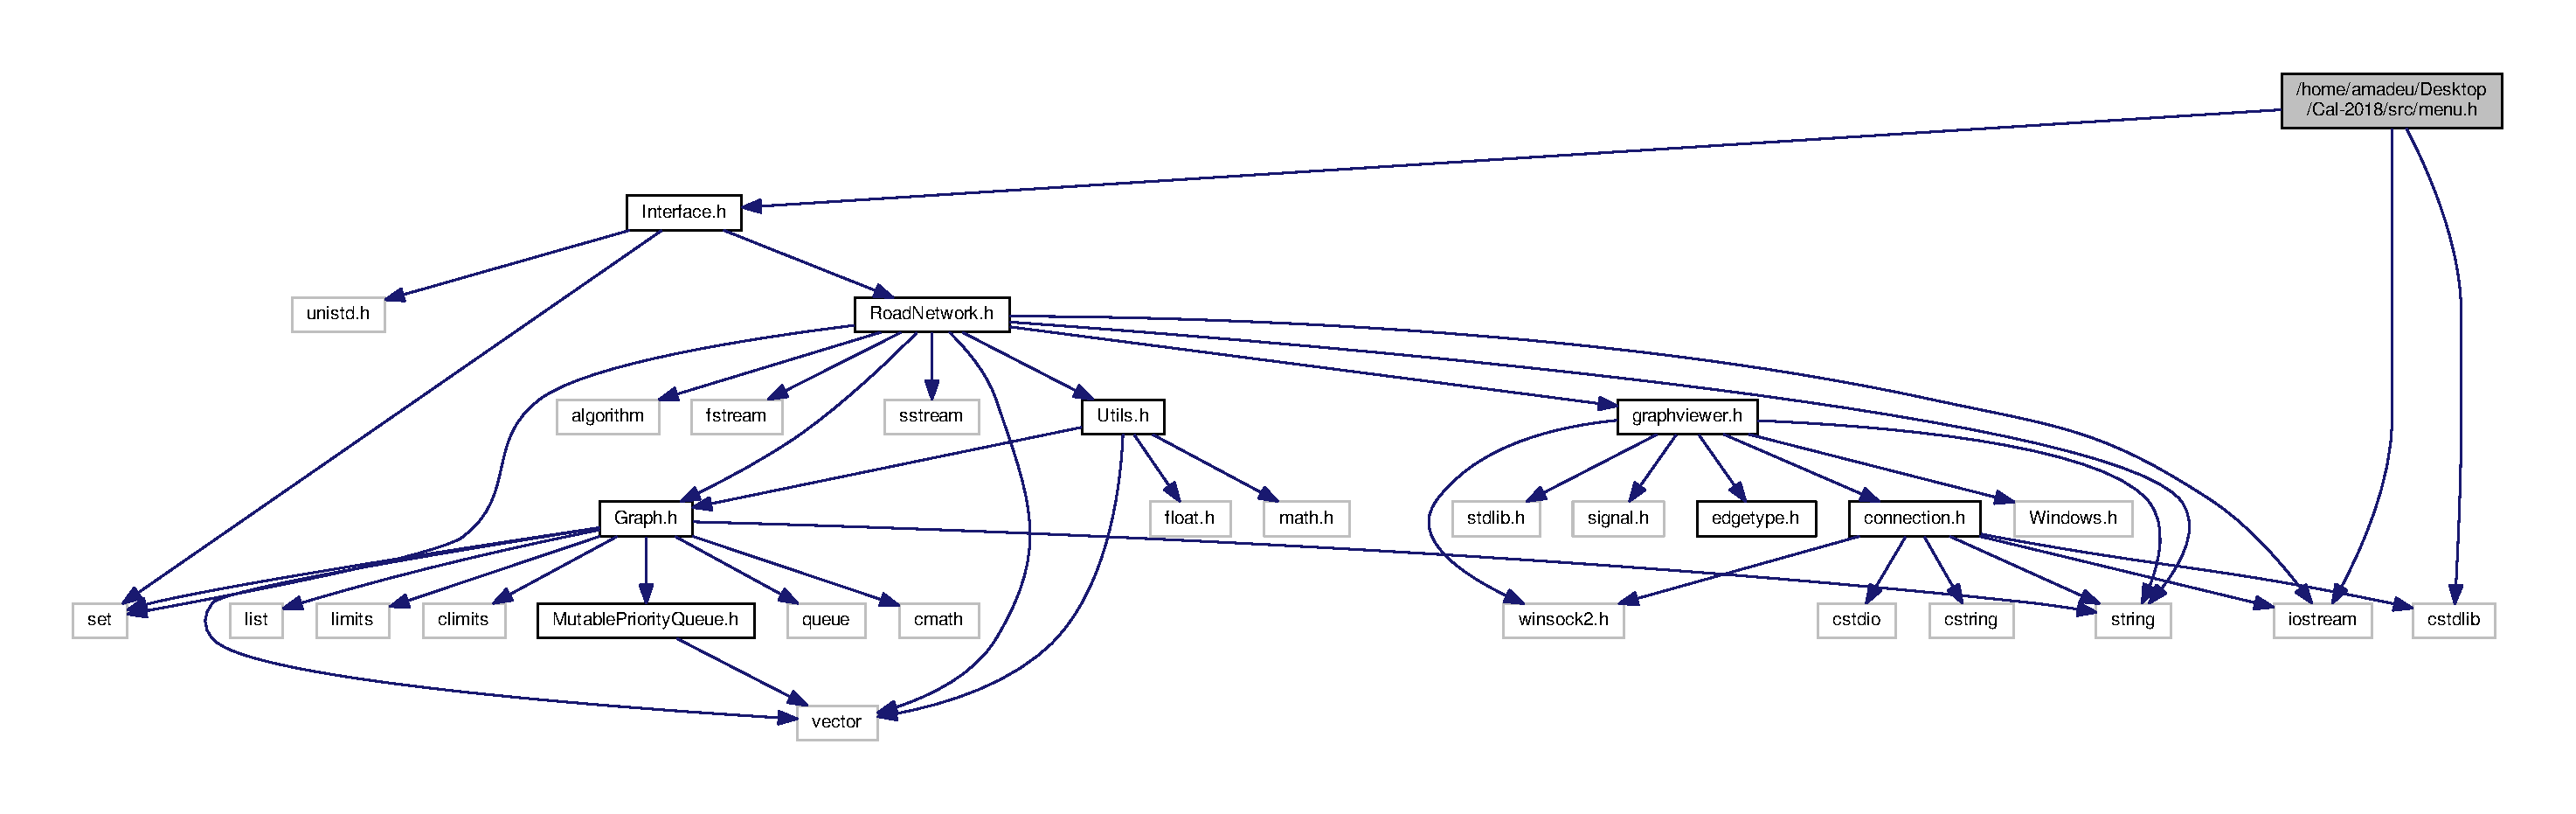
\includegraphics[width=350pt]{menu_8h__incl}
\end{center}
\end{figure}
This graph shows which files directly or indirectly include this file\+:\nopagebreak
\begin{figure}[H]
\begin{center}
\leavevmode
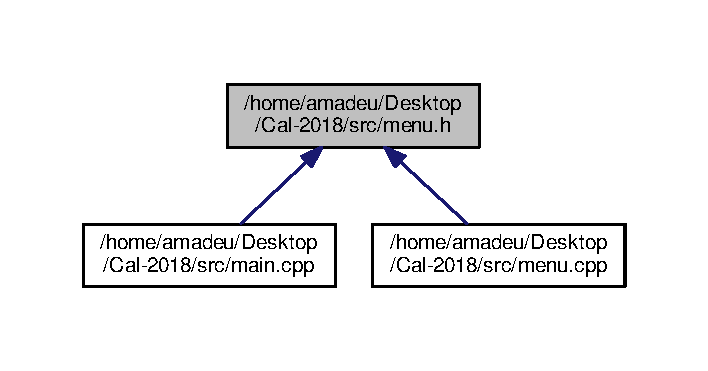
\includegraphics[width=340pt]{menu_8h__dep__incl}
\end{center}
\end{figure}
\subsection*{Functions}
\begin{DoxyCompactItemize}
\item 
void \hyperlink{menu_8h_a2a0e843767aeea4f433a28b9c54f573a}{menu} ()
\end{DoxyCompactItemize}


\subsection{Function Documentation}
\index{menu.\+h@{menu.\+h}!menu@{menu}}
\index{menu@{menu}!menu.\+h@{menu.\+h}}
\subsubsection[{\texorpdfstring{menu()}{menu()}}]{\setlength{\rightskip}{0pt plus 5cm}void menu (
\begin{DoxyParamCaption}
{}
\end{DoxyParamCaption}
)}\hypertarget{menu_8h_a2a0e843767aeea4f433a28b9c54f573a}{}\label{menu_8h_a2a0e843767aeea4f433a28b9c54f573a}
Menu do programa 
\hypertarget{MutablePriorityQueue_8h}{}\section{/home/amadeu/\+Desktop/\+Cal-\/2018/src/\+Mutable\+Priority\+Queue.h File Reference}
\label{MutablePriorityQueue_8h}\index{/home/amadeu/\+Desktop/\+Cal-\/2018/src/\+Mutable\+Priority\+Queue.\+h@{/home/amadeu/\+Desktop/\+Cal-\/2018/src/\+Mutable\+Priority\+Queue.\+h}}
{\ttfamily \#include $<$vector$>$}\\*
Include dependency graph for Mutable\+Priority\+Queue.\+h\+:\nopagebreak
\begin{figure}[H]
\begin{center}
\leavevmode
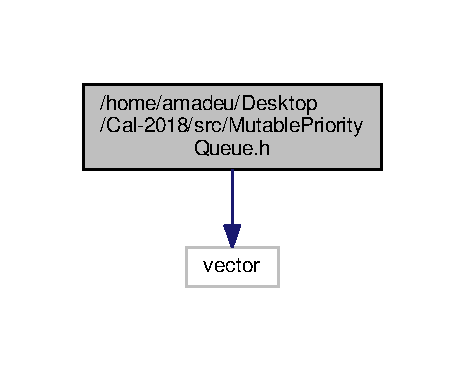
\includegraphics[width=223pt]{MutablePriorityQueue_8h__incl}
\end{center}
\end{figure}
This graph shows which files directly or indirectly include this file\+:\nopagebreak
\begin{figure}[H]
\begin{center}
\leavevmode
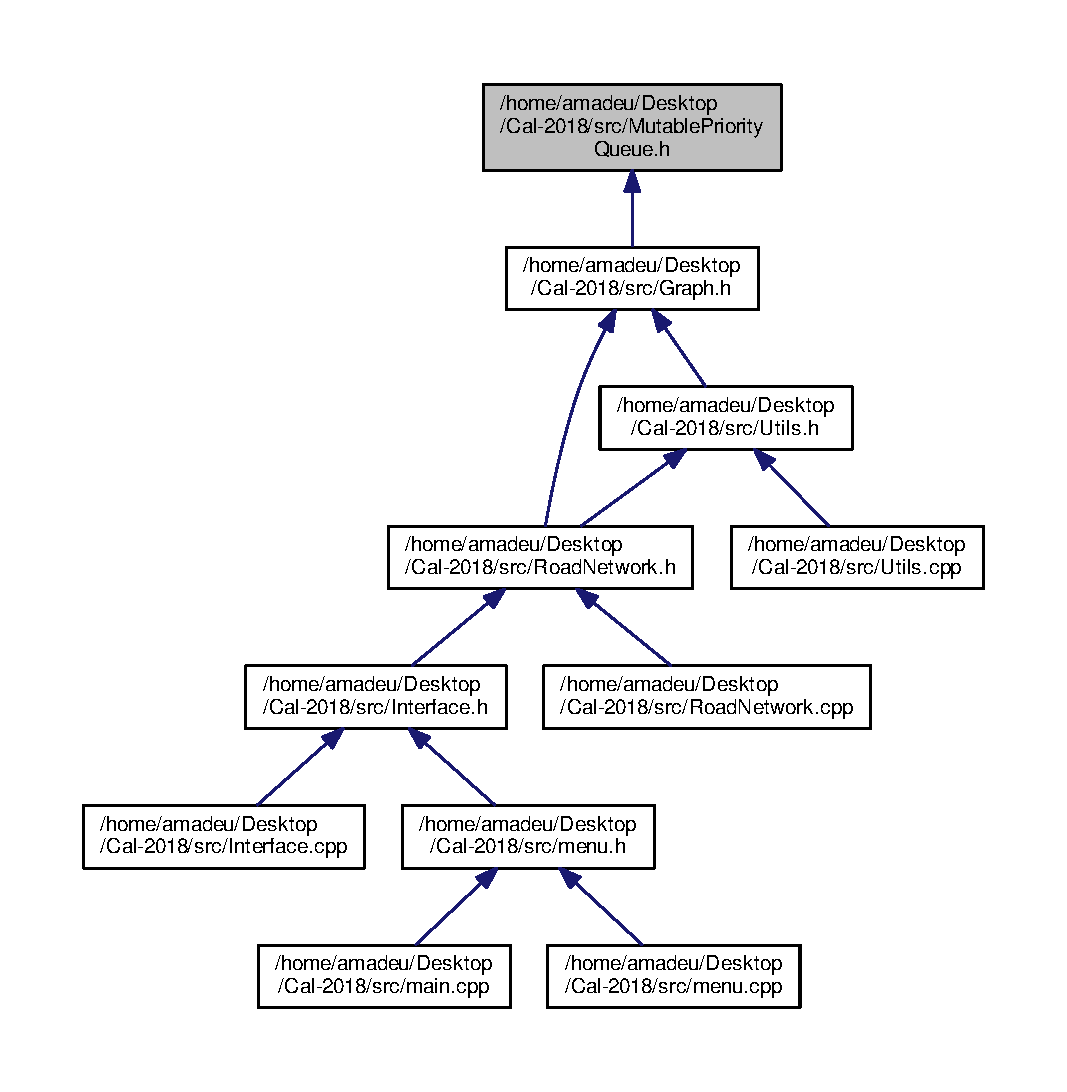
\includegraphics[width=350pt]{MutablePriorityQueue_8h__dep__incl}
\end{center}
\end{figure}
\subsection*{Classes}
\begin{DoxyCompactItemize}
\item 
class \hyperlink{classMutablePriorityQueue}{Mutable\+Priority\+Queue$<$ T $>$}
\end{DoxyCompactItemize}
\subsection*{Macros}
\begin{DoxyCompactItemize}
\item 
\#define \hyperlink{MutablePriorityQueue_8h_a915a9564b15f2c25e828da2e9a05769c}{parent}(\hyperlink{menu_8cpp_a98862a04b438a5359a542f245ca97b62}{i})~((\hyperlink{menu_8cpp_a98862a04b438a5359a542f245ca97b62}{i}) $>$$>$ 1)  /$\ast$ \hyperlink{menu_8cpp_a98862a04b438a5359a542f245ca97b62}{i} / 2 $\ast$/
\item 
\#define \hyperlink{MutablePriorityQueue_8h_ac84ef3998ba958fd8abf03d08cc5ffcb}{left\+Child}(\hyperlink{menu_8cpp_a98862a04b438a5359a542f245ca97b62}{i})~((\hyperlink{menu_8cpp_a98862a04b438a5359a542f245ca97b62}{i}) $<$$<$ 1)  /$\ast$ \hyperlink{menu_8cpp_a98862a04b438a5359a542f245ca97b62}{i} $\ast$ 2 $\ast$/
\end{DoxyCompactItemize}


\subsection{Macro Definition Documentation}
\index{Mutable\+Priority\+Queue.\+h@{Mutable\+Priority\+Queue.\+h}!left\+Child@{left\+Child}}
\index{left\+Child@{left\+Child}!Mutable\+Priority\+Queue.\+h@{Mutable\+Priority\+Queue.\+h}}
\subsubsection[{\texorpdfstring{left\+Child}{leftChild}}]{\setlength{\rightskip}{0pt plus 5cm}\#define left\+Child(
\begin{DoxyParamCaption}
\item[{}]{{\bf i}}
\end{DoxyParamCaption}
)~(({\bf i}) $<$$<$ 1)  /$\ast$ {\bf i} $\ast$ 2 $\ast$/}\hypertarget{MutablePriorityQueue_8h_ac84ef3998ba958fd8abf03d08cc5ffcb}{}\label{MutablePriorityQueue_8h_ac84ef3998ba958fd8abf03d08cc5ffcb}
\index{Mutable\+Priority\+Queue.\+h@{Mutable\+Priority\+Queue.\+h}!parent@{parent}}
\index{parent@{parent}!Mutable\+Priority\+Queue.\+h@{Mutable\+Priority\+Queue.\+h}}
\subsubsection[{\texorpdfstring{parent}{parent}}]{\setlength{\rightskip}{0pt plus 5cm}\#define parent(
\begin{DoxyParamCaption}
\item[{}]{{\bf i}}
\end{DoxyParamCaption}
)~(({\bf i}) $>$$>$ 1)  /$\ast$ {\bf i} / 2 $\ast$/}\hypertarget{MutablePriorityQueue_8h_a915a9564b15f2c25e828da2e9a05769c}{}\label{MutablePriorityQueue_8h_a915a9564b15f2c25e828da2e9a05769c}

\hypertarget{RoadNetwork_8cpp}{}\section{/home/amadeu/\+Desktop/\+Cal-\/2018/src/\+Road\+Network.cpp File Reference}
\label{RoadNetwork_8cpp}\index{/home/amadeu/\+Desktop/\+Cal-\/2018/src/\+Road\+Network.\+cpp@{/home/amadeu/\+Desktop/\+Cal-\/2018/src/\+Road\+Network.\+cpp}}
{\ttfamily \#include \char`\"{}Road\+Network.\+h\char`\"{}}\\*
Include dependency graph for Road\+Network.\+cpp\+:\nopagebreak
\begin{figure}[H]
\begin{center}
\leavevmode
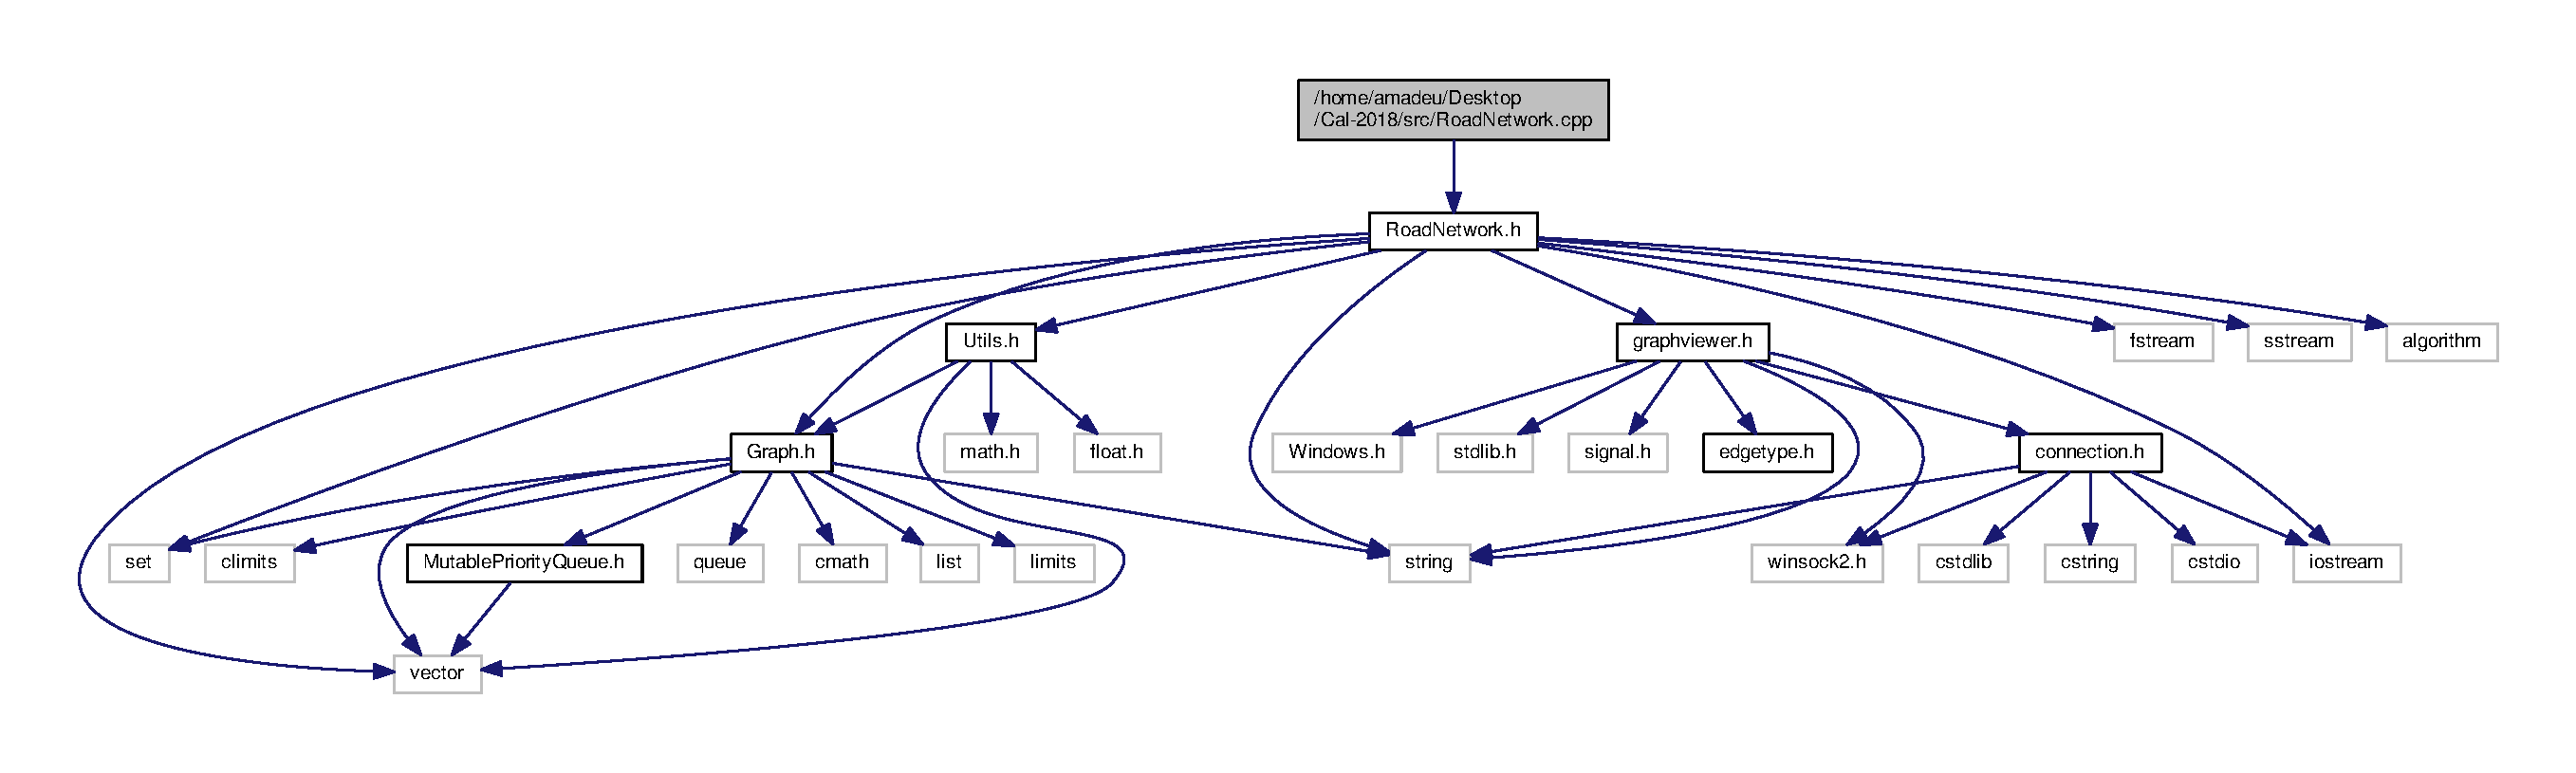
\includegraphics[width=350pt]{RoadNetwork_8cpp__incl}
\end{center}
\end{figure}
\subsection*{Functions}
\begin{DoxyCompactItemize}
\item 
bool \hyperlink{RoadNetwork_8cpp_a76a4ba4ef25d3eb62249d90a3d128bc5}{compare\+Vector\+Edges} (\hyperlink{classEdge}{Edge}$<$ int $>$ $\ast$edge1, \hyperlink{classEdge}{Edge}$<$ int $>$ $\ast$edge2)
\end{DoxyCompactItemize}


\subsection{Function Documentation}
\index{Road\+Network.\+cpp@{Road\+Network.\+cpp}!compare\+Vector\+Edges@{compare\+Vector\+Edges}}
\index{compare\+Vector\+Edges@{compare\+Vector\+Edges}!Road\+Network.\+cpp@{Road\+Network.\+cpp}}
\subsubsection[{\texorpdfstring{compare\+Vector\+Edges(\+Edge$<$ int $>$ $\ast$edge1, Edge$<$ int $>$ $\ast$edge2)}{compareVectorEdges(Edge< int > *edge1, Edge< int > *edge2)}}]{\setlength{\rightskip}{0pt plus 5cm}bool compare\+Vector\+Edges (
\begin{DoxyParamCaption}
\item[{{\bf Edge}$<$ int $>$ $\ast$}]{edge1, }
\item[{{\bf Edge}$<$ int $>$ $\ast$}]{edge2}
\end{DoxyParamCaption}
)}\hypertarget{RoadNetwork_8cpp_a76a4ba4ef25d3eb62249d90a3d128bc5}{}\label{RoadNetwork_8cpp_a76a4ba4ef25d3eb62249d90a3d128bc5}

\hypertarget{RoadNetwork_8h}{}\section{/home/amadeu/\+Desktop/\+Cal-\/2018/src/\+Road\+Network.h File Reference}
\label{RoadNetwork_8h}\index{/home/amadeu/\+Desktop/\+Cal-\/2018/src/\+Road\+Network.\+h@{/home/amadeu/\+Desktop/\+Cal-\/2018/src/\+Road\+Network.\+h}}
{\ttfamily \#include $<$iostream$>$}\\*
{\ttfamily \#include $<$fstream$>$}\\*
{\ttfamily \#include $<$sstream$>$}\\*
{\ttfamily \#include $<$string$>$}\\*
{\ttfamily \#include $<$algorithm$>$}\\*
{\ttfamily \#include $<$vector$>$}\\*
{\ttfamily \#include \char`\"{}Graph.\+h\char`\"{}}\\*
{\ttfamily \#include \char`\"{}graphviewer.\+h\char`\"{}}\\*
{\ttfamily \#include \char`\"{}Utils.\+h\char`\"{}}\\*
{\ttfamily \#include $<$set$>$}\\*
Include dependency graph for Road\+Network.\+h\+:\nopagebreak
\begin{figure}[H]
\begin{center}
\leavevmode
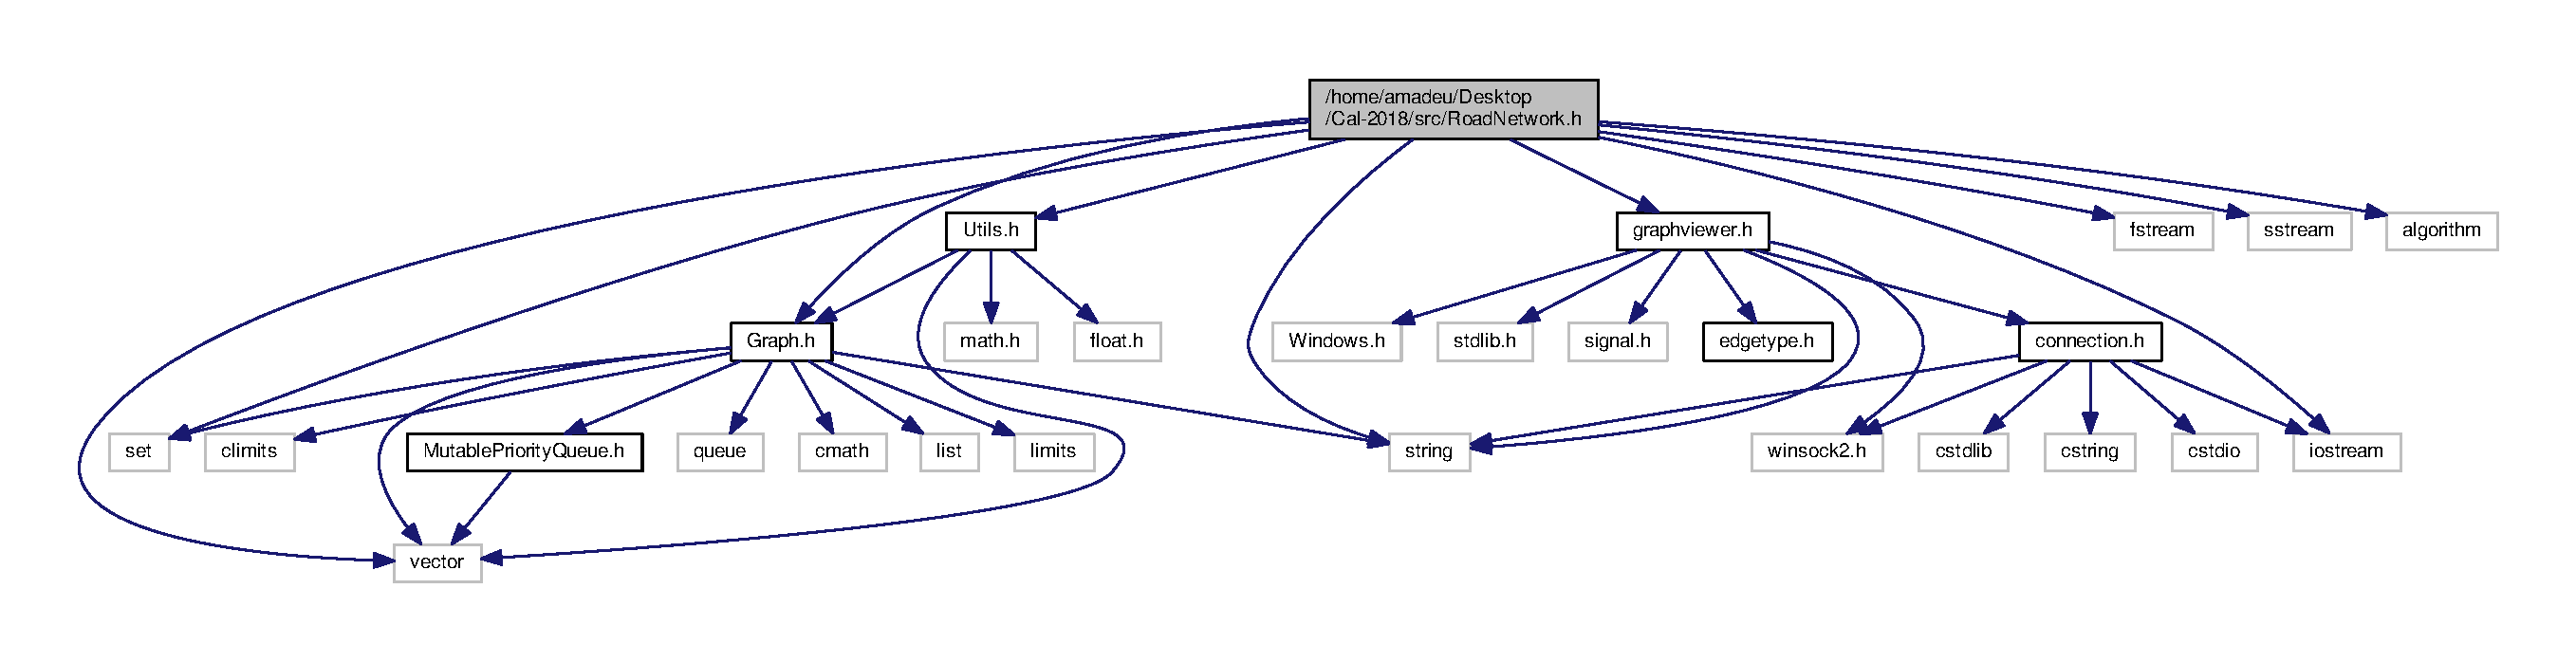
\includegraphics[width=350pt]{RoadNetwork_8h__incl}
\end{center}
\end{figure}
This graph shows which files directly or indirectly include this file\+:\nopagebreak
\begin{figure}[H]
\begin{center}
\leavevmode
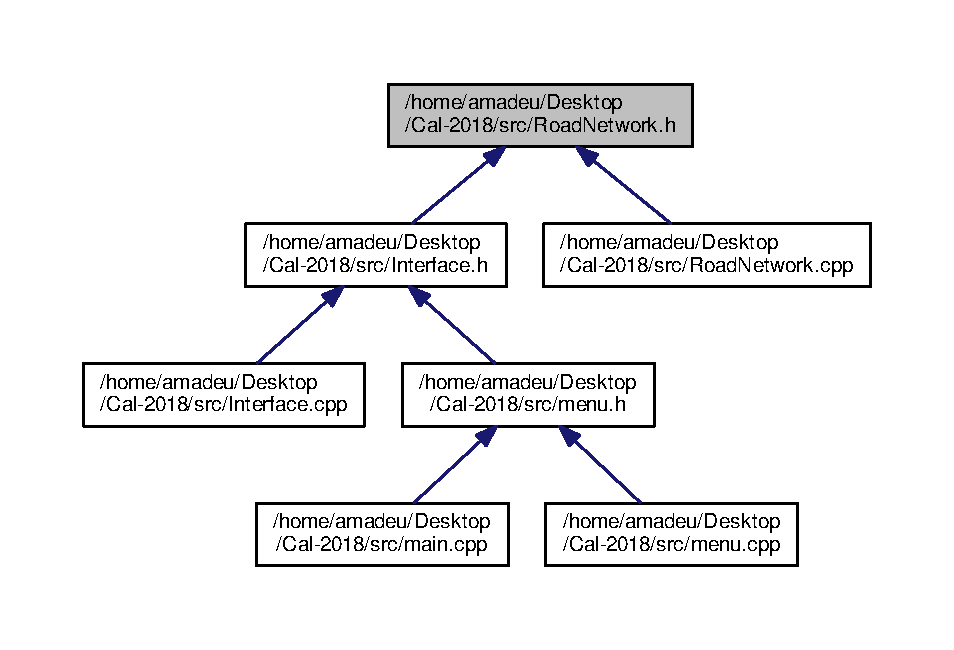
\includegraphics[width=350pt]{RoadNetwork_8h__dep__incl}
\end{center}
\end{figure}
\subsection*{Classes}
\begin{DoxyCompactItemize}
\item 
class \hyperlink{classRoadNetwork}{Road\+Network}
\end{DoxyCompactItemize}
\subsection*{Macros}
\begin{DoxyCompactItemize}
\item 
\#define \hyperlink{RoadNetwork_8h_a6e6e0f0a07b275692baea5c5ea99ae45}{D\+E\+F\+A\+U\+L\+T\+\_\+\+V\+E\+R\+T\+E\+X\+\_\+\+C\+O\+L\+OR}~\char`\"{}blue\char`\"{}
\item 
\#define \hyperlink{RoadNetwork_8h_afc7c125091ba180d90d5c7aa19645d38}{D\+E\+F\+A\+U\+L\+T\+\_\+\+E\+D\+G\+E\+\_\+\+C\+O\+L\+OR}~\char`\"{}green\char`\"{}
\item 
\#define \hyperlink{RoadNetwork_8h_a5d57b679ed7a8e206acb4b2e86534120}{H\+I\+G\+H\+L\+I\+G\+H\+T\+E\+D\+\_\+\+V\+E\+R\+T\+E\+X\+\_\+\+C\+O\+L\+OR}~\char`\"{}yellow\char`\"{}
\item 
\#define \hyperlink{RoadNetwork_8h_a973c5f767642717d927a10c4ba7b0536}{H\+I\+G\+H\+L\+I\+G\+H\+T\+E\+D\+\_\+\+E\+D\+G\+E\+\_\+\+C\+O\+L\+OR}~\char`\"{}yellow\char`\"{}
\item 
\#define \hyperlink{RoadNetwork_8h_aab9747c5846f722e12157db553d5fbaa}{M\+E\+D\+I\+U\+M\+\_\+\+T\+R\+A\+F\+F\+IC}~\char`\"{}orange\char`\"{}
\item 
\#define \hyperlink{RoadNetwork_8h_a88ca92279b5d6c46600c7bbec05cd421}{H\+I\+G\+H\+\_\+\+T\+R\+A\+F\+F\+IC}~\char`\"{}red\char`\"{}
\item 
\#define \hyperlink{RoadNetwork_8h_a85f4a39e351bd60a328dd9cf8cc4dae0}{B\+L\+O\+C\+K\+E\+D\+\_\+\+E\+D\+G\+E\+\_\+\+C\+O\+L\+OR}~\char`\"{}black\char`\"{}
\end{DoxyCompactItemize}


\subsection{Macro Definition Documentation}
\index{Road\+Network.\+h@{Road\+Network.\+h}!B\+L\+O\+C\+K\+E\+D\+\_\+\+E\+D\+G\+E\+\_\+\+C\+O\+L\+OR@{B\+L\+O\+C\+K\+E\+D\+\_\+\+E\+D\+G\+E\+\_\+\+C\+O\+L\+OR}}
\index{B\+L\+O\+C\+K\+E\+D\+\_\+\+E\+D\+G\+E\+\_\+\+C\+O\+L\+OR@{B\+L\+O\+C\+K\+E\+D\+\_\+\+E\+D\+G\+E\+\_\+\+C\+O\+L\+OR}!Road\+Network.\+h@{Road\+Network.\+h}}
\subsubsection[{\texorpdfstring{B\+L\+O\+C\+K\+E\+D\+\_\+\+E\+D\+G\+E\+\_\+\+C\+O\+L\+OR}{BLOCKED_EDGE_COLOR}}]{\setlength{\rightskip}{0pt plus 5cm}\#define B\+L\+O\+C\+K\+E\+D\+\_\+\+E\+D\+G\+E\+\_\+\+C\+O\+L\+OR~\char`\"{}black\char`\"{}}\hypertarget{RoadNetwork_8h_a85f4a39e351bd60a328dd9cf8cc4dae0}{}\label{RoadNetwork_8h_a85f4a39e351bd60a328dd9cf8cc4dae0}
Cor das edges bloqueadas \index{Road\+Network.\+h@{Road\+Network.\+h}!D\+E\+F\+A\+U\+L\+T\+\_\+\+E\+D\+G\+E\+\_\+\+C\+O\+L\+OR@{D\+E\+F\+A\+U\+L\+T\+\_\+\+E\+D\+G\+E\+\_\+\+C\+O\+L\+OR}}
\index{D\+E\+F\+A\+U\+L\+T\+\_\+\+E\+D\+G\+E\+\_\+\+C\+O\+L\+OR@{D\+E\+F\+A\+U\+L\+T\+\_\+\+E\+D\+G\+E\+\_\+\+C\+O\+L\+OR}!Road\+Network.\+h@{Road\+Network.\+h}}
\subsubsection[{\texorpdfstring{D\+E\+F\+A\+U\+L\+T\+\_\+\+E\+D\+G\+E\+\_\+\+C\+O\+L\+OR}{DEFAULT_EDGE_COLOR}}]{\setlength{\rightskip}{0pt plus 5cm}\#define D\+E\+F\+A\+U\+L\+T\+\_\+\+E\+D\+G\+E\+\_\+\+C\+O\+L\+OR~\char`\"{}green\char`\"{}}\hypertarget{RoadNetwork_8h_afc7c125091ba180d90d5c7aa19645d38}{}\label{RoadNetwork_8h_afc7c125091ba180d90d5c7aa19645d38}
Cor das edges com pouco transito \index{Road\+Network.\+h@{Road\+Network.\+h}!D\+E\+F\+A\+U\+L\+T\+\_\+\+V\+E\+R\+T\+E\+X\+\_\+\+C\+O\+L\+OR@{D\+E\+F\+A\+U\+L\+T\+\_\+\+V\+E\+R\+T\+E\+X\+\_\+\+C\+O\+L\+OR}}
\index{D\+E\+F\+A\+U\+L\+T\+\_\+\+V\+E\+R\+T\+E\+X\+\_\+\+C\+O\+L\+OR@{D\+E\+F\+A\+U\+L\+T\+\_\+\+V\+E\+R\+T\+E\+X\+\_\+\+C\+O\+L\+OR}!Road\+Network.\+h@{Road\+Network.\+h}}
\subsubsection[{\texorpdfstring{D\+E\+F\+A\+U\+L\+T\+\_\+\+V\+E\+R\+T\+E\+X\+\_\+\+C\+O\+L\+OR}{DEFAULT_VERTEX_COLOR}}]{\setlength{\rightskip}{0pt plus 5cm}\#define D\+E\+F\+A\+U\+L\+T\+\_\+\+V\+E\+R\+T\+E\+X\+\_\+\+C\+O\+L\+OR~\char`\"{}blue\char`\"{}}\hypertarget{RoadNetwork_8h_a6e6e0f0a07b275692baea5c5ea99ae45}{}\label{RoadNetwork_8h_a6e6e0f0a07b275692baea5c5ea99ae45}
Cor padrao dos vertices \index{Road\+Network.\+h@{Road\+Network.\+h}!H\+I\+G\+H\+\_\+\+T\+R\+A\+F\+F\+IC@{H\+I\+G\+H\+\_\+\+T\+R\+A\+F\+F\+IC}}
\index{H\+I\+G\+H\+\_\+\+T\+R\+A\+F\+F\+IC@{H\+I\+G\+H\+\_\+\+T\+R\+A\+F\+F\+IC}!Road\+Network.\+h@{Road\+Network.\+h}}
\subsubsection[{\texorpdfstring{H\+I\+G\+H\+\_\+\+T\+R\+A\+F\+F\+IC}{HIGH_TRAFFIC}}]{\setlength{\rightskip}{0pt plus 5cm}\#define H\+I\+G\+H\+\_\+\+T\+R\+A\+F\+F\+IC~\char`\"{}red\char`\"{}}\hypertarget{RoadNetwork_8h_a88ca92279b5d6c46600c7bbec05cd421}{}\label{RoadNetwork_8h_a88ca92279b5d6c46600c7bbec05cd421}
Cor das edges com muito transito \index{Road\+Network.\+h@{Road\+Network.\+h}!H\+I\+G\+H\+L\+I\+G\+H\+T\+E\+D\+\_\+\+E\+D\+G\+E\+\_\+\+C\+O\+L\+OR@{H\+I\+G\+H\+L\+I\+G\+H\+T\+E\+D\+\_\+\+E\+D\+G\+E\+\_\+\+C\+O\+L\+OR}}
\index{H\+I\+G\+H\+L\+I\+G\+H\+T\+E\+D\+\_\+\+E\+D\+G\+E\+\_\+\+C\+O\+L\+OR@{H\+I\+G\+H\+L\+I\+G\+H\+T\+E\+D\+\_\+\+E\+D\+G\+E\+\_\+\+C\+O\+L\+OR}!Road\+Network.\+h@{Road\+Network.\+h}}
\subsubsection[{\texorpdfstring{H\+I\+G\+H\+L\+I\+G\+H\+T\+E\+D\+\_\+\+E\+D\+G\+E\+\_\+\+C\+O\+L\+OR}{HIGHLIGHTED_EDGE_COLOR}}]{\setlength{\rightskip}{0pt plus 5cm}\#define H\+I\+G\+H\+L\+I\+G\+H\+T\+E\+D\+\_\+\+E\+D\+G\+E\+\_\+\+C\+O\+L\+OR~\char`\"{}yellow\char`\"{}}\hypertarget{RoadNetwork_8h_a973c5f767642717d927a10c4ba7b0536}{}\label{RoadNetwork_8h_a973c5f767642717d927a10c4ba7b0536}
Cor das edges que estao a ser representadas como percurso \index{Road\+Network.\+h@{Road\+Network.\+h}!H\+I\+G\+H\+L\+I\+G\+H\+T\+E\+D\+\_\+\+V\+E\+R\+T\+E\+X\+\_\+\+C\+O\+L\+OR@{H\+I\+G\+H\+L\+I\+G\+H\+T\+E\+D\+\_\+\+V\+E\+R\+T\+E\+X\+\_\+\+C\+O\+L\+OR}}
\index{H\+I\+G\+H\+L\+I\+G\+H\+T\+E\+D\+\_\+\+V\+E\+R\+T\+E\+X\+\_\+\+C\+O\+L\+OR@{H\+I\+G\+H\+L\+I\+G\+H\+T\+E\+D\+\_\+\+V\+E\+R\+T\+E\+X\+\_\+\+C\+O\+L\+OR}!Road\+Network.\+h@{Road\+Network.\+h}}
\subsubsection[{\texorpdfstring{H\+I\+G\+H\+L\+I\+G\+H\+T\+E\+D\+\_\+\+V\+E\+R\+T\+E\+X\+\_\+\+C\+O\+L\+OR}{HIGHLIGHTED_VERTEX_COLOR}}]{\setlength{\rightskip}{0pt plus 5cm}\#define H\+I\+G\+H\+L\+I\+G\+H\+T\+E\+D\+\_\+\+V\+E\+R\+T\+E\+X\+\_\+\+C\+O\+L\+OR~\char`\"{}yellow\char`\"{}}\hypertarget{RoadNetwork_8h_a5d57b679ed7a8e206acb4b2e86534120}{}\label{RoadNetwork_8h_a5d57b679ed7a8e206acb4b2e86534120}
Cor dos vertices que estao a ser representados como percurso \index{Road\+Network.\+h@{Road\+Network.\+h}!M\+E\+D\+I\+U\+M\+\_\+\+T\+R\+A\+F\+F\+IC@{M\+E\+D\+I\+U\+M\+\_\+\+T\+R\+A\+F\+F\+IC}}
\index{M\+E\+D\+I\+U\+M\+\_\+\+T\+R\+A\+F\+F\+IC@{M\+E\+D\+I\+U\+M\+\_\+\+T\+R\+A\+F\+F\+IC}!Road\+Network.\+h@{Road\+Network.\+h}}
\subsubsection[{\texorpdfstring{M\+E\+D\+I\+U\+M\+\_\+\+T\+R\+A\+F\+F\+IC}{MEDIUM_TRAFFIC}}]{\setlength{\rightskip}{0pt plus 5cm}\#define M\+E\+D\+I\+U\+M\+\_\+\+T\+R\+A\+F\+F\+IC~\char`\"{}orange\char`\"{}}\hypertarget{RoadNetwork_8h_aab9747c5846f722e12157db553d5fbaa}{}\label{RoadNetwork_8h_aab9747c5846f722e12157db553d5fbaa}
Cor das edges com algum transito 
\hypertarget{Utils_8cpp}{}\section{/home/amadeu/\+Desktop/\+Cal-\/2018/src/\+Utils.cpp File Reference}
\label{Utils_8cpp}\index{/home/amadeu/\+Desktop/\+Cal-\/2018/src/\+Utils.\+cpp@{/home/amadeu/\+Desktop/\+Cal-\/2018/src/\+Utils.\+cpp}}
{\ttfamily \#include $<$iostream$>$}\\*
{\ttfamily \#include \char`\"{}Utils.\+h\char`\"{}}\\*
Include dependency graph for Utils.\+cpp\+:\nopagebreak
\begin{figure}[H]
\begin{center}
\leavevmode
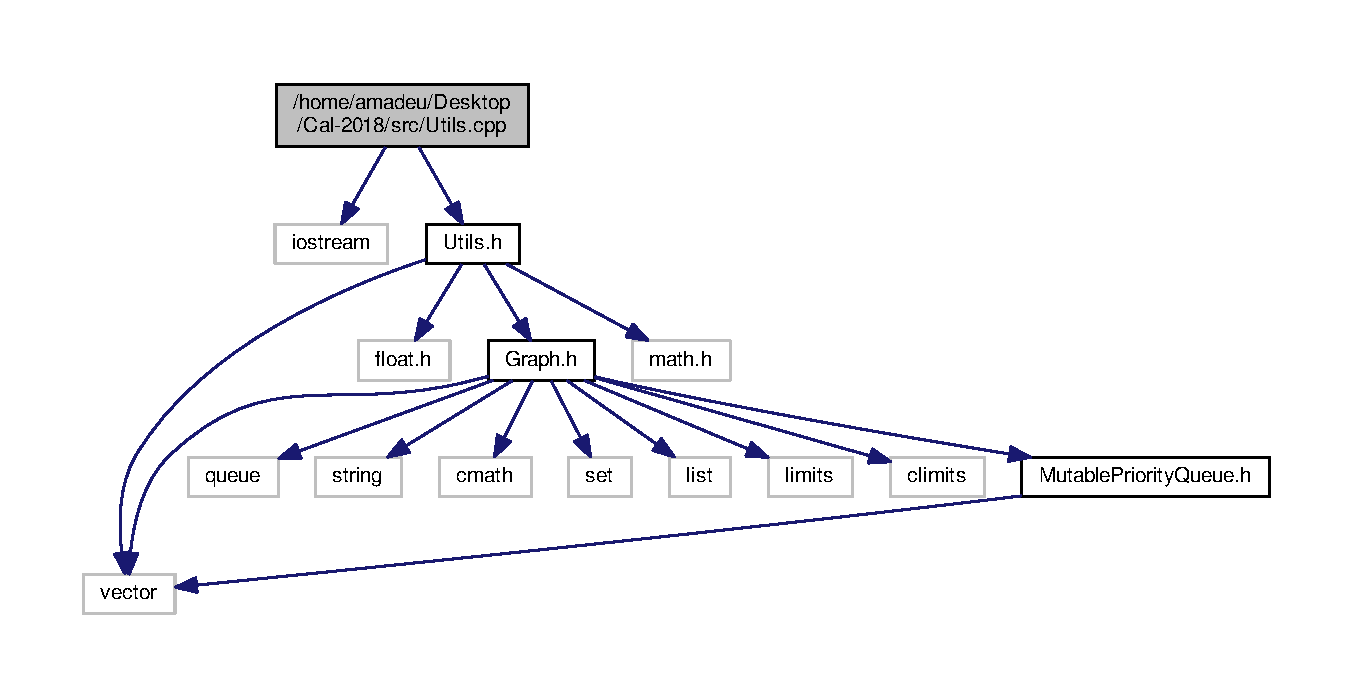
\includegraphics[width=350pt]{Utils_8cpp__incl}
\end{center}
\end{figure}
\subsection*{Functions}
\begin{DoxyCompactItemize}
\item 
int \hyperlink{Utils_8cpp_a98eb7eefa7ea484f580e08dd3dbddc9f}{resize\+Lat} (long double lat)
\item 
int \hyperlink{Utils_8cpp_acad80794f9e879a5f1be4aa45ba317de}{resize\+Lon} (long double lon)
\end{DoxyCompactItemize}


\subsection{Function Documentation}
\index{Utils.\+cpp@{Utils.\+cpp}!resize\+Lat@{resize\+Lat}}
\index{resize\+Lat@{resize\+Lat}!Utils.\+cpp@{Utils.\+cpp}}
\subsubsection[{\texorpdfstring{resize\+Lat(long double lat)}{resizeLat(long double lat)}}]{\setlength{\rightskip}{0pt plus 5cm}int resize\+Lat (
\begin{DoxyParamCaption}
\item[{long double}]{lat}
\end{DoxyParamCaption}
)}\hypertarget{Utils_8cpp_a98eb7eefa7ea484f580e08dd3dbddc9f}{}\label{Utils_8cpp_a98eb7eefa7ea484f580e08dd3dbddc9f}
Calcula a posicao relativa, no mapa, da latitude dada, tendo por base o tamanho do mapa e as suas coordenadas extremas 
\begin{DoxyParams}{Parameters}
{\em lat} & latitude \\
\hline
\end{DoxyParams}
\begin{DoxyReturn}{Returns}
nova posicao 
\end{DoxyReturn}
\index{Utils.\+cpp@{Utils.\+cpp}!resize\+Lon@{resize\+Lon}}
\index{resize\+Lon@{resize\+Lon}!Utils.\+cpp@{Utils.\+cpp}}
\subsubsection[{\texorpdfstring{resize\+Lon(long double lon)}{resizeLon(long double lon)}}]{\setlength{\rightskip}{0pt plus 5cm}int resize\+Lon (
\begin{DoxyParamCaption}
\item[{long double}]{lon}
\end{DoxyParamCaption}
)}\hypertarget{Utils_8cpp_acad80794f9e879a5f1be4aa45ba317de}{}\label{Utils_8cpp_acad80794f9e879a5f1be4aa45ba317de}
Calcula a posicao relativa, no mapa, da longitude dada, tendo por base o tamanho do mapa e as suas coordenadas extremas 
\begin{DoxyParams}{Parameters}
{\em lon} & longitude \\
\hline
\end{DoxyParams}
\begin{DoxyReturn}{Returns}
nova posicao 
\end{DoxyReturn}

\hypertarget{Utils_8h}{}\section{/home/amadeu/\+Desktop/\+Cal-\/2018/src/\+Utils.h File Reference}
\label{Utils_8h}\index{/home/amadeu/\+Desktop/\+Cal-\/2018/src/\+Utils.\+h@{/home/amadeu/\+Desktop/\+Cal-\/2018/src/\+Utils.\+h}}
{\ttfamily \#include $<$vector$>$}\\*
{\ttfamily \#include $<$float.\+h$>$}\\*
{\ttfamily \#include \char`\"{}Graph.\+h\char`\"{}}\\*
{\ttfamily \#include \char`\"{}math.\+h\char`\"{}}\\*
Include dependency graph for Utils.\+h\+:\nopagebreak
\begin{figure}[H]
\begin{center}
\leavevmode
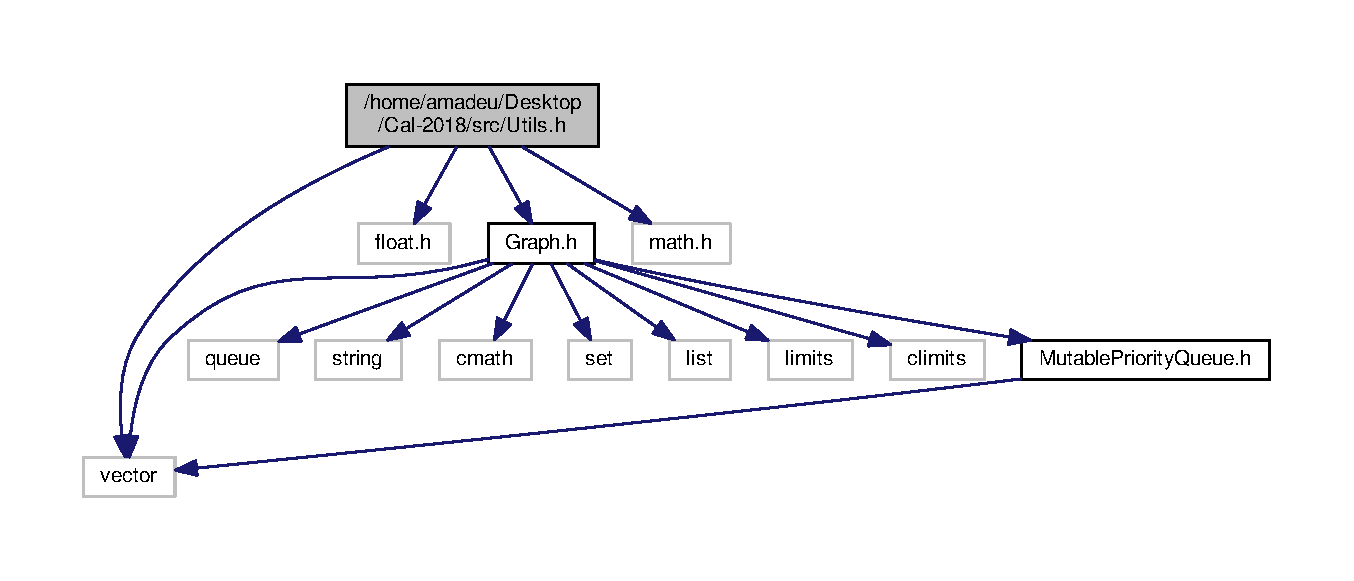
\includegraphics[width=350pt]{Utils_8h__incl}
\end{center}
\end{figure}
This graph shows which files directly or indirectly include this file\+:\nopagebreak
\begin{figure}[H]
\begin{center}
\leavevmode
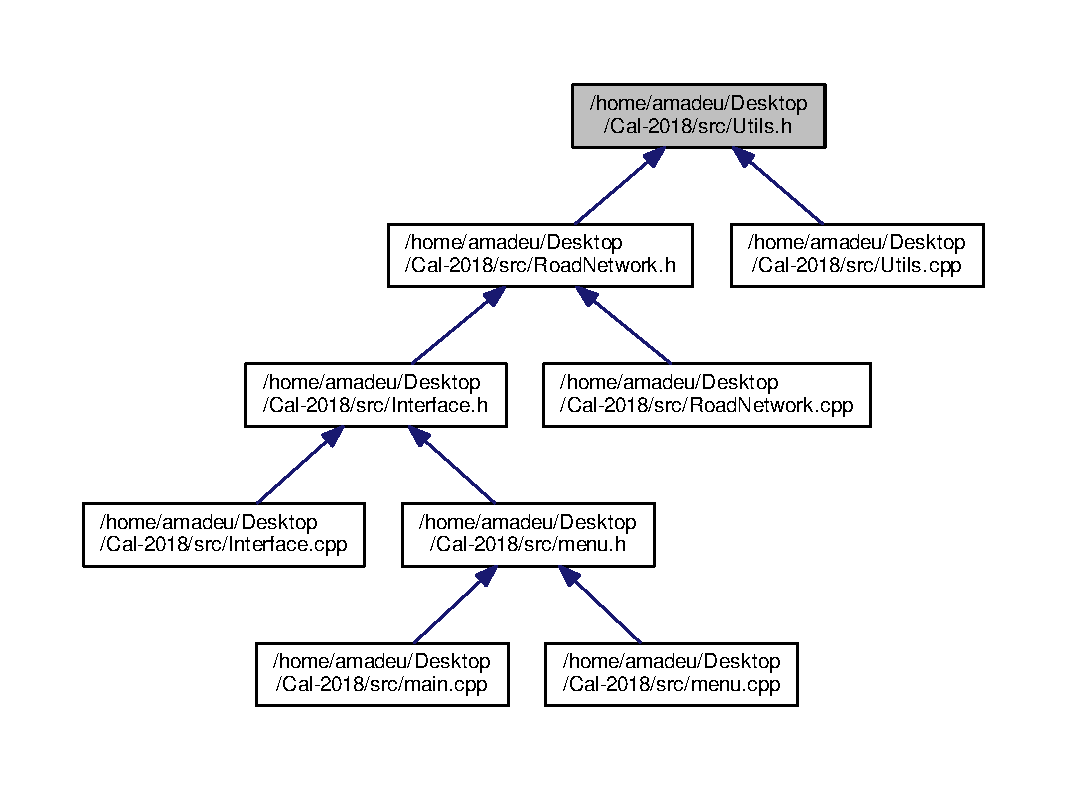
\includegraphics[width=350pt]{Utils_8h__dep__incl}
\end{center}
\end{figure}
\subsection*{Classes}
\begin{DoxyCompactItemize}
\item 
class \hyperlink{classLink}{Link}
\end{DoxyCompactItemize}
\subsection*{Macros}
\begin{DoxyCompactItemize}
\item 
\#define \hyperlink{Utils_8h_adbf4f46a396f0eda435971735dfc40cf}{G\+V\+\_\+\+W\+I\+D\+TH}~1157
\item 
\#define \hyperlink{Utils_8h_a39af482c8c6e43be2248b3ab2647ba48}{G\+V\+\_\+\+H\+E\+I\+G\+HT}~2405
\item 
\#define \hyperlink{Utils_8h_a4ca049c4214c92678b8916d12e048f77}{M\+I\+N\+\_\+\+L\+ON}~-\/9.\+5691
\item 
\#define \hyperlink{Utils_8h_a358c78b75d5814dfa0a6f64113344e3f}{M\+A\+X\+\_\+\+L\+ON}~-\/6.\+3940
\item 
\#define \hyperlink{Utils_8h_afb7fd15722eccf2cd90338aac9f88318}{M\+I\+N\+\_\+\+L\+AT}~36.\+8554
\item 
\#define \hyperlink{Utils_8h_a7ce12d8a28541150544bc0dfeb789e13}{M\+A\+X\+\_\+\+L\+AT}~41.\+9411
\end{DoxyCompactItemize}
\subsection*{Functions}
\begin{DoxyCompactItemize}
\item 
int \hyperlink{Utils_8h_a98eb7eefa7ea484f580e08dd3dbddc9f}{resize\+Lat} (long double lat)
\item 
int \hyperlink{Utils_8h_acad80794f9e879a5f1be4aa45ba317de}{resize\+Lon} (long double lon)
\end{DoxyCompactItemize}


\subsection{Macro Definition Documentation}
\index{Utils.\+h@{Utils.\+h}!G\+V\+\_\+\+H\+E\+I\+G\+HT@{G\+V\+\_\+\+H\+E\+I\+G\+HT}}
\index{G\+V\+\_\+\+H\+E\+I\+G\+HT@{G\+V\+\_\+\+H\+E\+I\+G\+HT}!Utils.\+h@{Utils.\+h}}
\subsubsection[{\texorpdfstring{G\+V\+\_\+\+H\+E\+I\+G\+HT}{GV_HEIGHT}}]{\setlength{\rightskip}{0pt plus 5cm}\#define G\+V\+\_\+\+H\+E\+I\+G\+HT~2405}\hypertarget{Utils_8h_a39af482c8c6e43be2248b3ab2647ba48}{}\label{Utils_8h_a39af482c8c6e43be2248b3ab2647ba48}
\index{Utils.\+h@{Utils.\+h}!G\+V\+\_\+\+W\+I\+D\+TH@{G\+V\+\_\+\+W\+I\+D\+TH}}
\index{G\+V\+\_\+\+W\+I\+D\+TH@{G\+V\+\_\+\+W\+I\+D\+TH}!Utils.\+h@{Utils.\+h}}
\subsubsection[{\texorpdfstring{G\+V\+\_\+\+W\+I\+D\+TH}{GV_WIDTH}}]{\setlength{\rightskip}{0pt plus 5cm}\#define G\+V\+\_\+\+W\+I\+D\+TH~1157}\hypertarget{Utils_8h_adbf4f46a396f0eda435971735dfc40cf}{}\label{Utils_8h_adbf4f46a396f0eda435971735dfc40cf}
\index{Utils.\+h@{Utils.\+h}!M\+A\+X\+\_\+\+L\+AT@{M\+A\+X\+\_\+\+L\+AT}}
\index{M\+A\+X\+\_\+\+L\+AT@{M\+A\+X\+\_\+\+L\+AT}!Utils.\+h@{Utils.\+h}}
\subsubsection[{\texorpdfstring{M\+A\+X\+\_\+\+L\+AT}{MAX_LAT}}]{\setlength{\rightskip}{0pt plus 5cm}\#define M\+A\+X\+\_\+\+L\+AT~41.\+9411}\hypertarget{Utils_8h_a7ce12d8a28541150544bc0dfeb789e13}{}\label{Utils_8h_a7ce12d8a28541150544bc0dfeb789e13}
\index{Utils.\+h@{Utils.\+h}!M\+A\+X\+\_\+\+L\+ON@{M\+A\+X\+\_\+\+L\+ON}}
\index{M\+A\+X\+\_\+\+L\+ON@{M\+A\+X\+\_\+\+L\+ON}!Utils.\+h@{Utils.\+h}}
\subsubsection[{\texorpdfstring{M\+A\+X\+\_\+\+L\+ON}{MAX_LON}}]{\setlength{\rightskip}{0pt plus 5cm}\#define M\+A\+X\+\_\+\+L\+ON~-\/6.\+3940}\hypertarget{Utils_8h_a358c78b75d5814dfa0a6f64113344e3f}{}\label{Utils_8h_a358c78b75d5814dfa0a6f64113344e3f}
\index{Utils.\+h@{Utils.\+h}!M\+I\+N\+\_\+\+L\+AT@{M\+I\+N\+\_\+\+L\+AT}}
\index{M\+I\+N\+\_\+\+L\+AT@{M\+I\+N\+\_\+\+L\+AT}!Utils.\+h@{Utils.\+h}}
\subsubsection[{\texorpdfstring{M\+I\+N\+\_\+\+L\+AT}{MIN_LAT}}]{\setlength{\rightskip}{0pt plus 5cm}\#define M\+I\+N\+\_\+\+L\+AT~36.\+8554}\hypertarget{Utils_8h_afb7fd15722eccf2cd90338aac9f88318}{}\label{Utils_8h_afb7fd15722eccf2cd90338aac9f88318}
\index{Utils.\+h@{Utils.\+h}!M\+I\+N\+\_\+\+L\+ON@{M\+I\+N\+\_\+\+L\+ON}}
\index{M\+I\+N\+\_\+\+L\+ON@{M\+I\+N\+\_\+\+L\+ON}!Utils.\+h@{Utils.\+h}}
\subsubsection[{\texorpdfstring{M\+I\+N\+\_\+\+L\+ON}{MIN_LON}}]{\setlength{\rightskip}{0pt plus 5cm}\#define M\+I\+N\+\_\+\+L\+ON~-\/9.\+5691}\hypertarget{Utils_8h_a4ca049c4214c92678b8916d12e048f77}{}\label{Utils_8h_a4ca049c4214c92678b8916d12e048f77}


\subsection{Function Documentation}
\index{Utils.\+h@{Utils.\+h}!resize\+Lat@{resize\+Lat}}
\index{resize\+Lat@{resize\+Lat}!Utils.\+h@{Utils.\+h}}
\subsubsection[{\texorpdfstring{resize\+Lat(long double lat)}{resizeLat(long double lat)}}]{\setlength{\rightskip}{0pt plus 5cm}int resize\+Lat (
\begin{DoxyParamCaption}
\item[{long double}]{lat}
\end{DoxyParamCaption}
)}\hypertarget{Utils_8h_a98eb7eefa7ea484f580e08dd3dbddc9f}{}\label{Utils_8h_a98eb7eefa7ea484f580e08dd3dbddc9f}
Calcula a posicao relativa, no mapa, da latitude dada, tendo por base o tamanho do mapa e as suas coordenadas extremas 
\begin{DoxyParams}{Parameters}
{\em lat} & latitude \\
\hline
\end{DoxyParams}
\begin{DoxyReturn}{Returns}
nova posicao 
\end{DoxyReturn}
\index{Utils.\+h@{Utils.\+h}!resize\+Lon@{resize\+Lon}}
\index{resize\+Lon@{resize\+Lon}!Utils.\+h@{Utils.\+h}}
\subsubsection[{\texorpdfstring{resize\+Lon(long double lon)}{resizeLon(long double lon)}}]{\setlength{\rightskip}{0pt plus 5cm}int resize\+Lon (
\begin{DoxyParamCaption}
\item[{long double}]{lon}
\end{DoxyParamCaption}
)}\hypertarget{Utils_8h_acad80794f9e879a5f1be4aa45ba317de}{}\label{Utils_8h_acad80794f9e879a5f1be4aa45ba317de}
Calcula a posicao relativa, no mapa, da longitude dada, tendo por base o tamanho do mapa e as suas coordenadas extremas 
\begin{DoxyParams}{Parameters}
{\em lon} & longitude \\
\hline
\end{DoxyParams}
\begin{DoxyReturn}{Returns}
nova posicao 
\end{DoxyReturn}

%--- End generated contents ---

% Index
\backmatter
\newpage
\phantomsection
\clearemptydoublepage
\addcontentsline{toc}{chapter}{Index}
\printindex

\end{document}
